\documentclass[a4paper]{article}
\usepackage{import}
\usepackage[utf8]{inputenc}
\usepackage[T1]{fontenc}
\usepackage{textcomp}
\usepackage[italian]{babel}
\usepackage{amsmath, amssymb}
\usepackage{booktabs,xltabular}
\usepackage{amsfonts}
\usepackage{subcaption}
\usepackage{amsthm}
\usepackage{cancel}
\usepackage{mdframed}
\usepackage{makecell}
\usepackage{float}
\usepackage{xcolor}
\usepackage{listings}
\usepackage{gensymb}
\usepackage{graphicx}
\usepackage{bodeplot}
\usepackage{physics}
\usepackage{tikz}
\usetikzlibrary{shapes, arrows, automata, petri, decorations.markings, decorations.pathreplacing, positioning, calc, quotes}
\usepackage{circuitikz}
\usepackage[label=corner]{karnaugh-map}
\graphicspath{{./figures/}}

% Set default font to sans-serif
\renewcommand{\familydefault}{\sfdefault} 
\usepackage{eulervm}

\usepackage{forest}

\usepackage{mathtools}
\DeclarePairedDelimiter\ceil{\lceil}{\rceil}
\DeclarePairedDelimiter\floor{\lfloor}{\rfloor}

% \usepackage{ntheorem}

\usepackage{import}
\usepackage{pdfpages}
\usepackage{transparent}
\usepackage{xcolor}

\usepackage{hyperref}
\hypersetup{
    colorlinks=false,
}

% Code blocks
\definecolor{codegreen}{rgb}{0,0.6,0}
\definecolor{codegray}{rgb}{0.5,0.5,0.5}
\definecolor{codepurple}{rgb}{0.58,0,0.82}
\definecolor{backcolour}{rgb}{0.95,0.95,0.95}

\lstdefinestyle{mystyle}{
	backgroundcolor=\color{backcolour},
	commentstyle=\color{codegreen},
	keywordstyle=\color{magenta},
	numberstyle=\tiny\color{codegray},
	stringstyle=\color{codepurple},
	basicstyle=\ttfamily\footnotesize,
	breakatwhitespace=false,
	breaklines=true,
	captionpos=b,
	keepspaces=true,
	numbers=left,
	numbersep=5pt,
	showspaces=false,
	showstringspaces=false,
	showtabs=false,
	tabsize=2
}

\lstset{style=mystyle}

\usepackage{color}
\usepackage{import}
\usepackage{pdfpages}
\usepackage{transparent}
\usepackage{xcolor}

% Example frame
\theoremstyle{definition}
\newmdtheoremenv[%
	linecolor=gray,leftmargin=0,%
	rightmargin=0,
	innertopmargin=8pt,%
	innerbottommargin=8pt,
	ntheorem]{example}{Esempio}[section]

% Important definition frame
\theoremstyle{definition}
\newmdtheoremenv[%
	linecolor=gray,leftmargin=0,%
	rightmargin=0,
	backgroundcolor=gray!40,%
	innertopmargin=8pt,%
	innerbottommargin=8pt,
	ntheorem]{definition}{Definizione}[section]

% Exercise frame
\theoremstyle{definition}
\newmdtheoremenv[%
	linecolor=gray,leftmargin=0,%
	rightmargin=0,
	innertopmargin=8pt,%
	innerbottommargin=8pt,
	ntheorem]{exercise}{Esercizio}[section]

% Theorem frame
\theoremstyle{definition}
\newmdtheoremenv[%
  linecolor=gray,leftmargin=0,%
  rightmargin=0,
  innertopmargin=8pt,%
  innerbottommargin=8pt,
  ntheorem]{theorem}{Teorema}[section]

\theoremstyle{definition}
\newmdtheoremenv[%
  linecolor=white,leftmargin=0,%
  rightmargin=0,
  innertopmargin=8pt,%
  innerbottommargin=8pt,
  ntheorem]{define}{Definizione utile}[section]

% figure support
\usepackage{import}
\usepackage{xifthen}
\pdfminorversion=7
\usepackage{pdfpages}
\usepackage{transparent}
\newcommand{\incfig}[1]{%
	\def\svgwidth{\columnwidth}
	\import{./figures/}{#1.pdf_tex}
}

% FSM tikz
\tikzset{
    place/.style={
        circle,
        thick,
        draw=black,
        minimum size=6mm,
    },
        state/.style={
        circle,
        thick,
        draw=black,
        fill=white,
        minimum size=6mm,
    },
}

\pdfsuppresswarningpagegroup=1

\usepackage{pgfplots}
\pgfplotsset{compat=1.18,width=10cm}

% Save plots as pdf and reuse them without compiling every time
\usetikzlibrary{external}
\tikzexternalize[prefix=figures/tikz/, optimize=false]


% Info: 
% Libro: Fisica: Elettromagnetismo e Onde
% Esame: Scritto di 2 ore e orale facoltativo per aumentare il voto
\begin{document}
\begin{titlepage}
	\begin{center}
		\vspace*{1cm}

		\Huge
		\textbf{Probabilità e Statistica\\Esercizi}

		\vspace{0.5cm}
		\LARGE
		UniVR - Dipartimento di Informatica

		\vspace{1.5cm}

		\textbf{Fabio Irimie}

		\vfill


		\vspace{0.8cm}


		2° Semestre 2023/2024

	\end{center}
\end{titlepage}


\tableofcontents
\pagebreak

\section{Introduzione}
L'oggetto principale dello studio di questo corso è la \textbf{forza elettromagnetica}
\( \vec{F}_{em} \), più precisamente la \textbf{teoria di campo}. 

\begin{define}
  La forza è l'interazione tra due oggetti.
\end{define}

\noindent
In natura esistono solo 4 forze che governano tutto ciò che è
misurabile:
\begin{itemize}
  \item Forza di gravità (osservata quando negli oggetti interagenti c'è massa)
  \item Forza elettromagnetica (osservata quando negli oggetti interagenti c'è carica)
  \item Forza elettronucleare forte
  \item Forza elettronucleare debole
\end{itemize}
Le ultime due riguardano la materia microscopica. Le prime due invece riguardano la
materia macroscopica e sono forze \textbf{a lungo raggio}, cioè ha effetto anche
a distanza.

Lo studio della forza elettromagnetica si può fare attraverso degli strumenti
che approssimano il comportamento delle entità al livello macroscopico senza preoccuparci
della natura microscopica.

\subsection{Campo e forza}
In fisica 1 si sono studiati i concetti delle forze, cioè ciò che agisce su un corpo con
una massa, ad esempio la caduta di un grave che è attratto dalla Terra per la forza di
gravità. La visione dei campi è una visione più generale e rappresenta la proprietà
di un ambiente di interagire con un corpo, ad esempio un \textbf{campo} di gravità.

\section{Elettrostatica}
Facendo esperimenti che non sono analizzabili con i concetti della fisica 1 si arriva
a capire che c'è una nuova interazione, la \textbf{forza elettrostatica} che ha 2 forme:
\begin{itemize}
  \item Forza attrattiva
  \item Forza repulsiva
\end{itemize}
Gli oggetti sono divisi in due classi:
\begin{itemize}
  \item Carica positiva
  \item Carica negativa
\end{itemize}
Gli oggetti della stessa classe si respingono, mentre quelli di classe diversa si attraggono.
\begin{figure}[H]
  \centering
  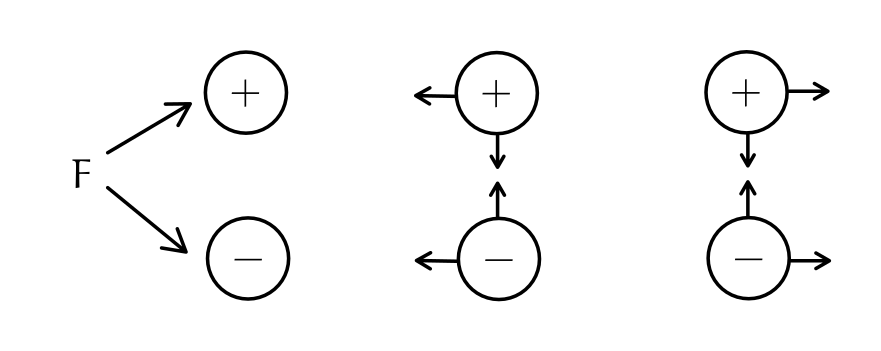
\includegraphics[width=0.8\textwidth]{tipi_carica}
  \caption{Tipi di carica}
\end{figure}
\begin{definition}[Carica elettrica]
  È chiamata \textbf{carica elettrica} \( q \) la proprietà che ha il corpo di esprimere
  la forza elettrostatica. Le proprietà di questa carica elettrica sono \textbf{indipendenti} dal
  meccanismo che l'ha generata, cioè può essere generata in modo diverso, ma ha sempre le
  stesse proprietà. Questo implica che la carica è \textbf{preesistente} in natura.
\end{definition}

\subsection{Materia}
L'atomo è formato da un nucleo centrale composto da protoni, carichi positivamente, e da
neutroni, senza carica. Intorno al nucleo si ha una regione in cui si ha la probabilità
di trovare un'altra particella, carica negativamente, chiamata elettrone.
\begin{figure}[H]
  \centering
  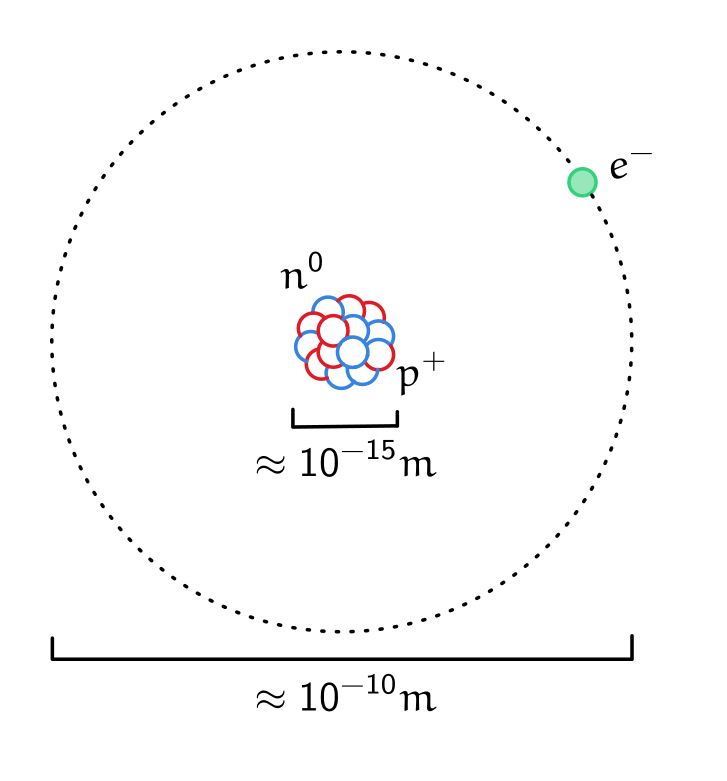
\includegraphics[width=0.6\textwidth]{atomo}
  \caption{Struttura dell'atomo}
\end{figure}
\noindent
La carica totale dell'atomo è nulla, quindi è \textbf{neutro} e
di conseguenza la carica del nucleo è uguale alla carica degli elettroni, per la precisione
il numero di protoni è uguale al numero di elettroni. \( Z \) è il numero atomico, cioè
il numero di protoni.

Elettrone e protone hanno, in modulo, la stessa carica:
\[
  |q_{e^{-}}| = q_{p^{+}}
\] 
L'elettrone è una \textbf{particella elementare}, indivisibile e la sua carica è detta
\textbf{carica elementare}, cioè la più piccola unità di carica osservabile e vale:
\[
  e^- = 1.6 \times 10^{-19}C
\] 
La \textbf{carica elettrica} in natura è quindi \textbf{quantizzata}, ovvero deve
essere un multiplo della carica dell'elettrone. Inoltre la carica non si può generare,
si può \textbf{solo trasferire}.

\begin{definition}[Legge di conservazione della carica]
  In un sistema isolato, cioè che non interagisce con altri sistemi, la carica totale 
  \( Q \) si conserva.
\end{definition}

\noindent
I componenti della materia hanno due comportamenti:
\begin{itemize}
  \item \textbf{Conduttore}: ad esempio il metallo, in cui gli elettroni sono liberi di
    muoversi
  \item \textbf{Dielettrico} (isolante): ad esempio il vetro, in cui le cariche non sono
    libere di muoversi, quindi vincolate, cioè non si riesce a strappare gli elettroni
    dall'atomo. Se si avvicina una carica positiva al dielettrico si avrà una deformazione
    delle cariche, ma non si ha una separazione di carica:
    \begin{figure}[H]
      \centering
      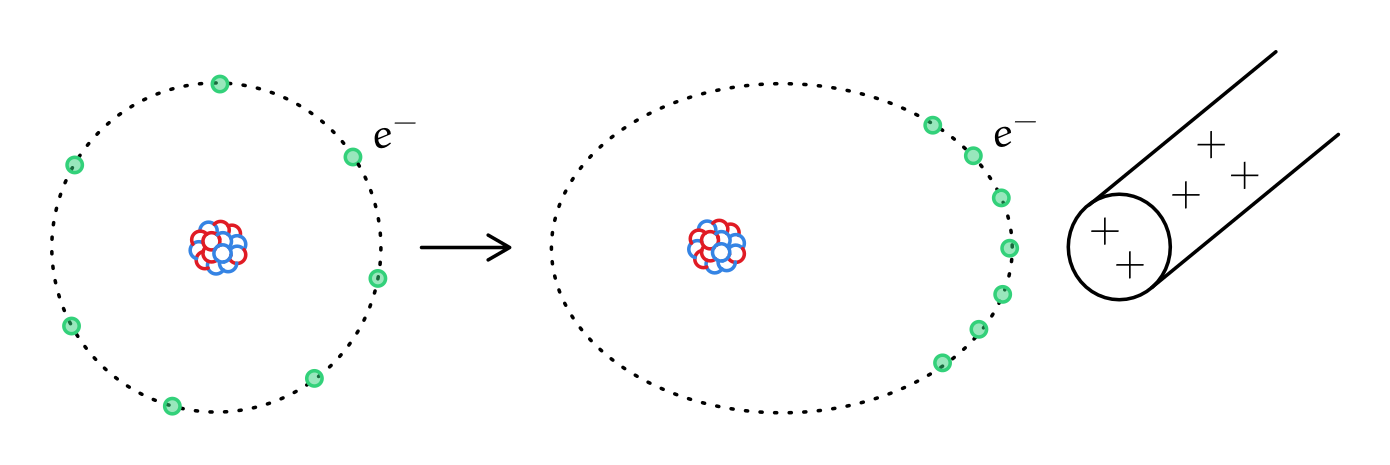
\includegraphics[width=1.0\textwidth]{dielettrico}
      \caption{Deformazione delle cariche}
    \end{figure}
    
\end{itemize}

\subsection{Elettrificazione}
L'elettrificazione è il trasferimento di carica da un corpo all'altro. Ci sono 3 
meccanismi di elettrificazione:
\begin{itemize}
  \item \textbf{Strofinio}:
    Si prende una bacchetta di vetro e un panno di lana e si strofina la bacchetta.
    La bacchetta, inizialmente, non è carica e meccanicamente con lo strofinio si strappano
    gli elettroni dagli atomi. La bacchetta diventa carica positivamente e il panno
    negativamente. Si avranno quindi le cariche \( q^+ \) della bacchetta e \( q^- \)
    del panno. Per la legge di conservazione della carica si ha:
    \[
      |q^-| = q^+
    \] 
    \begin{figure}[H]
      \centering
      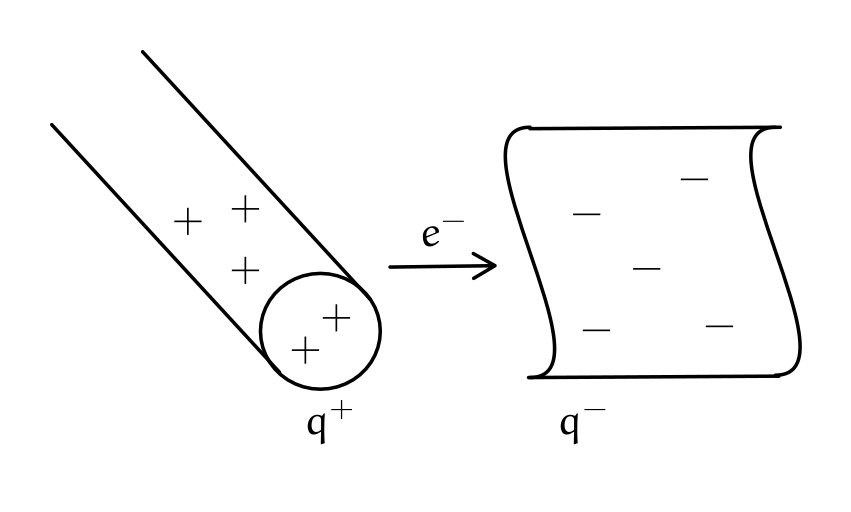
\includegraphics[width=0.7\textwidth]{strofinio}
      \caption{Strofinio}
    \end{figure}
  \item \textbf{Induzione elettrostatica}:
    Con la precedente bacchetta caricata positivamente si avvicina un oggetto metallico e
    si nota che le cariche negative \( -Q \)  del metallo si avvicinano il più possibile 
    alla bacchetta respingendo le cariche positive \( +Q \)  creando una 
    \textbf{separazione di carica per induzione}. La carica totale rimane nulla perchè 
    non sono migrati elettroni.
    \[
      |-Q| = +Q
    \] 
    \begin{figure}[H]
      \centering
      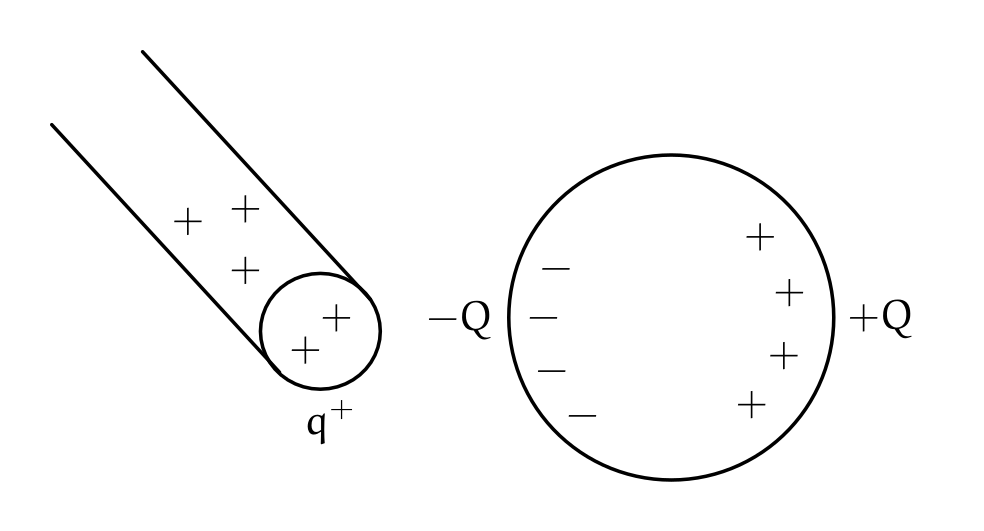
\includegraphics[width=0.7\textwidth]{induzione}
      \caption{Induzione elettrostatica}
    \end{figure}
    \noindent
    Se si allontana l'oggetto metallico si avrà una separazione meno potente.

    \vspace{1em}
    \noindent
    L'\textbf{elettroscopio} si usa per misurare la carica elettrica. È un oggetto metallico
    collegato a delle lamelle metalliche chiamate foglie:
    \begin{figure}[H]
      \centering
      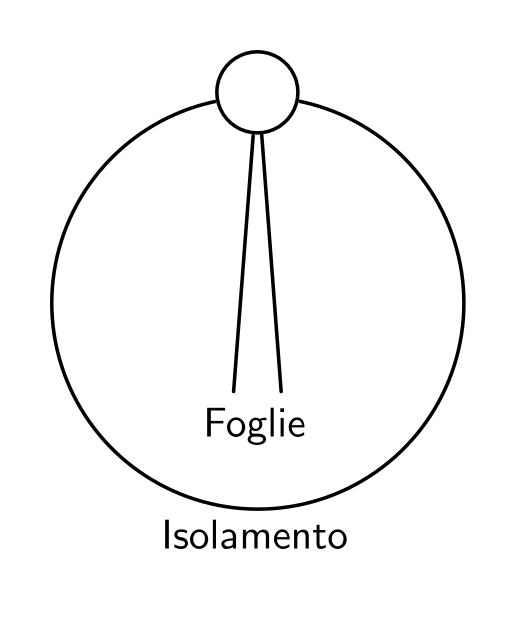
\includegraphics[width=0.4\textwidth]{elettroscopio_riposo}
      \caption{Elettroscopio}
    \end{figure}

    Si misura la carica avvicinando la bacchetta e si osserva la forza repulsiva tra le
    foglie dovuta alla repulsione tra le cariche positive della bacchetta e
    dell'elletroscopio:
    \begin{figure}[H]
      \centering
      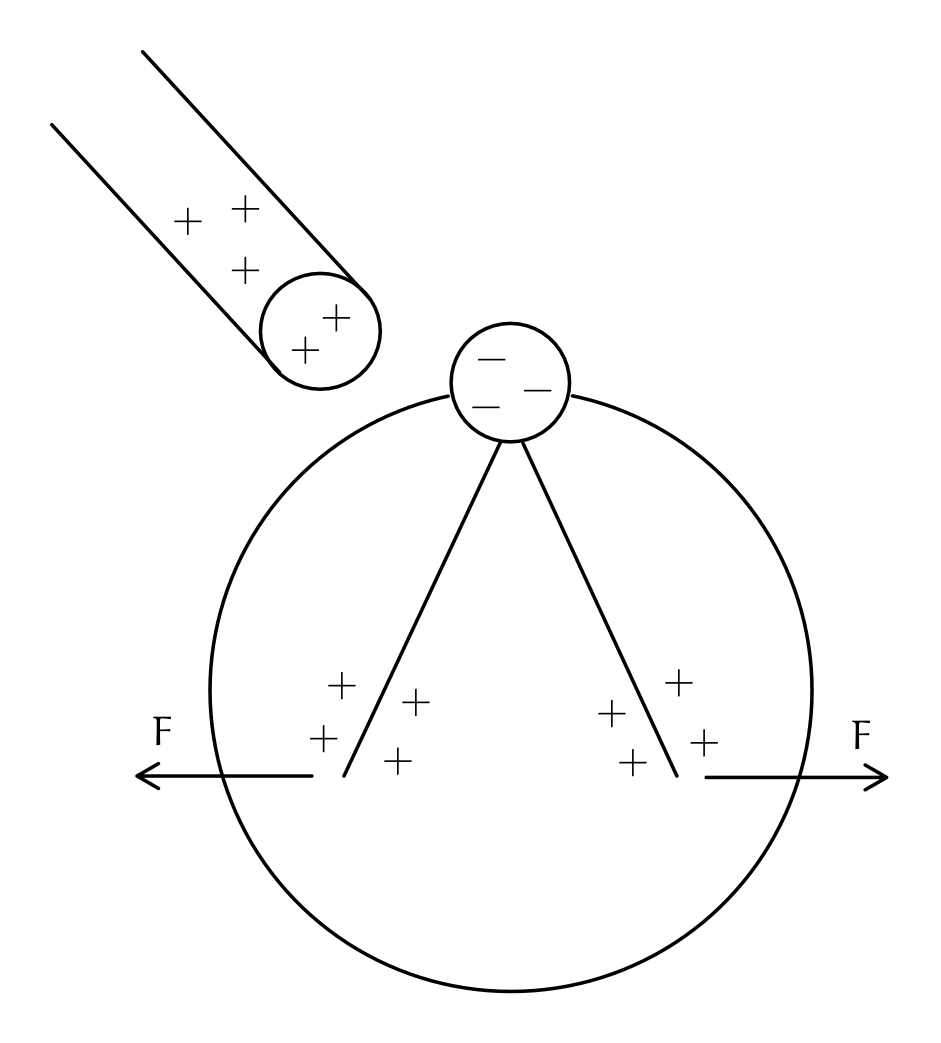
\includegraphics[width=0.5\textwidth]{elettroscopio_attivo}
      \caption{Elettroscopio durante una misurazione}
    \end{figure}
    Se si allontana la bacchetta la separazione delle foglie diminuisce.
  \item \textbf{Contatto}
    Se si prende un oggetto metallico caricato positivamente e si mette a
    contatto con un filo conduttore le cariche si sposteranno sul filo, elettrificandolo:
    \begin{figure}[H]
      \centering
      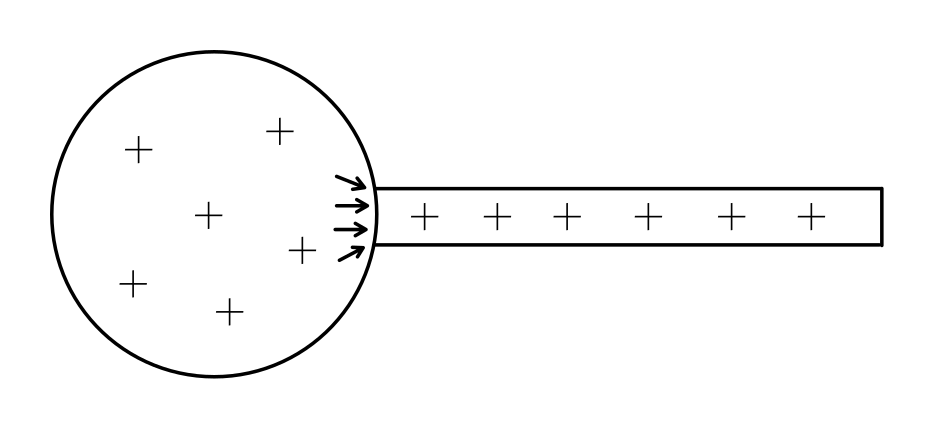
\includegraphics[width=0.7\textwidth]{contatto}
      \caption{Elettrificazione per contatto}
    \end{figure}
    Se si attacca il filo a terra l'oggetto si scarica perchè le cariche migrano verso
    la terra, cioè un conduttore immensamente più grande e quindi la carica si distribuisce
    su tutta la superficie della terra e sull'oggetto metallico rimane una carica
    \textbf{approssimativamente nulla}:
    \begin{figure}[H]
      \centering
      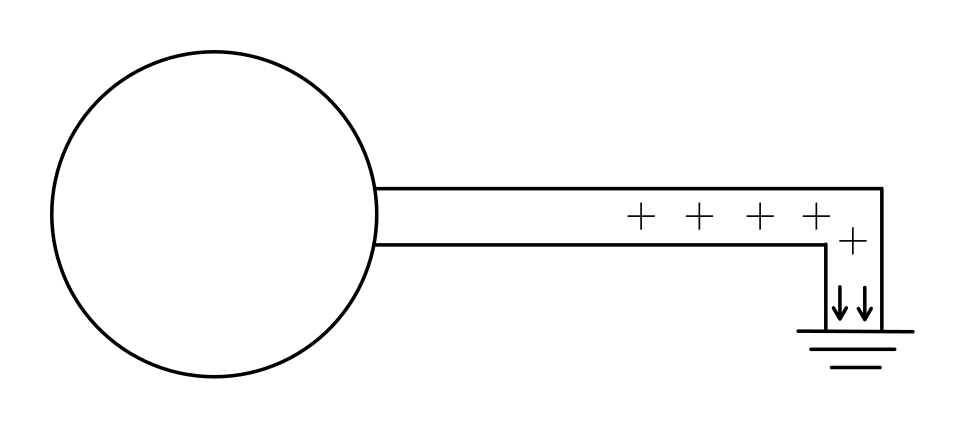
\includegraphics[width=0.7\textwidth]{contatto_terra}
      \caption{Scarica a terra}
    \end{figure}
\end{itemize}

\subsection{Elettrostatica nel vuoto}
\textbf{Fatti sperimentali}:

\vspace{1em}
\noindent
Si crea un esperimento che permette di osservare il fenomeno che si vuole modellare.
Si prende una bilancia di torsione formata da un filo torcente a cui è appesa un'asta 
con una carica \( q^+_1 \) su un'estremità. Se si avvicina una carica dello stesso
segno \( q^+_2 \) si osserva che viene applicata una forza repulsiva \( \vec{F}_{\text{el}} \)
che fa torcere il filo con un momento torcente:
\[
  \tau_{\text{filo}} = (k \theta) = \tau_{\text{el}} = \vec{d} \times \vec{F}
\]
\begin{figure}[H]
  \centering
  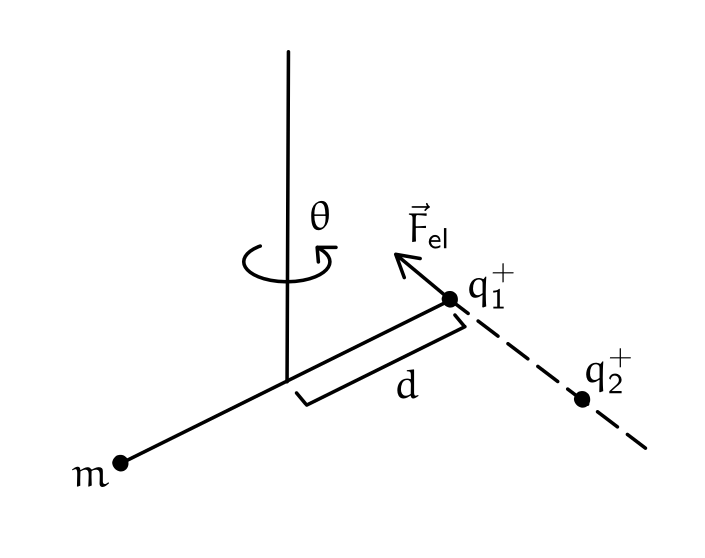
\includegraphics[width=0.7\textwidth]{bilancia_torsione}
  \caption{Bilancia di torsione}
\end{figure}
\subsubsection{Interazione di Coulomb}
Dai fatti sperimentali si nota che il modulo della forza è proporzionale al prodotto
delle cariche e inversamente proporzionale al quadrato della distanza tra le cariche:
\[
  | F_{\text{el}} | = k \frac{q_1 q_2}{r^2}
\] 
Si osserva anche che la forza elettrica \( F_{\text{el}} \) è una forza \textbf{centrale},
cioè la forza è diretta lungo la retta che congiunge le due cariche.

\( k \) è la costante di Coulomb e vale:
\[
  k = \frac{1}{4 \pi \varepsilon_0}
\]
dove \( \varepsilon_0 \) è la costante dielettrica del vuoto.
L'unità di misura della carica è il Coulomb:
\[
  [q] = C
\] 

\vspace{1em}
\noindent
Consideriamo la terna cartesiana con due cariche positive \( q^+_1 \) e \( q^+_2 \)
descritte dai raggi vettori \( \vec{r}_1 \) e \( \vec{r}_2 \). Sulla carica \( q^+_2 \) 
viene applicata una forza \( \vec{F}_{12} \) 
\begin{figure}[H]
  \centering
	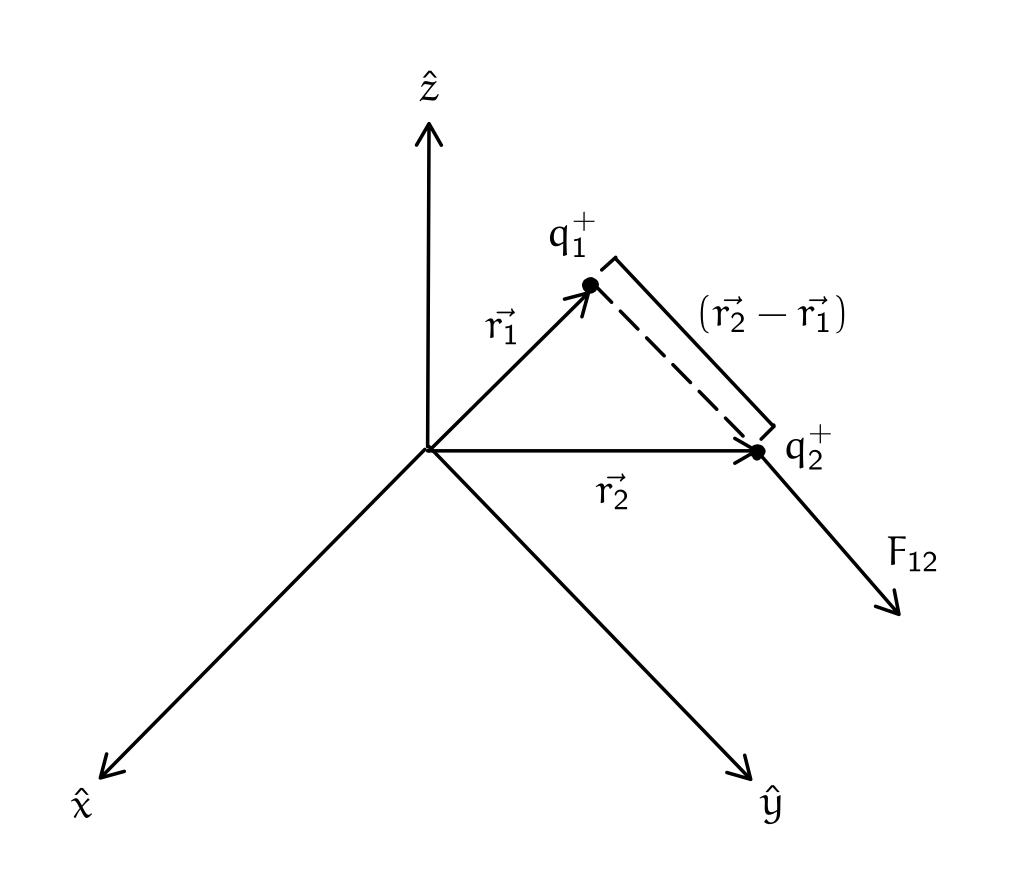
\includegraphics[width=0.7\textwidth]{forza_elettromagnetica}
  \caption{Forza elettromagnetica}
\end{figure}

\noindent
Notazione: 
\begin{itemize}
  \item 
    Chiamo il vettore che va da \( \vec{r}_1 \) a \( \vec{r}_2 \) \( \vec{r}_{12} \).

  \item 
    Il versore è indicato con \( \hat{r} \) e rappresenta il vettore unitario:
    \[
      \hat{r} = \frac{\vec{r}}{|\vec{r}|}
    \] 
\end{itemize}


\vspace{1em}
\noindent
Calcoliamo la forza \( \vec{F}_{12} \) che agisce su \( q^+_2 \) da \( q^+_1 \):
\[
  \vec{F}_{12} = \frac{1}{4 \pi \varepsilon_0} \frac{q_1 q_2}{\left( \vec{r}_{2}
    - \vec{r}_1 \right)^2} \frac{\left( \vec{r}_{2} - \vec{r}_1 \right)}{|\vec{r}_{2}
  - \vec{r}_1|} = 
  \frac{1}{4 \pi \varepsilon_0} \cdot \frac{q_1 q_2}{r_{12}^2} \cdot \hat{r}_{12} \quad [N]
\] 

\subsubsection{Sistema di più cariche}
Con più cariche si osserva che vale il principio di sovrapposizione, cioè due fenomeni
si sommano in modo lineare; e vale la terza legge di Newton, cioè l'azione-reazione
\( \left( \vec{F}_{12} = - \vec{F}_{21} \right)  \).

Consideriamo un sistema discreto con \( n \) cariche \( q_1, q_2, \ldots, q_n \) e osserviamo
la carica \( q_0 \). Ognuna di queste cariche sarà descritta dal suo raggio vettore.
\begin{figure}[H]
  \centering
  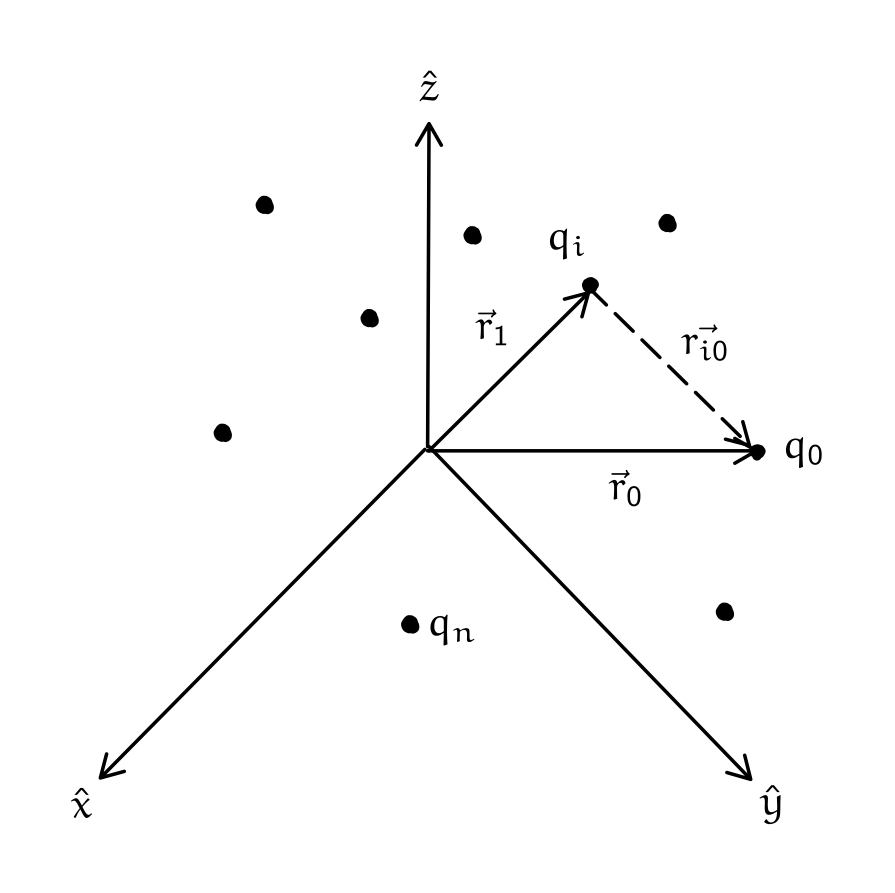
\includegraphics[width=0.7\textwidth]{forza_elettromagnetica_piu_cariche}
  \caption{Forza elettromagnetica con più cariche}
\end{figure}
\noindent
La forza che la carica \( q_i \) agisce su \( q_0 \) è:
\[
  \vec{F}_{i0} = \frac{q_i q_0}{4 \pi \varepsilon_0} \cdot \frac{\hat{r}_{i0}}{r_{i0}^2}
\] 
dove \( \vec{r}_{i0} = \vec{r}_0 - \vec{r}_i \).

Applichiamo questa formula osservando una ad una tutte le cariche come fatto per \( q_0 \)
per calcolare la forza totale applicata sulla carica \( q_0 \):
\[
  \vec{F}_{\text{tot}} = \sum_{i=1}^{n} \frac{q_i q_0}{4 \pi \varepsilon_0} \cdot 
  \frac{\hat{r}_{i0}}{r_{i0}^2} \quad \left[ N \right]
\] 
Questa forza ha direzione uguale alla somma delle forze.

\vspace{1em}
\noindent
Un'informazione si propaga con una \textbf{velocità finita}, cioè non istantaneamente. La
velocità massima di propagazione è la velocità della luce \( c \) e vale:
\[
  c = 3 \times 10^8 \, \frac{m}{s}
\]
Consideriamo lo stesso sistema di cariche, ma con la carica \( q_0 \) spostata ad una
distanza molto lontana e consideriamo le altre cariche come cariche che si muovono.
Si osserva che le cariche che si muovono cambiano il valore della forza 
\( \vec{F}_{\text{tot}} \) e dalla formula si vede che la forza cambia istantaneamente, 
ma in realtà la forza viene trasmessa dopo un tempo di propagazione (che la formula non 
tiene in considerazione).

Questa problematica si risolve con il concetto di \textbf{campo elettrostatico}.

\subsubsection{Campo elettrostatico}
Dalla formula della forza elettrostatica si può notare che la forza è proporzionale
alla carica osservata \( q_0 \):
\[
  \vec{F}_{\text{tot}} = \sum_{i=1}^{n} \frac{q_i q_0}{4 \pi \varepsilon_0} \cdot
  \frac{\hat{r}_{i0}}{r_{i0}^2} \propto q_0
\] 
Quindi la forza è proporzionale alla carica osservata e dalla distanza di questa carica:
\[
  \vec{F} = q_0 \vec{E} \left( \vec{r}_0 \right) 
\] 
Dove \( \vec{E} \) è il \textbf{campo elettrostatico} \textbf{posizionato in } \( r_0 \)
della carica osservata \( q_0 \).

\vspace{1em}
\noindent
Prendiamo in considerazione il seguente sistema in cui la particella \( Q \) è la
\textbf{sorgente di campo} e la particella \( q \) è la \textbf{carica di prova}:
\begin{figure}[H]
  \centering
  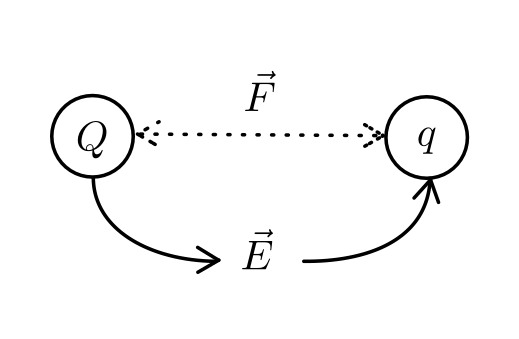
\includegraphics[width=0.6\textwidth]{campo_elettrostatico}
  \caption{Campo elettrostatico}
\end{figure}
\[
    \vec{F} = q \vec{E} \left( \vec{r} \right)
\] 
\[
  \vec{E} \left( r \right) = \frac{\vec{F}}{q}
\] 
Questa è la \textbf{definizione operativa} di campo, cioè serve una carica di prova per
misurare il campo.

\begin{definition}
  Il campo di una singola carica puntiforme \( Q \), posizionata per comodità nell'origine,
  considerata una particella di test \( q \) ad una distanza \( \vec{r} \) è definito come:
  \[
    \vec{E}( \vec{r} ) = \frac{Q}{4 \pi \varepsilon_0} \cdot \frac{\hat{r}}{r^2}
    \quad \left[ \frac{N}{C} \right]
  \] 
  \begin{figure}[H]
    \centering
    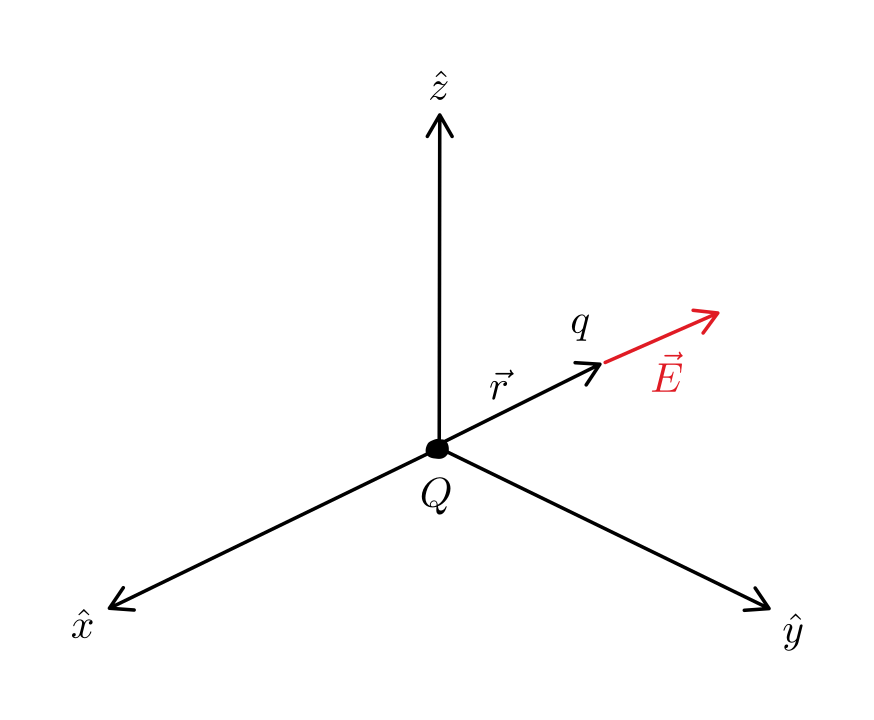
\includegraphics[width=0.6\textwidth]{campo_elettrostatico_def}
    \caption{Campo elettrostatico}
  \end{figure}
\end{definition}
\begin{definition}
  Il campo di un sistema discreto di \( n \) cariche \( q_1, q_2, \ldots, q_n \) è definito
  come:
  \[
    \vec{E} \left( \vec{r} \right) = \frac{1}{4 \pi \varepsilon_0} \sum_{i=1}^{n}
    \frac{q_i}{r_i^2} \cdot \hat{r}_i \quad \left[ \frac{N}{C} \right]
  \] 
  per il \textbf{principio di sovrapposizione}.
  \begin{figure}[H]
    \centering
    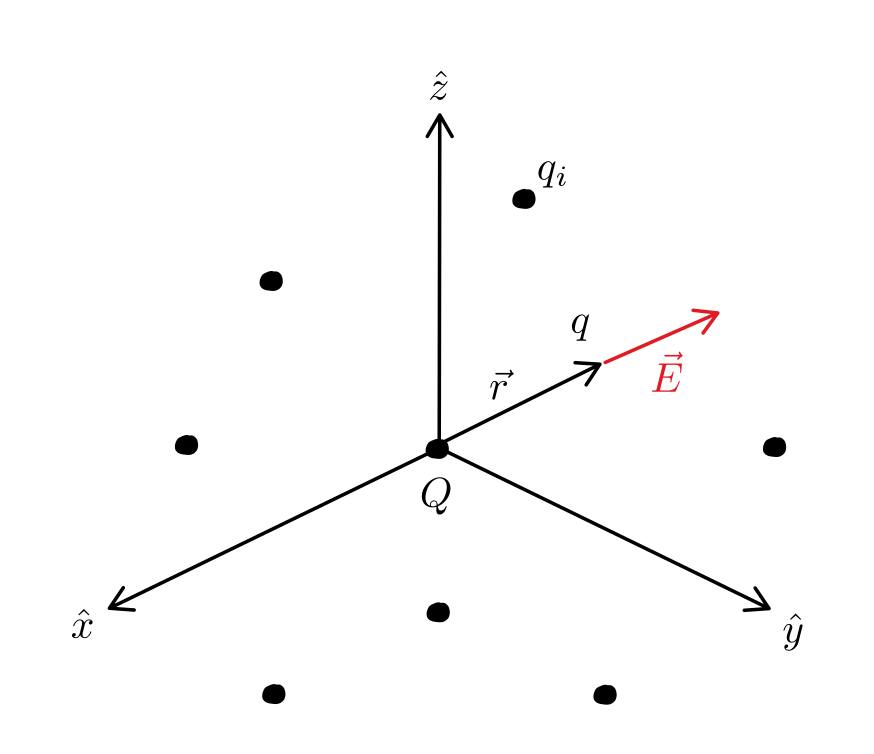
\includegraphics[width=0.6\textwidth]{campo_elettrostatico_def_piu_cariche}
    \caption{Campo elettrostatico con più cariche}
  \end{figure}
\end{definition}

\vspace{1em}
\noindent
\begin{define}
  Il \textbf{lavoro elementare} è definito come:
  \[
    dL = \vec{F} \cdot \vec{dl}
  \] 
  dove \( \vec{dl} \) è il vettore spostamento.
  \begin{itemize}
    \item Il lavoro non dipende dal percorso, ma solo dai punti di inizio e fine.
    \item Il lavoro in un percorso chiuso è nullo:
      \[
        \oint \vec{dl} = 0
      \] 
    \item Esiste una funzione di stato \( U \) tale che il lavoro per andare da \( A \) 
      a \( B \) è uguale al negativo del lavoro per andare da \( B \) a \( A \):
      \[
        \exists U \;|\; L_{AB} = - \Delta U
      \] 
      dove \( U \) è l'\textbf{energia potenziale}.
  \end{itemize}
\end{define}

\subsection{Energia potenziale elettrostatica}
La \textbf{forza elettrostatica} \( \vec{F}_{\text{el}} \) è una forza 
\textbf{conservativa}, cioè il lavoro per spostare una carica da un punto \( A \) a un 
punto \( B \) è indipendente dal percorso e dipende solo dai punti di inizio e fine.

Per calcolare il lavoro per spostare una carica \( q \) da un punto \( A \) a un punto \( B \)
si usa la seguente formula:
\[
  \begin{aligned}
    L_{AB} &= \int_{A}^{B} \vec{dL} = \int_{\text{curva}} \frac{1}{4 \pi \varepsilon_0}
    \frac{Qq}{r^2} \cdot \underbrace{\hat{r} \cdot \vec{dl}}_{dr}\\
           &= \frac{Qq}{4 \pi \varepsilon_0} \int_{r_A}^{r_B} \frac{dr}{r^2}\\
           &= \frac{Qq}{4 \pi \varepsilon_0} \left( - \frac{1}{r} \right) \Big|_{r_A}^{r_B}\\
           &= \frac{Qq}{4 \pi \varepsilon_0} \left( - \frac{1}{r_B} + \frac{1}{r_A} \right)\\
           &= - \Delta U
  \end{aligned}
\] 
dove \( U \) è l'\textbf{energia potenziale elettrostatica}:
\[
  U = \frac{Qq}{4 \pi \varepsilon_0} \cdot \frac{1}{r} + \text{costante} \quad [J]
\] 
\begin{figure}[H]
  \centering
  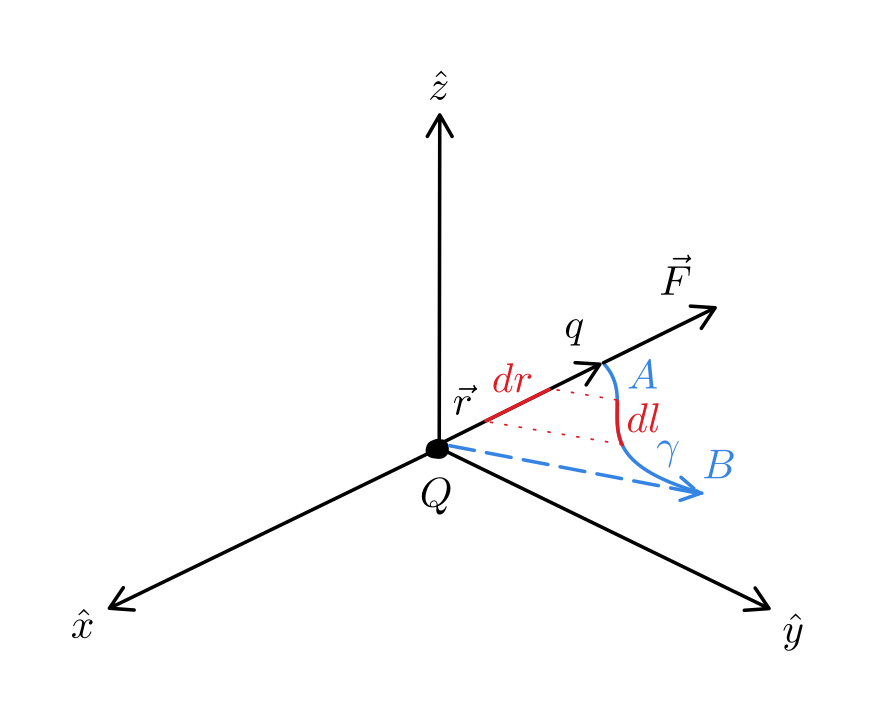
\includegraphics[width=0.7\textwidth]{energia_potenziale}
  \caption{Energia potenziale}
\end{figure}

\vspace{1em}
\noindent
Se poniamo l'energia all'infinito uguale a 0, allora \( U \) è il lavoro che fa il
campo (la forza elettrostatica) per allontanare una particella all'infinito, cioè per
distruggere il sistema:
\[
  U_{- \infty} = 0 \to U = \frac{Qq}{4 \pi \varepsilon_0 r} = - \left( U_{\infty} - U_r \right) 
\] 
\begin{itemize}
  \item Con cariche uguali l'energia è positiva perchè la forza è repulsiva e si allontana
    la carica verso l'infinito.
  \item Con cariche opposte l'energia è negativa perchè la forza è attrattiva e si avvicina
    la carica, allontanandosi dall'infinito.
\end{itemize}

\subsection{(Campo) Potenziale elettrostatico}
Dalla forza abbiamo definito l'equivalente, ma sottoforma di campo:
\begin{figure}[H]
  \centering
  \begin{tikzpicture}
    \node (f) {$\vec{F}$};
    \node[right=of f] (e) {$\vec{E} = \frac{\vec{F}}{q}$};

    \draw[->] (f) -- (e);
  \end{tikzpicture}
\end{figure}
\noindent
Si può definire un campo anche per l'energia potenziale:
\begin{figure}[H]
  \centering
  \begin{tikzpicture}
    \node (f) {$\vec{F}$};
    \node[right=of f] (e) {$\vec{E}$};
    \node[below=of f] (u) {$\Delta U$} 
      node at (u.south) [below,align=center,scale=0.7] {Energia\\elettrostatica};
    \node[below=of e] (v) {$\Delta V$} 
      node at (v.south) [below,align=center,scale=0.7] {Campo\\potenziale};


    \draw[->] (f) -- (e);
    \draw[->] (u) -- (v);
    \draw[->] (f) -- (u);
    \draw[->,dashed] (e) -- (v);
  \end{tikzpicture}
\end{figure}

\begin{definition}
  Il campo potenziale è definita come la differenza di energia di una carica \( q \) 
  unitaria:
  \[
    V(F) := \Delta V_{AB} = \frac{\Delta U}{q} \quad \left[ V \right]
  \] 
  L'unità di misura è il Volt.

  \vspace{1em}
  \noindent
  Quindi come \( \Delta U_{AB} = - \int_A^B \vec{F} \; dl \), così si avrà:
  \[
    \Delta V_{AB} = V_B - V_A = - \int_{\underset{\gamma}{A}}^B \vec{E} \; dl \quad \left[ V \right]
  \] 
  Di conseguenza il lavoro sulla carica \( q \) è:
  \[
    L_q = - q \Delta V \quad \left[ J \right]
  \] 
\end{definition}

\subsubsection{Calcolo del potenziale}
\( V(\vec{r}) \) è un campo definito a meno di una costante (come l'energia), ma si
sceglie un punto di riferimento (uno \textbf{zero}) che chiamiamo ad esempio \( \vec{r}_0 \)
e poniamo \( V(\vec{r}_0) = V_0 \). Successivamente si calcola il potenziale come
\( V(\vec{r}) - V(\vec{r}_0)\):
\[
\begin{cases}
  V(\vec{r_0}) = V_0 \to = 0\\
  V(\vec{r}) - V_0 = - \int_{\vec{r}_0}^{\vec{r}} \vec{E} \; dl
\end{cases}
\] 
Si calcola quindi il campo prendendo come punto di riferimento il punto \( \vec{r}_0 \) 

\subsubsection{Potenziale della carica puntiforme}
Ricordando la definizione di campo elettrostatico:
\[
  \vec{E} = \frac{Q}{4 \pi \varepsilon_0} \cdot \frac{\hat{r}}{r^2}
\] 
Il potenziale si calcola come:
\[
  \begin{aligned}
    V(\vec{r}) - V_0 &= - \int_{\vec{r}_0}^{\vec{r}} \vec{E} \; dl \\
                     &= - \int_{\vec{r}_0}^{\vec{r}} \frac{Q}{4 \pi \varepsilon_0}
                     \cdot \frac{\hat{r}}{r^2} \cdot  dl \\
                     &= - \frac{Q}{4 \pi \varepsilon_0} \int_{r_0}^{r} \frac{dr}{r^2} \\
                     &= \frac{Q}{4 \pi \varepsilon_0 r} -
                     \frac{Q}{4 \pi \varepsilon_0 r_0} \quad \left[ V \right]
  \end{aligned}
\] 
dove \( r_0 \) è un punto di riferimento e \( V_0 \) è il potenziale in quel punto.

Si può prendere \( r_0 = \infty \), quindi \( V_\infty = 0 \) e si ottiene:
\[
  V(\vec{r}) = \frac{Q}{4 \pi \varepsilon_0 r} \quad \left[ V \right]
\] 

\subsubsection{Potenziale di più cariche}
Consideriamo un insieme di cariche discrete \( \{q_i\}_N \) vale il \textbf{principio
di sovrapposizione} anche per il potenziale ed esso è definito tramite il campo.
Gli operatori somma e integrale commutano e quindi si ottiene:
\[
  V_{\text{tot}} = \sum V_i
\] 
dove:
\[
  V_i = \frac{q_i}{4 \pi \varepsilon_0 |\vec{r} - \vec{r}_i|}
\] 
e quindi:
\[
  V_{\text{tot}}(\vec{r}) = \frac{1}{4 \pi \varepsilon_0} \sum \frac{q_i}{|\vec{r}-\vec{r}_i|}
\] 
\begin{figure}[H]
  \centering
  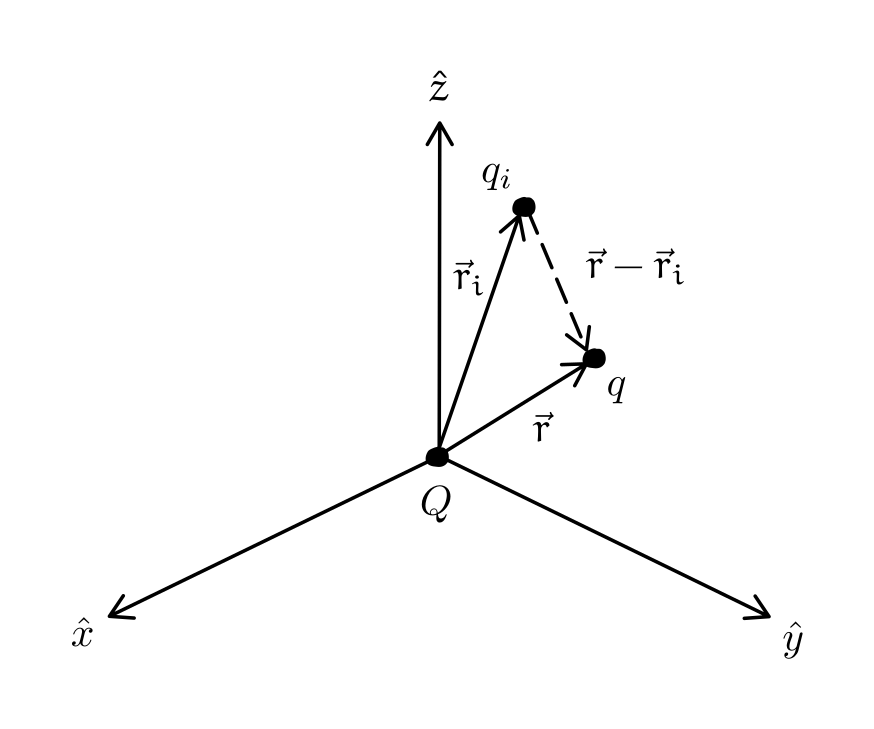
\includegraphics[width=0.6\textwidth]{potenziale_piu_cariche}
  \caption{Potenziale di più cariche}
\end{figure}
\noindent
In questo modo spostando l'origine degli assi il potenziale non cambia.

\vspace{1em}
\noindent
Se si avesse un volume tutte le sommatorie diventerebbero integrali:
\[
  V_{\text{tot}}(\vec{r}) = \frac{1}{4 \pi \varepsilon_0} \int \frac{dq}{|\vec{r} - \vec{r}_i|}
\] 

Abbiamo quindi che:
\begin{figure}[H]
  \centering
  \begin{tikzpicture}
    \node (f) {$\vec{F}$};
    \node[right=1.32cm of f] (e) {$\vec{E} = \frac{\vec{F}}{q_{\text{test}}}$};
    \node[below=of f] (u) {$\Delta U$} 
      node at (u.south) [below,align=center,scale=0.7] {Energia\\elettrostatica};
    \node[right=of u] (v) {$\Delta V = \frac{\Delta U}{q_{\text{test}}}$} 
      node at (v.south) [below,align=center,scale=0.7] {Campo\\potenziale};

    \node[below=1.1cm of u] (lu) {$L_q = - \Delta U$};
    \node[below=of v] (lv) {$L_q = -q \Delta V$};


    \draw[->] (f) -- (e);
    \draw[->] (u) -- (v);
    \draw[->] (f) -- (u) node[midway,left,scale=0.7] {conservativo};
    \draw[->] (e) -- (v) node[midway,right,scale=0.7] {conservativo};
    \draw[->] (lu) -- (lv);
  \end{tikzpicture}
\end{figure}
\noindent
La circuitazione in un percorso chiuso è nulla:
\begin{figure}[H]
  \[
    \oint_{\Gamma} \vec{E} \cdot dl = 0
  \] 
  \caption{Equazione di Maxwell}
\end{figure}
quindi \( \vec{E} \) è \textbf{conservativo}.

\subsection{Linee di campo}
Sono linee tangenti al campo elettrostatico \( \vec{E} \) in ogni punto e dirette
nel verso del campo. Hanno le seguenti caratteristiche:
\begin{itemize}
  \item Sono continue, quindi non si interrompono mai
  \item Escono dalle cariche positive e entrano nelle cariche negative
  \item Sono linee aperte, cioè non si chiudono mai

  \item In una carica positiva puntiforme sono radiali
    \begin{figure}[H]
      \centering
      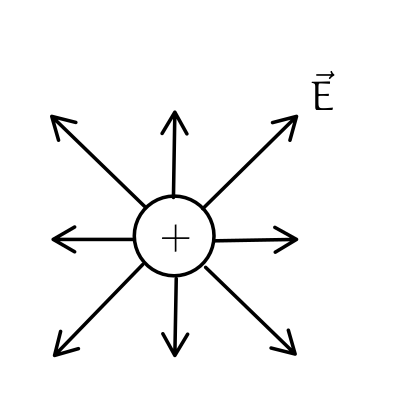
\includegraphics[width=0.3\textwidth]{linee_campo_positivo}
      \caption{Linee di campo su una carica positiva}
    \end{figure}

  \item In una carica negativa puntiforme sono radiali e entrano nella carica
    \begin{figure}[H]
      \centering
      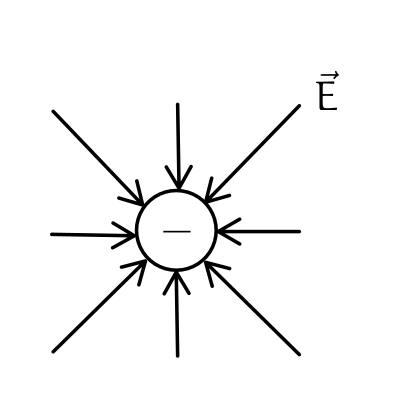
\includegraphics[width=0.3\textwidth]{linee_campo_negativo}
      \caption{Linee di campo su una carica negativa}
    \end{figure}

  \item Le cariche sono l'origine delle linee di campo, se si hanno delle linee chiuse
    vuol dire che non c'è una sorgente

  \item Le linee di campo non si intersecano mai
\end{itemize}

\subsection{Superfici equipotenziali}
Sono luoghi di punti (superficie bidimensionale) a potenziale costante:
\[
  V(\vec{r}) = \text{costante} \to \Delta V = 0 \to L = 0 \quad \text{sulla superficie}
\] 
Se il lavoro è nullo, allora la forza è perpendicolare alla superficie \( \vec{F} \perp \vec{dl} \).
Quindi le superfici equipotenziali sono perpendicolari al campo elettrico perchè:
\[
  \vec{F} = q \vec{E} \to \vec{F} \perp \vec{E}
\] 
Quindi si nota che per una carica puntiforme la superficie equipotenziale è una sfera.
Il campo elettrico punta sempre verso potenziali minori perchè il lavoro è positivo:
\begin{figure}[H]
  \centering
  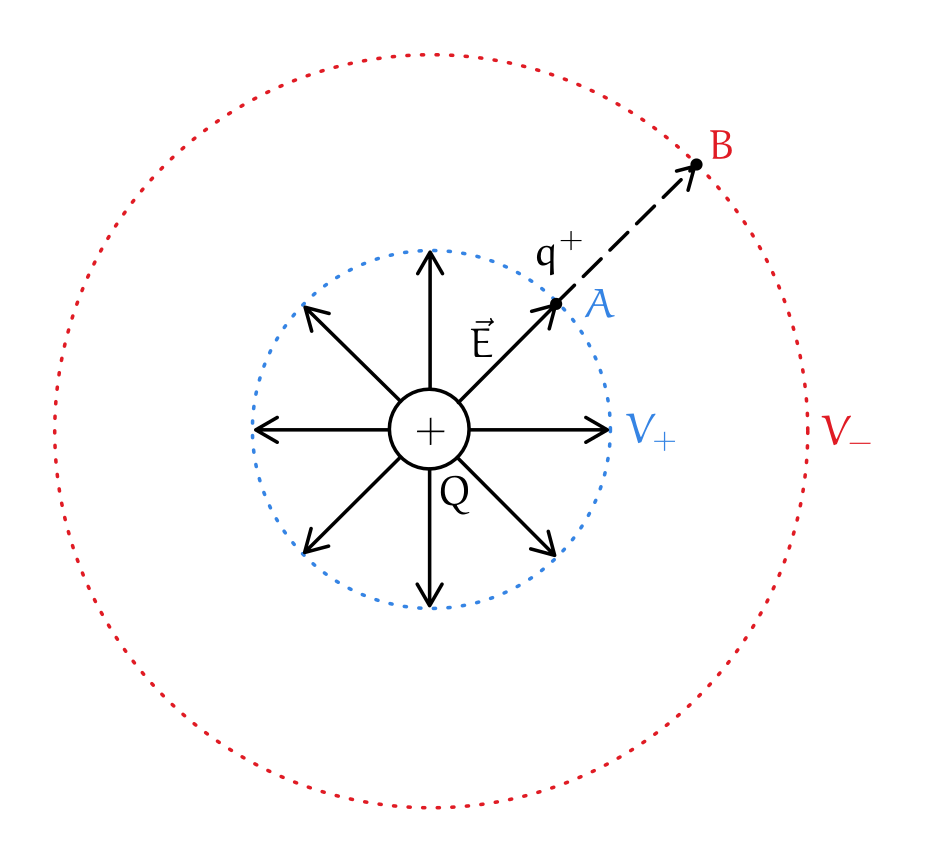
\includegraphics[width=0.8\textwidth]{superfici_equipotenziali}
  \caption{Superfici equipotenziali}
\end{figure}
\[
  L = -q^+ \left( V_B - V_A \right) > 0 \quad \text{con } V_B < V_A
\] 

\subsection{Teorema di Gauss}
Si può calcolare il campo elettrostatico \( \vec{E} \) di un'entità più complicata, come
ad esempio un filo, un cilindro ecc..., che presentano \textbf{situazioni di simmetria}.
Questo calcolo non viene fatto direttamente tramite integrali, ma tramite il \textbf{teorema
di Gauss}. Le simmetrie che analizziamo sono:
\begin{itemize}
  \item \textbf{Simmetria sfericha}: Un sistema \textbf{isotropo}, cioè che non varia in
    base alla direzione. Ad esempio una sfera, una carica puntiforme oppure un
    condensatore sferico.

  \item \textbf{Simmetria cilindrica}: Un sistema che non varia in base alla rotazione 
    intorno ad un asse. Ad esempio un cilindro \textbf{indefinito} (di lunghezza non 
    definita) oppure un filo.

  \item \textbf{Simmetria rispetto ad un piano}: Un sistema che non varia in base alla 
    traslazione lungo un piano.
\end{itemize}
Tutte queste sono geometrie in cui sono distribuite cariche e avranno una certa densità
di carica:
\begin{itemize}
  \item Carica puntiforme \( q \; \left[ C \right] \)
  \item Densità lineare \( \lambda \; \left[ \frac{C}{m} \right] \) per una linea
  \item Densità superficiale \( \sigma \; \left[ \frac{C}{m^2} \right] \) per una superficie
  \item Densità volumetrica \( \rho \; \left[ \frac{C}{m^3} \right] \) per un volume
\end{itemize}

\vspace{1em}
\noindent
\textbf{Osservazione}: Moltiplicare un campo per una superficie equivale a calcolare un
\textbf{flusso}, cioè contare le linee di campo per la superficie ortogonale. Se prendiamo
un campo di una carica puntiforme notiamo che al variare della distanza \( \vec{r} \) 
il valore del campo varia. Se invece moltiplichiamo il campo per la superficie di una 
sfera, si ottiene un flusso che è costante e non dipende da \( \vec{r} \):
\[
  \vec{E} = \frac{q \hat{r}}{4 \pi \varepsilon_0 r^2}
\] 
\[
  \vec{E} \cdot 4 \pi r^2 = \frac{q \hat{r}}{\cancel{4 \pi} \varepsilon_0 \cancel{r^2}}
  \cdot \cancel{4 \pi r^2} = \frac{q}{\varepsilon_0} \cdot \hat{r}
\] 

\begin{define}[Angolo piano]
  L'angolo solido \( d \alpha \) è definito come un elemento di linea \( dl \) di 
  circonferenza diviso per il raggio:
  \begin{figure}[H]
    \centering
    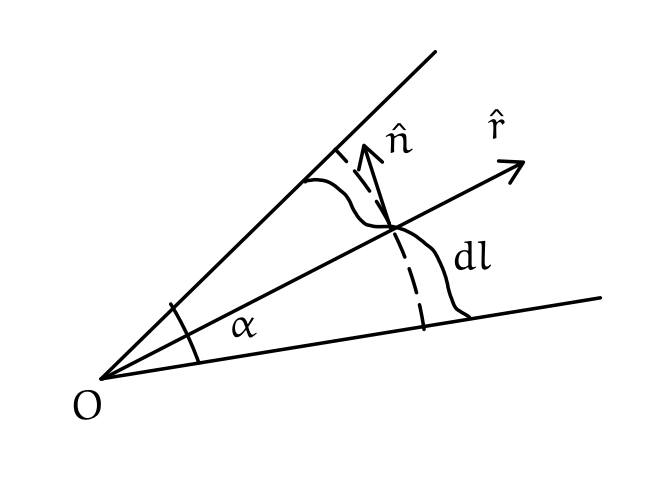
\includegraphics[width=0.4\textwidth]{angolo_piano}
    \caption{Angolo piano}
  \end{figure}
  \[
    d \alpha = \frac{\vec{dl} \cdot \hat{n} \cdot \hat{r}}{r}
  \] 
\end{define}
\begin{define}[Angolo solido]
  L'angolo solido \( d \Omega \) è definito come un elemento di superficie \( dS \) diviso
  per il raggio al quadrato:
  \begin{figure}[H]
    \centering
    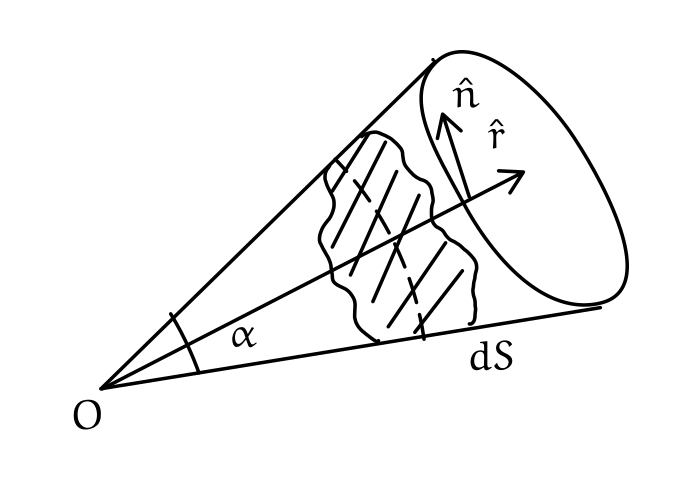
\includegraphics[width=0.4\textwidth]{angolo_solido}
    \caption{Angolo solido}
  \end{figure}
  \[
    d \Omega = \frac{dS \cdot \hat{n} \cdot \hat{r}}{r^2}
  \]
  
\end{define}

\subsubsection{Flusso del campo \texorpdfstring{\( \vec{E} \)}{E}}
Consideriamo una superficie con concavità verso il basso definita come la sua orientazione
\( \hat{n} \) (normale) e la sua area \( dS \).
\begin{figure}[H]
  \centering
  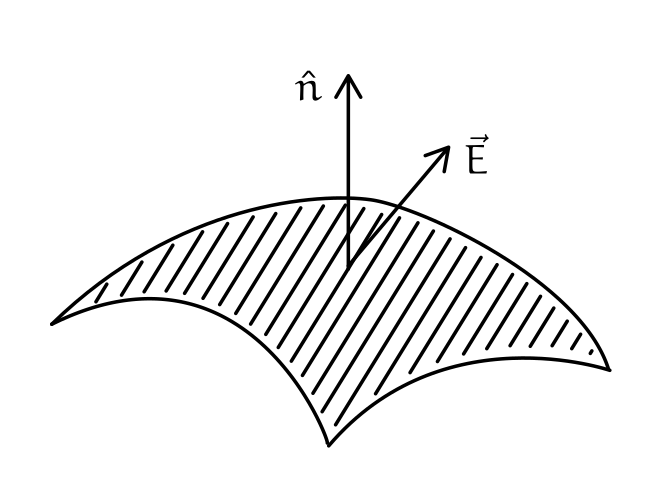
\includegraphics[width=0.6\textwidth]{superficie}
  \[
    d\vec{S} = \hat{n} \cdot dS
  \] 
  \caption{Superficie}
\end{figure}
\begin{definition}[Flusso elementare]
  Il flusso elementare \( d \Phi \) è definito come il prodotto scalare tra il campo
  e la superficie:
  \[
    d \Phi = \vec{E} \cdot d \vec{S} \quad \left[ V \cdot m \right]
  \] 

  \vspace{1em}
  \noindent
  Il flusso di una superficie si ottiene integrando:
  \[
    \Phi = \oint \vec{E} \cdot d \vec{S}
  \] 
  \begin{figure}[H]
    \centering
    \setkeys{Gin}{width=\linewidth}
    \begin{subfigure}{0.3\textwidth}
      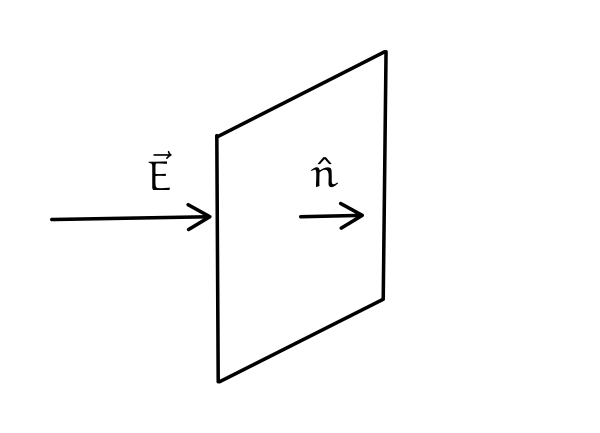
\includegraphics{flusso_positivo}
      \[
        d \Phi > 0
      \] 
      \caption{Flusso positivo}
    \end{subfigure}
    \hfil
    \begin{subfigure}{0.3\textwidth}
      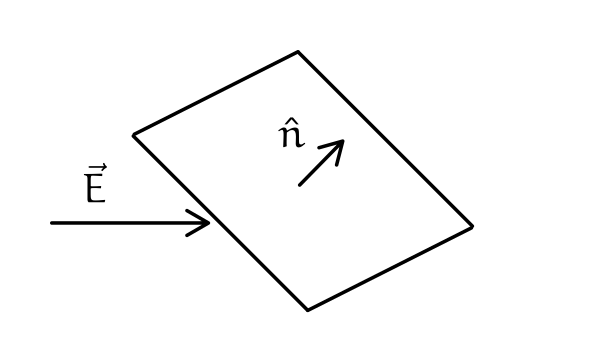
\includegraphics{flusso_generico}
      \[
       \Phi = \vec{E} \cdot \vec{S} \cos \theta
      \] 
      \caption{Flusso generico}
    \end{subfigure}
    \hfil
    \begin{subfigure}{0.3\textwidth}
      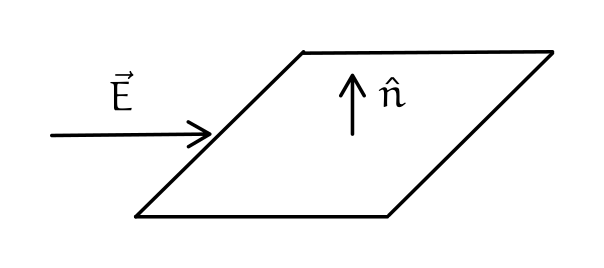
\includegraphics{flusso_nullo}
      \[
        \Phi = \vec{E} \cdot \vec{S} = 0
      \] 
      \caption{Flusso nullo}
    \end{subfigure}
    \caption{Esempi di flusso}
  \end{figure}
\end{definition}

\begin{example}
  Consideriamo una carica puntiforme \( q \) e una superficie \( dS \) 
  \begin{figure}[H]
    \centering
    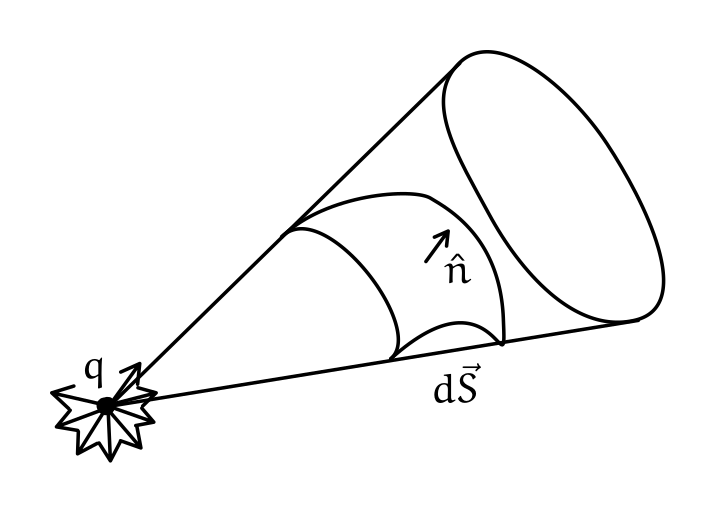
\includegraphics[width=0.5\linewidth]{flusso_puntiforme}
    \caption{Flusso di una carica puntiforme}
  \end{figure}
  Il flusso del campo elettrostatico è:
  \[
    d \Phi = \left( \vec{E} \cdot d\vec{S} \right) = \frac{q}{4 \pi \varepsilon_0} 
    \underbrace{\frac{\hat{r}}{r^2} \cdot d\vec{S}}_{d \Omega} = \frac{q}{4 \pi \varepsilon_0}
    d \Omega
  \] 
  Osserviamo che il flusso dipende solo da \( d \Omega \), cioè dall'angolo solido,
  e non dalla distanza \( r \) della superficie dalla carica.
\end{example}
\begin{example}
  Consideriamo una superficie chiusa:
  \begin{figure}[H]
    \centering
    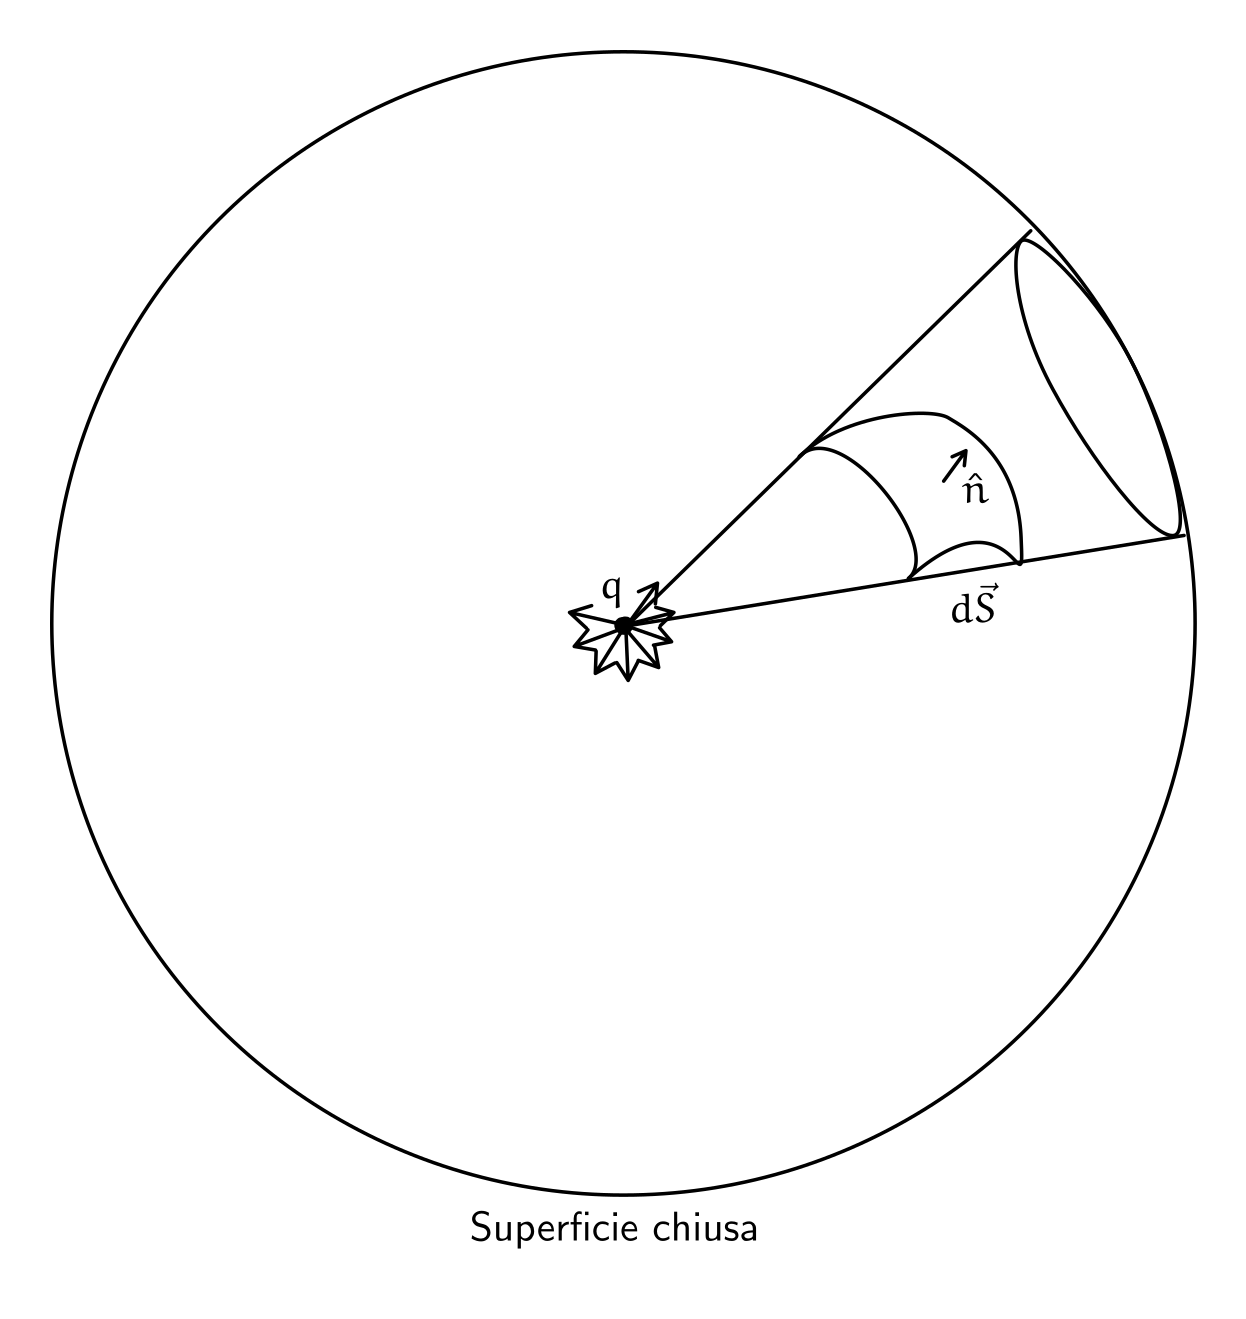
\includegraphics[width=0.7\linewidth]{flusso_superficie_chiusa}
    \caption{Flusso di una superficie chiusa}
  \end{figure}
  il flusso del campo elettrostatico è:
  \[
    \Phi = \oint \frac{q}{4 \pi \varepsilon_0} d \Omega = \frac{q}{4 \pi \varepsilon_0}
    \underbrace{\oint d \Omega}_{= 4 \pi} = \frac{q}{\varepsilon_0}
  \] 
  L'integrale su una superficie chiusa dell'angolo piano è uguale a \( 2 \pi  \),
  quindi l'integrale su una superficie chiusa dell'angolo solido è uguale a \( 4 \pi \).
\end{example}
Il flusso quindi non dipende dalla superficie. Questa è la dimostrazione del teorema
di Gauss.

\begin{theorem}[Teorema di Gauss]
  Il flusso \( \Phi(\vec{E}) \) del campo elettrico \( \vec{E} \) attraverso una
  superficie chiusa \textbf{qualsiasi} \( S \) è uguale alla somma delle cariche interne alla superficie
  diviso \( \varepsilon_0 \):
  \[
    \Phi (\vec{E}) = \underset{\text{superficie chiusa QUALUNQUE}}{\oint} \vec{E} \cdot d \vec{S} = \frac{Q_{\text{interne}}}{\varepsilon_0}
  \] 
  Le cariche esterne non contano perchè quando esse entrano nella superficie, ad un
  certo punto escono, quindi il flusso è nullo. Se all'interno della superficie c'è
  una sorgente (quindi cariche interne) esse non entrano mai perchè sono già dentro,
  quindi escono e il flusso è positivo.
\end{theorem}

\subsection{Applicazione del teorema di Gauss}
Siccome il teorema di Gauss dice che il flusso non dipende dalla superficie si prende
una superficie particolarmente simmetrica chiamata \textbf{superficie di Gauss} che
rende facilmente calcolabile il flusso, grazie al campo costante su tutta la superficie.
Per calcolare il campo \( \vec{E} \) siccome esso è costante e parallelo alla normale
(grazie alla superficie scelta) si può tirare fuori dall'integrale per ottenere un
prodotto tra l'incognita \( \vec{E} \) e un integrale geometrico.
\begin{figure}[H]
  \[
    \Phi (\vec{E}) = \vec{E} \cdot \oint_{\text{Sup}} d \vec{S} =
    \frac{Q_{\text{Interne}}}{\varepsilon_0}
  \] 
  \caption{Equazione di Maxwell}
\end{figure}
\subsubsection{Simmetria sferica}
Le caratteristiche necessarie sono:
\begin{itemize}
  \item Distribuzione di carica con simmetria sferica. Potrebbe essere una:
    \begin{itemize}
      \item Carica di volume \( \rho \)
        \begin{figure}[H]
          \centering
          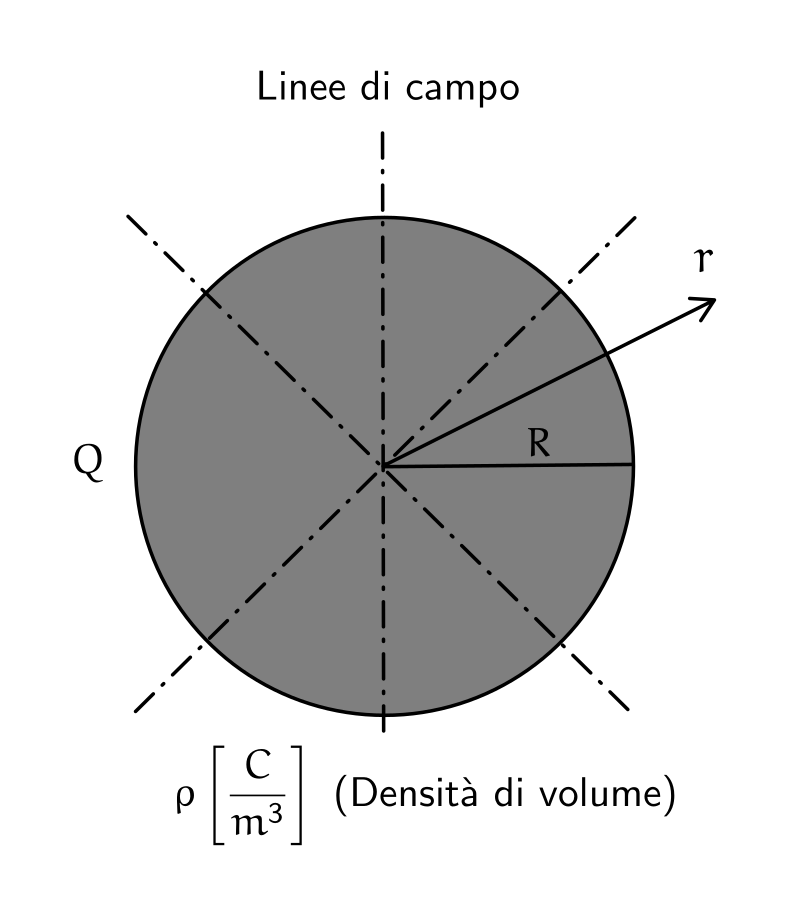
\includegraphics[width=0.5\textwidth]{simmetria_sferica_volume}
          \[
            Q = \rho \cdot \overbrace{\frac{4}{3}\pi R^3}^{\text{Volume sfera}}
            \quad \left[C\right]
          \] 
          \caption{Simmetria sferica di volume}
        \end{figure}
      \item Carica di superficie \( \sigma \)
        \begin{figure}[H]
          \centering
          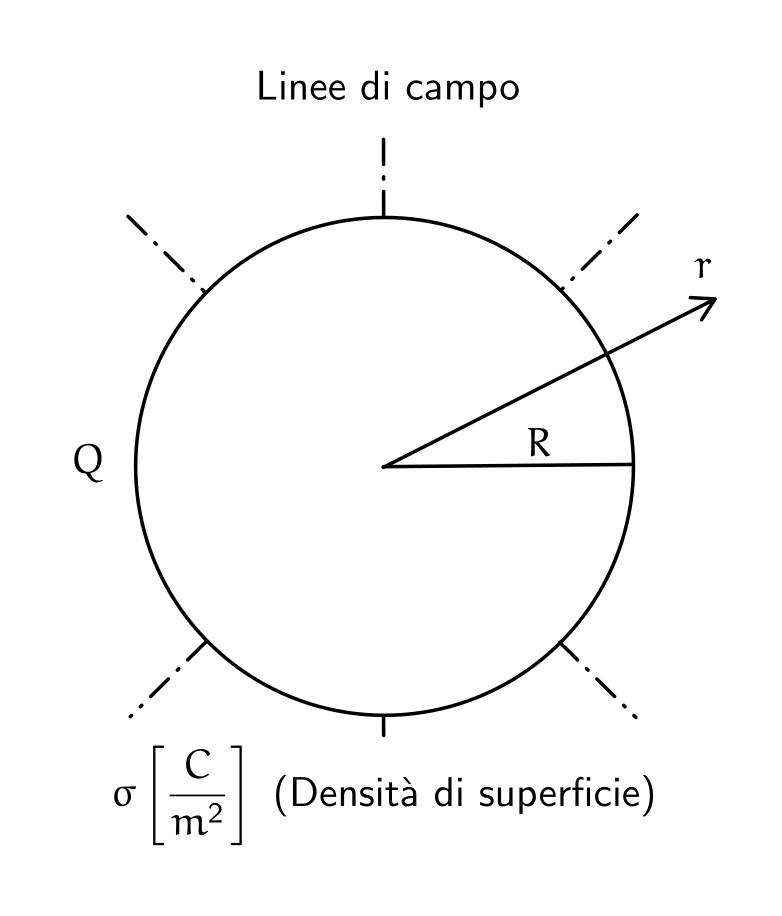
\includegraphics[width=0.5\textwidth]{simmetria_sferica_superficie}
          \[
            Q = \sigma \cdot \overbrace{4 \pi R^2}^{\text{Superficie sfera}}
            \quad \left[C\right]
          \] 
          \caption{Simmetria sferica di superficie}
        \end{figure}
    \end{itemize}
    Se la carica \( \{Q\} \) è a simmetria sferica, allora il campo \( \vec{E} \) sarà
    a simmetria sferica. Questo campo sarà \textbf{radiale} e dipenderà solo da \( \vec{r} \):
    \[
      \vec{E} = E(r) \hat{r}
    \] 
\end{itemize}

\begin{example}
  Consideriamo una carica positiva \( Q^+ \) distribuita su una superficie. L'obiettivo
  è quello di cercare una superficie di Gauss in cui il campo elettrico sia costante.
  Siccome dipende solo da \( r \) esso sarà costante solo nelle superfici sferiche \( S(r) \) 
  di raggio \( r \).
  \begin{figure}[H]
    \centering
    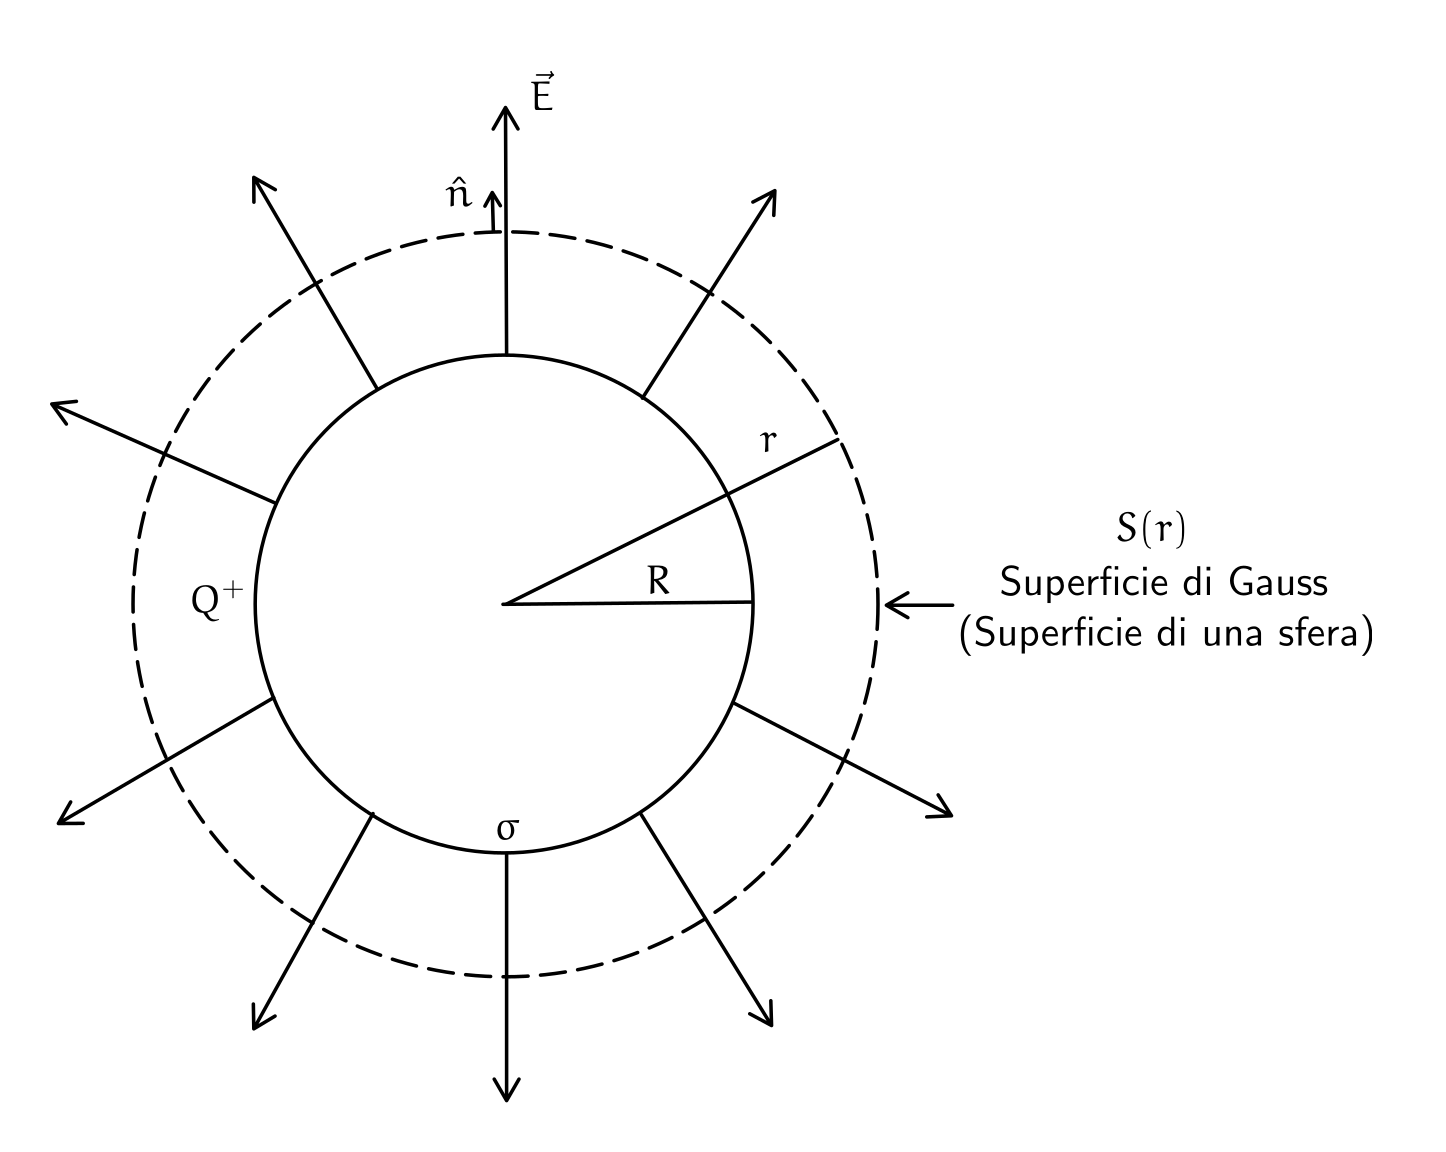
\includegraphics[width=0.9\textwidth]{carica_superficie_sferica}
    \caption{Carica distribuita su una superficie sferica}
  \end{figure}
  \[
    \begin{aligned}
      \Phi(\vec{E}) &= \oint_{S(r)} \vec{E} \cdot \hat{n} \cdot_{S(r)} dS\\
      &= \oint_{S(r)} E(r) dS\\
      &= E(r) \overbrace{\oint_{S(r)} dS}^{\text{Sup sfera}}\\
      &= E(r) \cdot 4 \pi r^2 = \frac{Q_{\text{int}}}{\varepsilon_0}
    \end{aligned}
  \]
  Dove:
  \[
    Q_{\text{int}} =
  \begin{cases}
    Q & \text{se } r \ge R \text{ (esterno)}\\
    0 & \text{se } r < R \text{ (interno)}
  \end{cases}
  \] 
  Quindi:
  \[
    E(r) = \begin{cases}
      \frac{Q}{4 \pi \varepsilon_0 r^2} & \text{se } r \ge R\\
      0 & \text{se } r < R
    \end{cases}
    \quad \left[ \frac{V}{m} \right]
  \] 
  In \( r = R \) il campo vale:
  \[
    E(R) = \frac{Q}{4 \pi \varepsilon_0 R^2} = \frac{\sigma}{\varepsilon_0}
  \] 
  Il grafico del campo elettrico è:
  \begin{figure}[H]
    \centering
    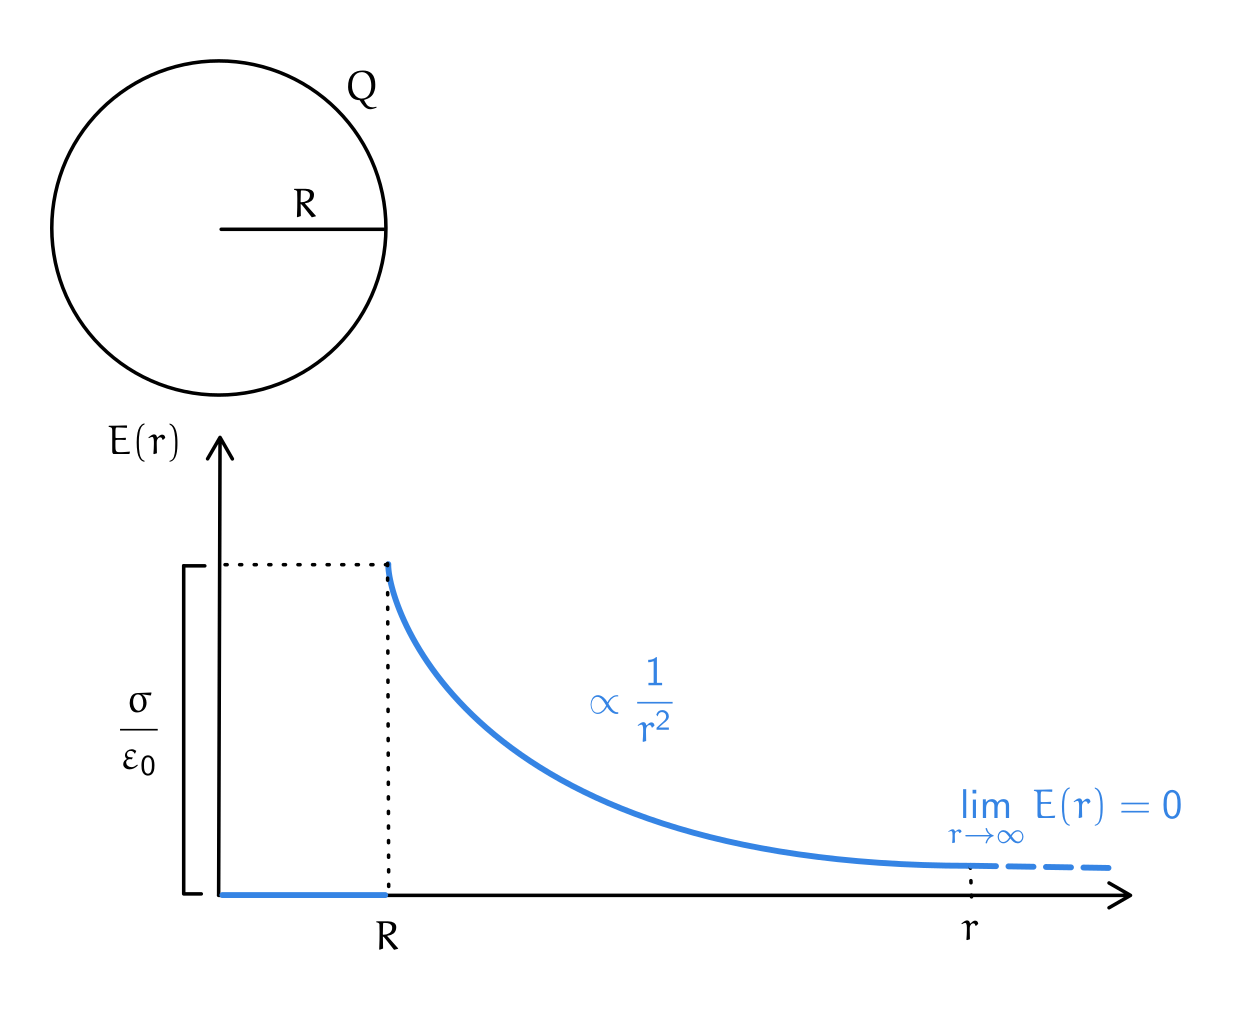
\includegraphics[width=0.9\textwidth]{grafico_superficie_sferica}
    \caption{Grafico del campo elettrico}
  \end{figure}
\end{example}
\begin{example}
  Consideriamo una carica positiva \( Q^+ \) distribuita su un volume. L'obiettivo è
  quello di cercare una superficie di Gauss in cui il campo elettrico sia costante.
  Siccome dipende solo da \( r \) esso sarà costante solo nelle sfere \( S(r) \) di raggio
  \( r \).
  \begin{figure}[H]
    \centering
    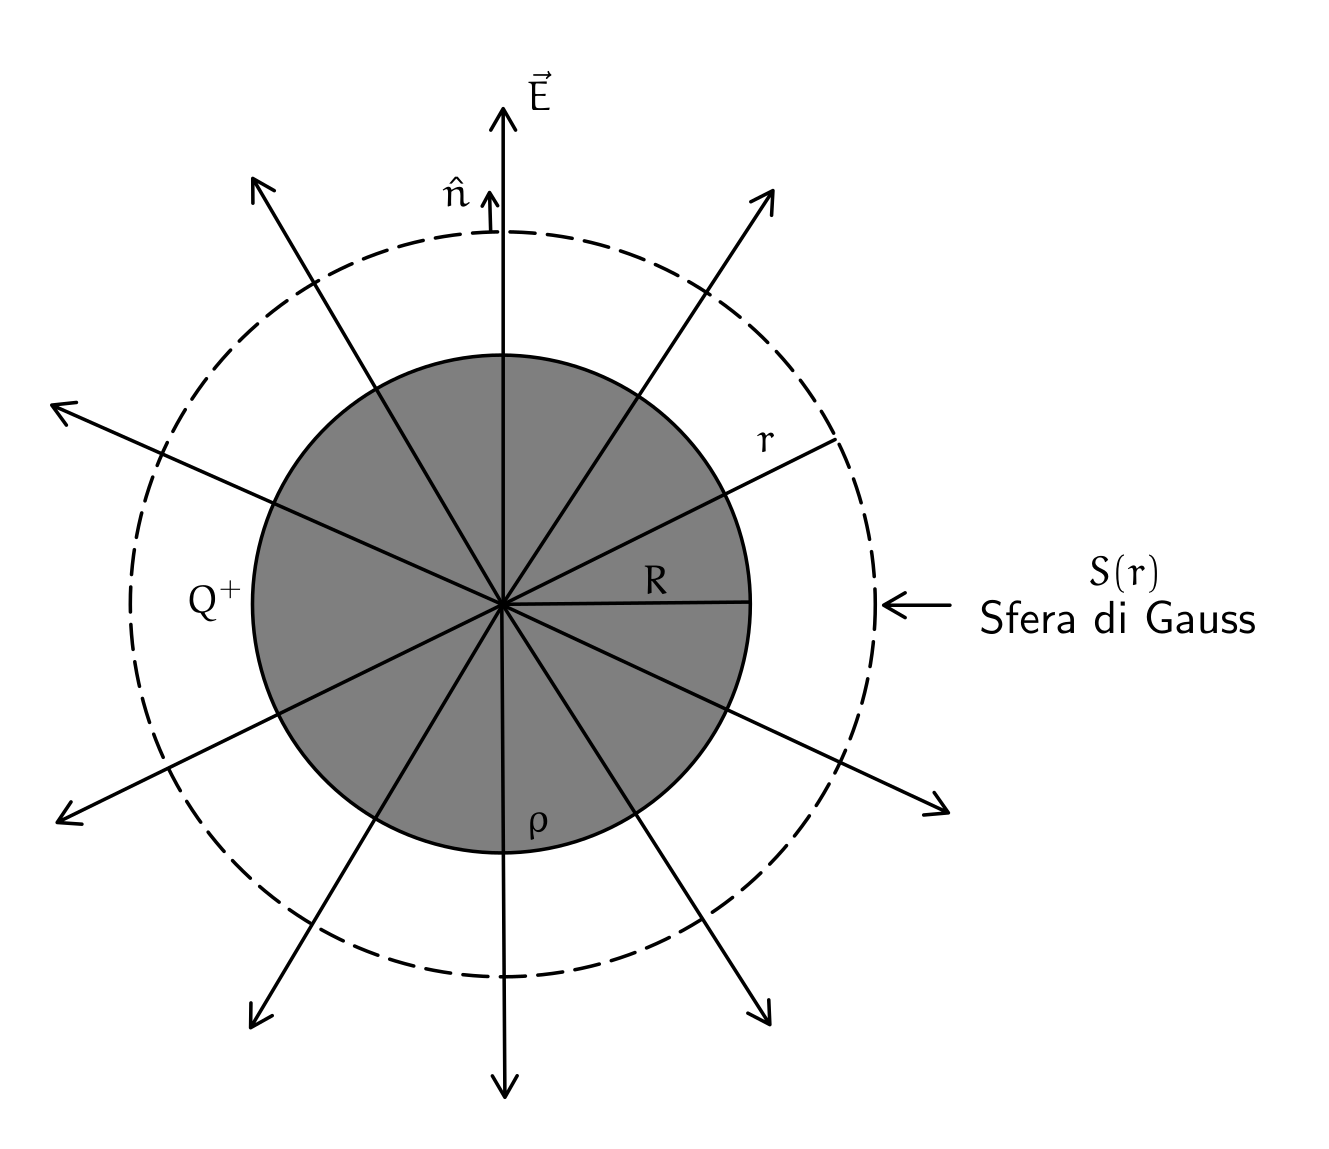
\includegraphics[width=0.9\textwidth]{carica_volume_sferico}
    \caption{Carica distribuita su un volume sferico}
  \end{figure}
  \noindent
  Siccome la sfea all'interno non è più vuota come nell'esempio precedente, ma è piena
  il valore di \( Q_{\text{int}} \) esterno rimane invariato, ma all'interno si ha:
  \[
    Q_{\text{Int}} = 
    \begin{cases}
      Q & \text{se } r \ge R\\
      \rho \cdot \frac{4}{3} \pi r^3 & \text{se } r < R
    \end{cases}
  \] 
  Quindi:
  \[
    E(r) = \begin{cases}
      \frac{Q}{4 \pi \varepsilon_0 r^2} & \text{se } r \ge R\\
      \frac{\rho}{3 \varepsilon_0} \cdot r & \text{se } r < R
    \end{cases}
    \quad \left[ \frac{V}{m} \right]
  \]
  In \( r = R \) il campo vale:
  \[
    E(R) = \frac{\frac{4}{3} \pi R^3 \rho}{4 \pi \varepsilon_0 R^2} 
    = \frac{\rho}{3 \varepsilon_0} \cdot R
  \] 
  Il grafico del campo elettrico è:
  \begin{figure}[H]
    \centering
    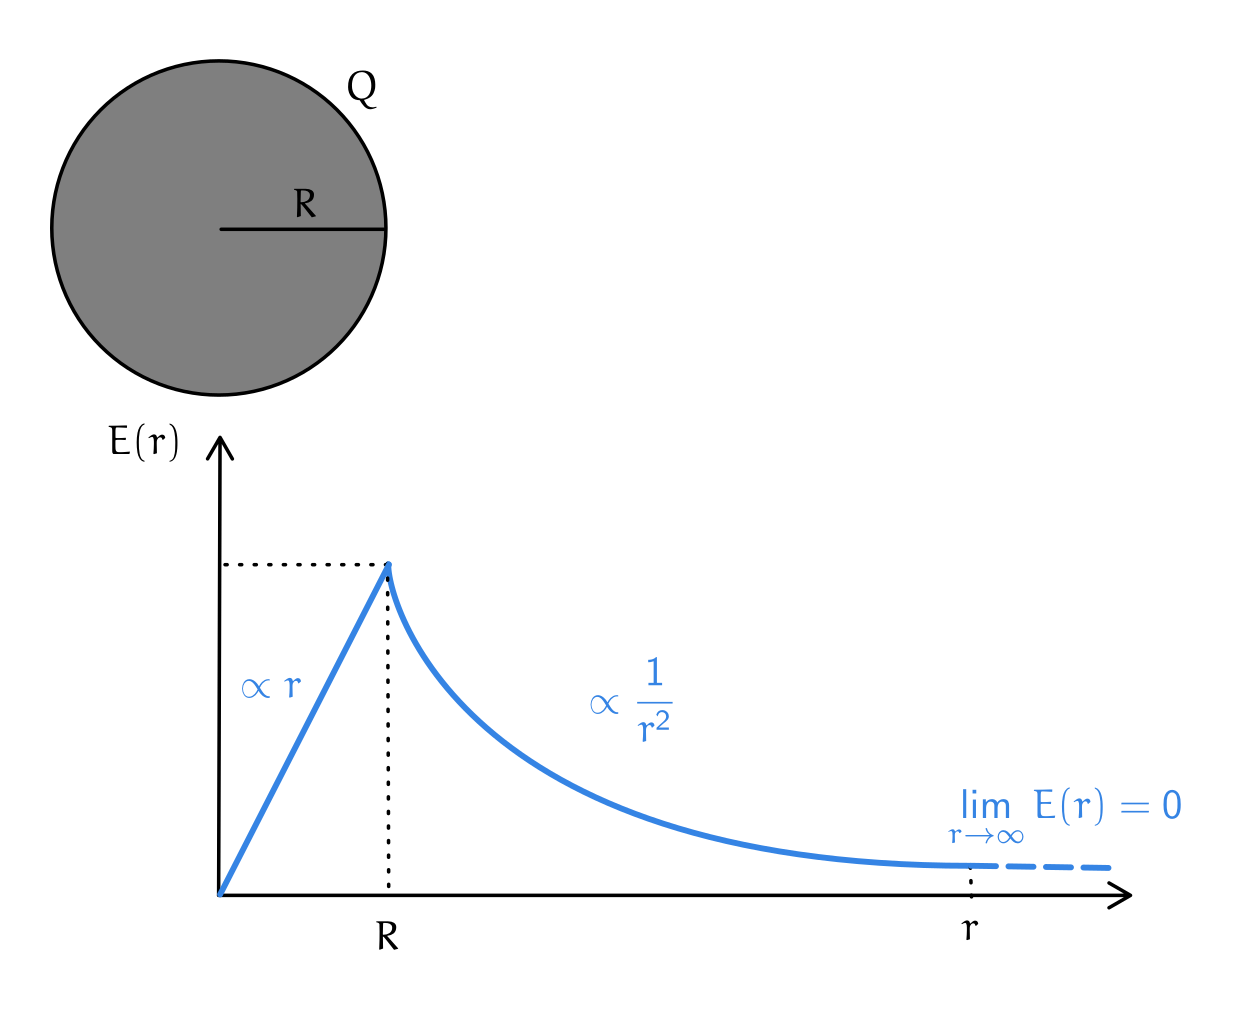
\includegraphics[width=0.9\textwidth]{grafico_volume_sferico}
  \end{figure}
\end{example}

\subsubsection{Simmetria cilindrica}
Le possibili simmetrie sono:
\begin{itemize}
  \item Filo indefinito con distribuzione di carica lineare \( \lambda \)
  \item Cilindro
    \begin{itemize}
      \item Con distribuzione di carica sulla superficie
      \item Con distribuzione di carica nel volume
    \end{itemize}
\end{itemize}
La caratteristica principale è la \textbf{simmetria attorno all'asse del sistema}.
La superficie di Gauss in cui il campo è costante è un cilindro di raggio \( r \) e
altezza \( h \).
\begin{example}
  Consideriamo una carica \( \lambda^+ \) distribuita su un filo indefinito:
  \begin{figure}[H]
    \centering
    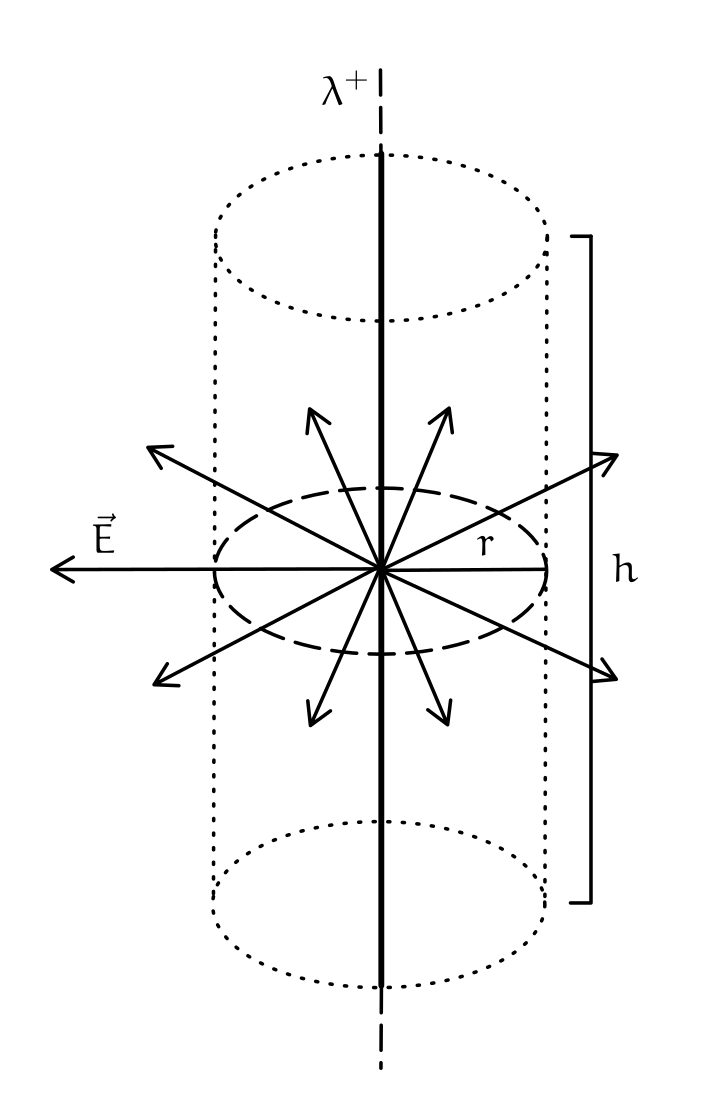
\includegraphics[width=0.5\textwidth]{carica_filo_indefinito}
    \caption{Carica distribuita su un filo indefinito}
  \end{figure}
  \noindent
  Il flusso del campo è il flusso delle basi (che essendo perpendicolari al campo radiale
  vale 0) più il flusso laterale:
  \[
    \Phi (\vec{E}) = \Phi_{\text{Basi}} + \Phi_{\text{Laterale}} = 0 + E \cdot 2 \pi r h =
    \frac{Q_{\text{Int}}}{\varepsilon_0} = \frac{\lambda h}{\varepsilon_0}
  \] 
  Quindi il campo è:
  \[
    E(r) = \frac{\lambda}{2 \pi \varepsilon_0 r}
  \] 
  Il grafico del campo elettrico è:
  \begin{figure}[H]
    \centering
    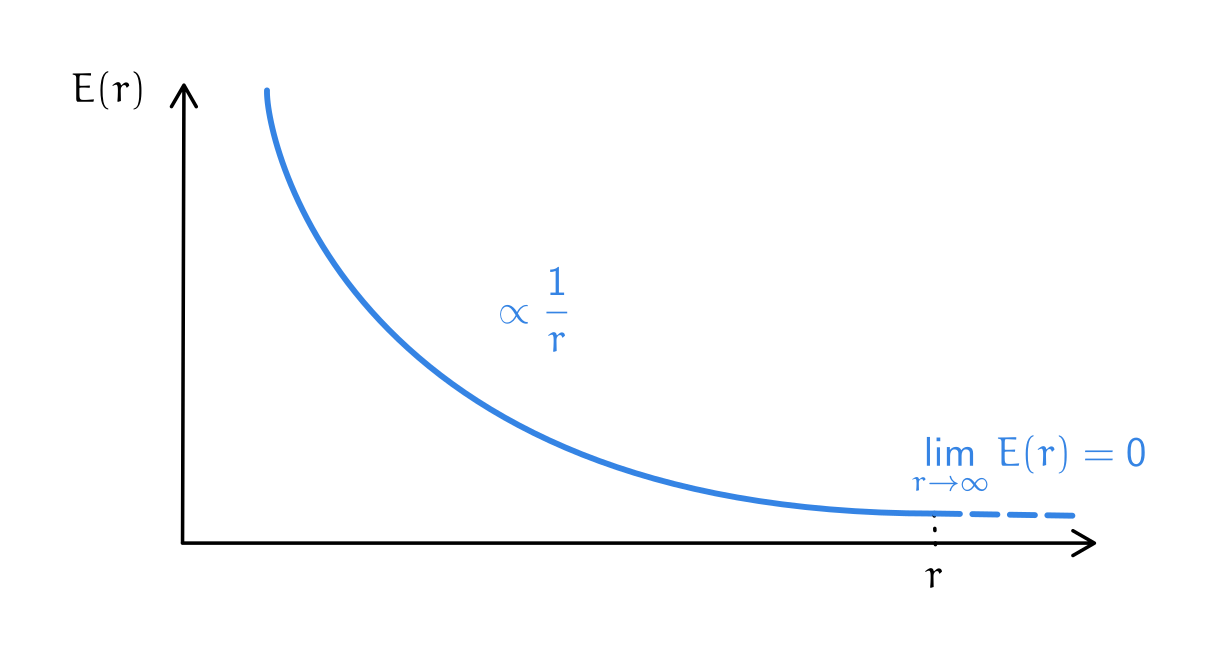
\includegraphics[width=0.9\textwidth]{grafico_filo_indefinito}
    \caption{Grafico del campo elettrico}
  \end{figure}
\end{example}
\begin{example}
  Consideriamo una carica \( \sigma^+ \) distribuita su un cilindro di raggio \( R \) e
  altezza \( h \):
  \begin{figure}[H]
    \centering
    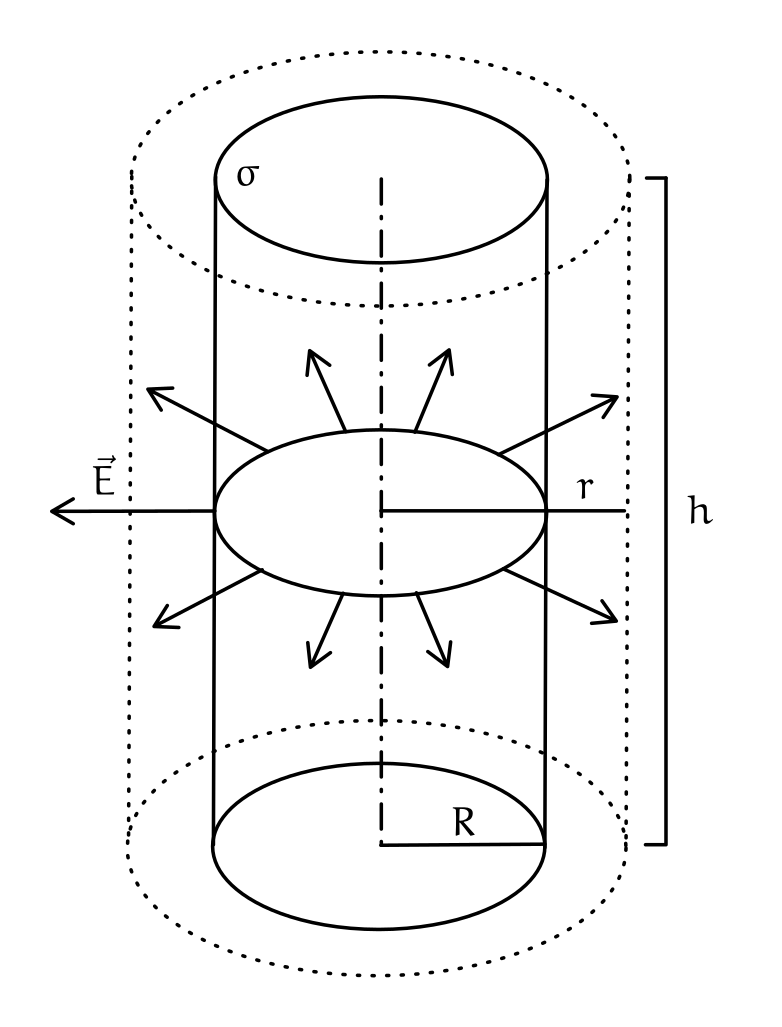
\includegraphics[width=0.5\textwidth]{carica_superficie_cilindrica}
    \caption{Carica distribuita su un cilindro di raggio \( R \) e altezza \( h \)}
  \end{figure}
  Il flusso del campo è lo stesso del caso precedente, ma con \( Q_{\text{Int}} \) diverso:
  \[
    Q_{\text{Int}} =
    \begin{cases}
      \sigma \cdot 2 \pi R h & \text{se } r \ge R\\
      0 & \text{se } r < R
    \end{cases}
  \] 
  Quindi il campo è:
  \[
    E(r) = \begin{cases}
      \frac{\sigma R}{\varepsilon_0 r} & \text{se } r \ge R\\
      0 & \text{se } r < R
    \end{cases}
  \]
  Il grafico del campo elettrico è:
  \begin{figure}[H]
    \centering
    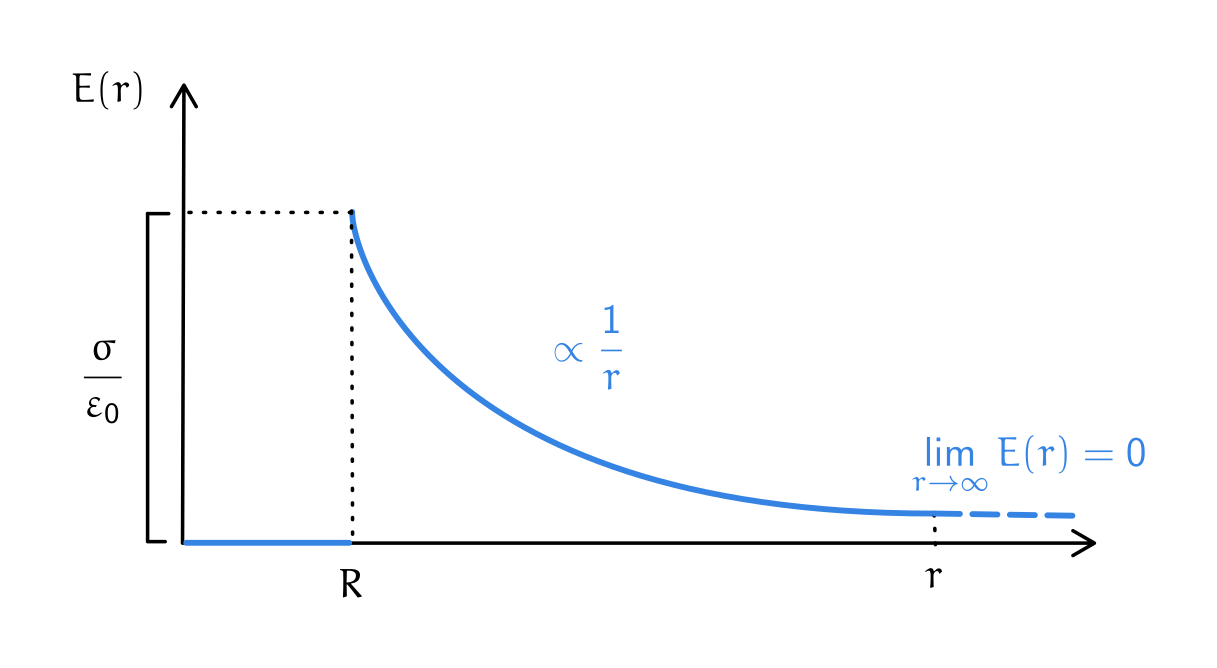
\includegraphics[width=0.9\textwidth]{grafico_superficie_cilindrica}
    \caption{Grafico del campo elettrico}
  \end{figure}
\end{example}

\subsubsection{Simmetria rispetto ad un piano indefinito}
Consideriamo un piano indefinito con una distribuzione di carica superficiale 
positiva \( \sigma^+ \; \left[ \frac{C}{m^2} \right] \). L'unico grado di libertà
è la distanza dal piano. L'elemento di campo è definito come:
\[
  d\vec{E} = \frac{dq}{4 \pi \varepsilon_0 r^2} \hat{r}
\] 
Se consideriamo un elemento di carica che agisce su un punto \( p \), allora siccome
il piano è indefinito ci sarà un elemento di carica simmetrico che genera un campo
con componente orizzontale uguale e opposto a quella dell'elemento precedente.
Di conseguenza il campo totale sarà perpendicolare al piano:
\begin{figure}[H]
  \centering
  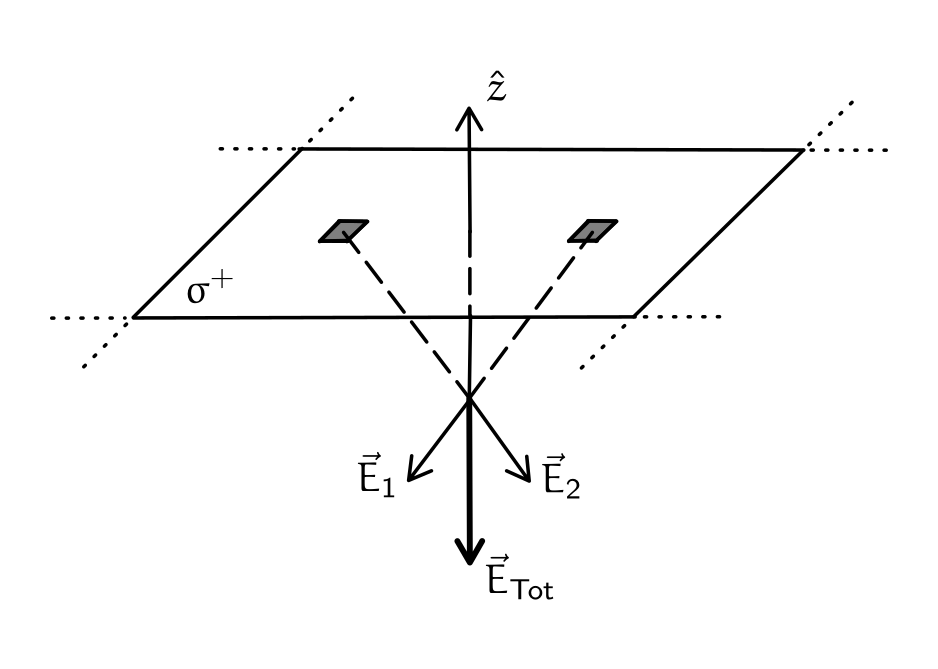
\includegraphics[width=0.7\textwidth]{carica_superficie_piano}
  \caption{Carica distribuita su un piano indefinito}
\end{figure}
\noindent
Il campo avrà questa forma:
\[
  \vec{E} = E(z) \hat{z}
\] 
La superficie di Gauss da considerare è un cilindro che si trova metà sopra e metà sotto
il piano:
\begin{figure}[H]
  \centering
  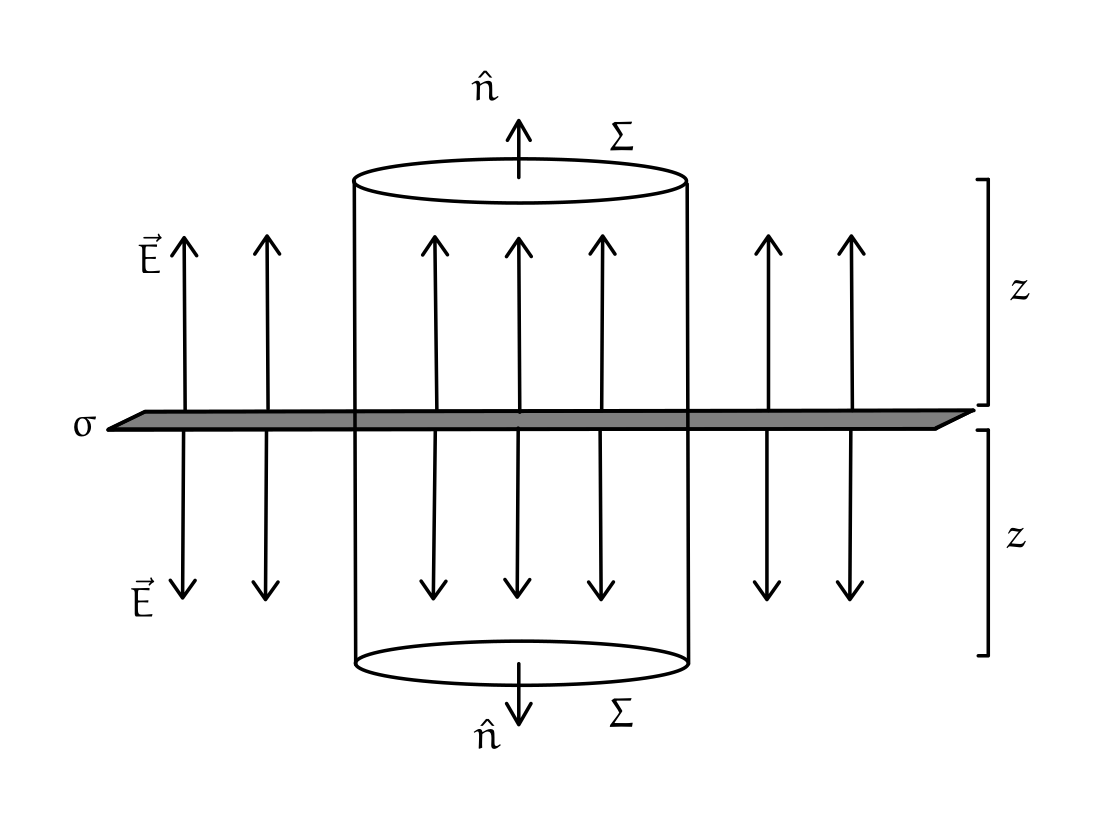
\includegraphics[width=0.8\textwidth]{superficie_gauss_piano}
  \caption{Superficie di Gauss per un piano indefinito}
\end{figure}
\noindent
Il flusso del sistema sarà il flusso delle basi più il flusso dei lati, ma il flusso
laterale sarà nullo:
\[
  \Phi = \Phi_{\text{Basi}} + \Phi_{\text{Laterale}} = 2 E(z) \cancel{\Sigma} + 0 
  = \frac{Q_{\text{Int}}}{\varepsilon_0} = \frac{\cancel{\Sigma} \sigma}{\varepsilon_0}
\] 
Quindi il campo è:
\[
  E = \frac{\sigma^\pm}{2 \varepsilon_0}
\] 
La particolarità di questo campo è che non dipende dalla distanza, quindi è un campo
costante.

\begin{example}
  Vogliamo analizzare il campo elettrico tra due piani indefiniti distanti \( h \) uno
  caricato positivamente e l'altro negativamente.
  \begin{figure}[H]
    \centering
    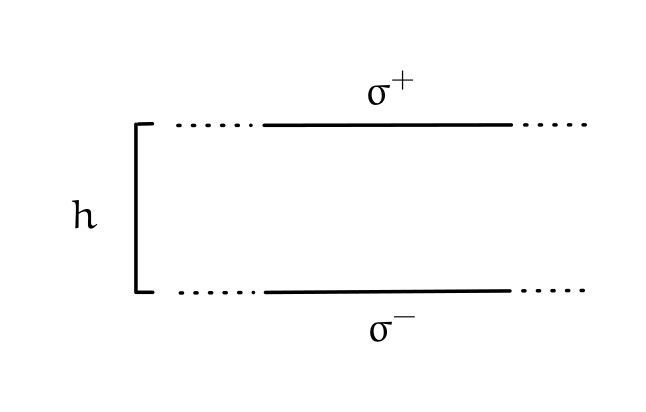
\includegraphics[width=0.5\textwidth]{carica_superficie_piano_positivo_negativo}
    \caption{Carica distribuita su due piani indefiniti}
  \end{figure}
  \noindent
  Il piano, per il principio di sovrapposizione, è uguale a:
  \[
    \sigma = \sigma ^+ + \sigma ^-
  \] 
  \begin{figure}[H]
    \centering
    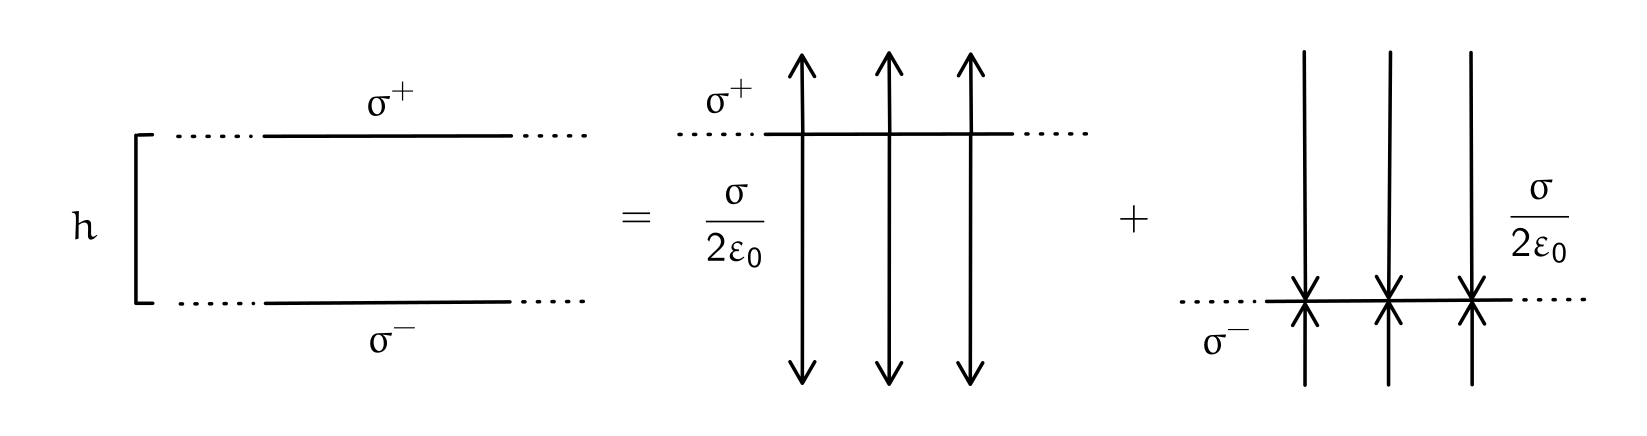
\includegraphics[width=1.\textwidth]{sovrapposizione_piano}
    \caption{Sovrapposizione di due piani}
  \end{figure}
  \noindent
  Dal teorema di Gauss abbiamo che il campo è costante e vale:
  \[
    \vec{E} = \frac{\sigma}{2 \varepsilon_0}
  \] 
  quindi:
  \begin{figure}[H]
    \centering
    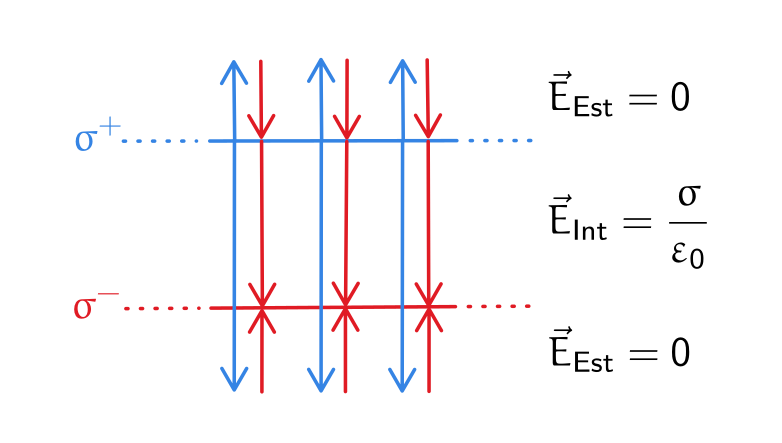
\includegraphics[width=0.7\textwidth]{sovrapposizione_piano_2}
    \caption{Risultato della sovrapposizione di due piani}
  \end{figure}
  \noindent
  Notiamo che all'esterno dei piani il campo è nullo, mentre al centro è la somma
  dei due campi con verso dal positivo al negativo.
  \[
    \vec{E} = \frac{\sigma}{2\varepsilon_0} + \frac{\sigma}{2\varepsilon_0} =
    \frac{\sigma}{\varepsilon_0}
  \] 
  Le linee di campo sono quindi:
  \begin{figure}[H]
    \centering
    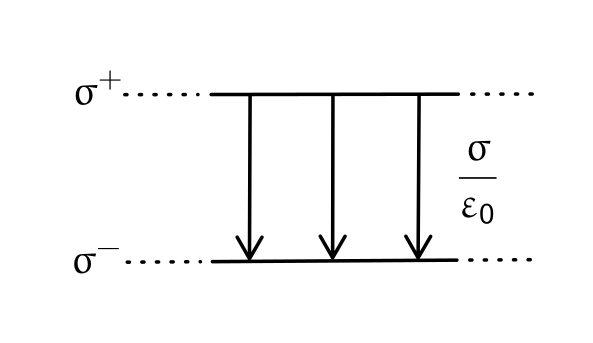
\includegraphics[width=0.5\textwidth]{linee_campo_piano}
    \caption{Linee di campo tra due piani}
  \end{figure}
\end{example}

\subsection{Elettrostatica nei conduttori}
Un materiale conduttore ha \textbf{le cariche libere di muoversi}. Se si avvicina un
campo elettrico e sulle cariche viene esercitata una forza. Per un momento ci sarà
del caos, ma poi le cariche si sposteranno fino a quando non si raggiunge l'equilibrio,
in quel momento si studia il comportamento delle cariche.

\subsubsection{Proprietà dei conduttori in equilibrio elettrostatico}
\begin{enumerate}
  \item \textbf{Prima proprietà}: Il campo totale interno in un conduttore è 0:
    \[
      E_{\text{Interno}} = 0
    \] 

    \vspace{1em}
    \noindent
    Consideriamo un conduttore immerso in un campo chiamato \textbf{campo esterno}.
    Le cariche sono libere di muoversi, quindi quelle positive andranno nella direzione
    del campo, mentre quelle negative andranno nella direzione opposta al campo.
    \begin{figure}[H]
      \centering
      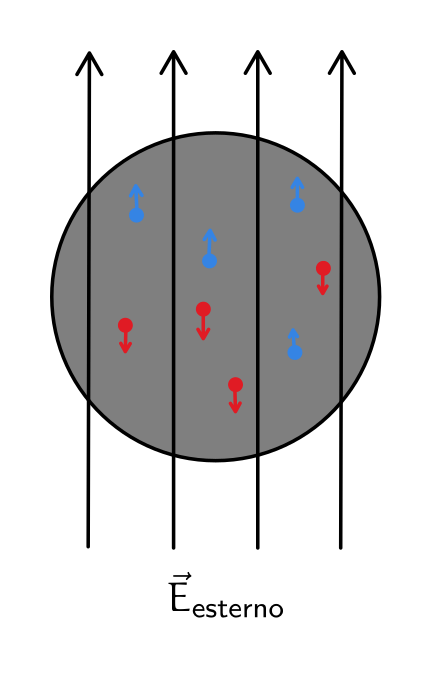
\includegraphics[width=0.4\textwidth]{conduttore_campo_esterno}
      \caption{Campo esterno in un conduttore}
    \end{figure}
    Si nota quindi una separazione di carica che creerà un \textbf{campo indotto}.
    \begin{figure}[H]
      \centering
      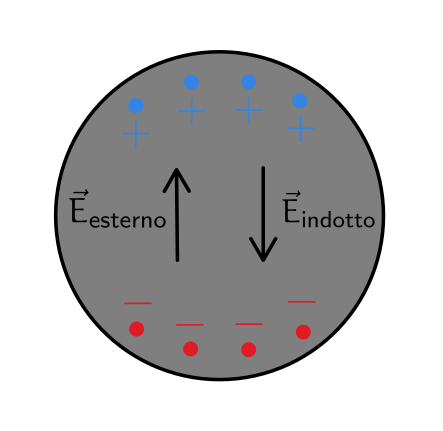
\includegraphics[width=0.4\textwidth]{conduttore_campo_indotto}
      \caption{Campo indotto in un conduttore}
    \end{figure}
    Vale il principio di sovrapposizione e quindi all'interno del conduttore si avrà
    la somma dei due campi:
    \[
      E_{\text{tot}} = E_{\text{est}} + E_{\text{ind}}
    \] 
    Ad un certo punto si raggiungerà l'equilibrio, quindi le cariche non si muovono più,
    di conseguenza il campo è nullo.

  \item \textbf{Seconda proprietà}: Siccome il campo è nullo, il potenziale è costante su
    tutto il conduttore:
    \[
      V - V_0 = - \int_{\vec{r}_0}^{\vec{r}} \cancel{\vec{E}} \cdot d\vec{l}
    \] 
    \[
      V = \text{costante}
    \] 

  \item \textbf{Terza proprietà}: Siccome il campo interno è nullo, la carica interna
    in un conduttore in equilibrio è 0 (dal teorema di Gauss) \( Q_{\text{Int}} = 0 \) :
    \[
      \oint_S \cancel{\vec{E}} \cdot d\vec{S} = \frac{Q_{\text{int}}}{\varepsilon_0} = 0 \to Q_{\text{int}} = 0
    \] 
    Quindi \textbf{le cariche si distribuiscono solo in superficie}

  \item \textbf{Quarta proprietà}: Il campo nella superficie di un conduttore è ortogonale 
    alla superficie e vale sempre:
    \[
      \vec{E}_{\text{sup}} = \frac{\sigma}{\varepsilon_0} \hat{n}
    \] 
    (Teorema di Coulomb)
\end{enumerate}
Notiamo quindi che il conduttore in equilibrio elettrostatico distorce il campo nel
seguente modo:
\begin{figure}[H]
  \centering
  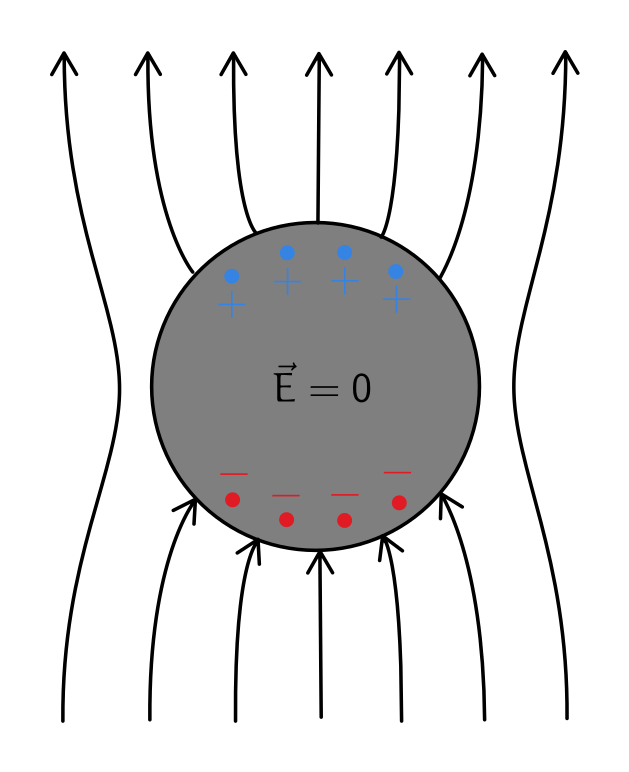
\includegraphics[width=0.5\textwidth]{conduttore_equilibrio}
  \caption{Campo in un conduttore in equilibrio}
\end{figure}

\subsubsection{Cavità in un conduttore}
La cavità non dipende dalla geometria del conduttore. Un esempio di un conduttore con
una cavità è il seguente (un guscio):
\begin{figure}[H]
  \centering
  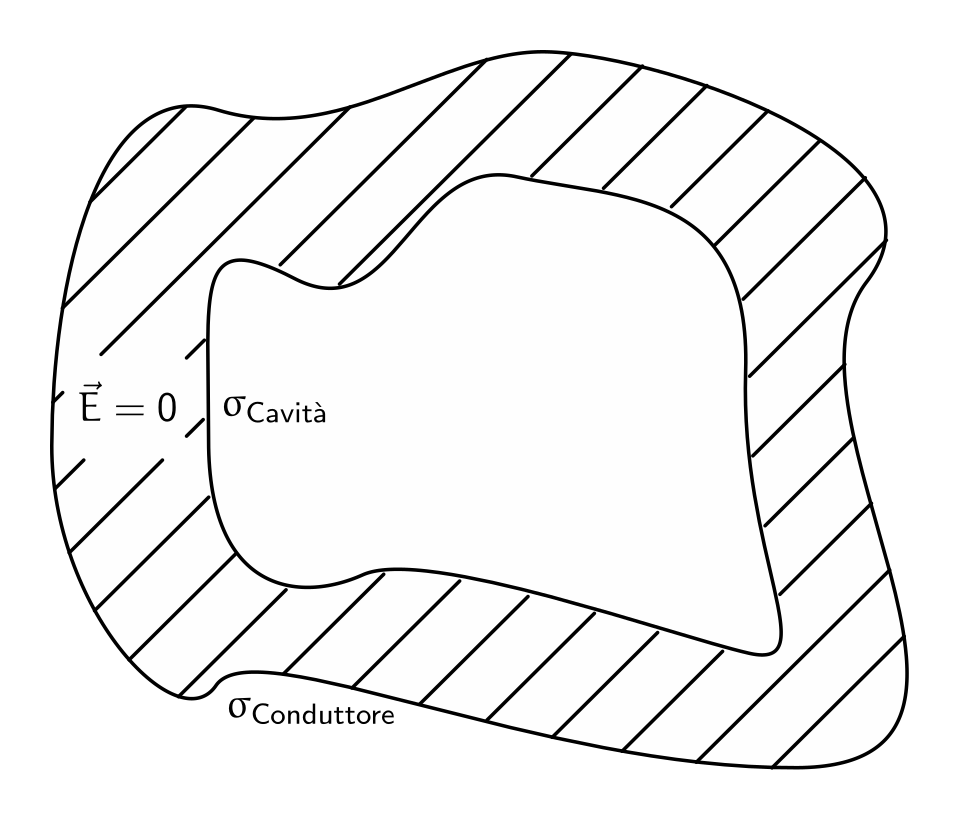
\includegraphics[width=0.6\textwidth]{conduttore_guscio}
  \caption{Conduttore con una cavità}
\end{figure}

\noindent
Carichiamo un conduttore con una cavità \textbf{vuota} con una carica \( Q \). Questa carica
si distribuirà sulla superficie del conduttore e ha le seguenti proprietà:
\begin{enumerate}
  \item La densità nella superficie della cavità è scarica:
    \[
      \sigma_{\text{Cavità}} = 0
    \] 
    quindi se si deposita una carica sul guscio, l'interno non può essere caricato
    
  \item Il campo all'interno della cavità è nullo:
    \[
      E_{\text{Cavità}} = 0
    \] 
    \textbf{Dimostrazione}: Per il teorema di Gauss posiziono una superficie di Gauss
    all'interno del conduttore, quindi:
    \begin{figure}[H]
      \centering
      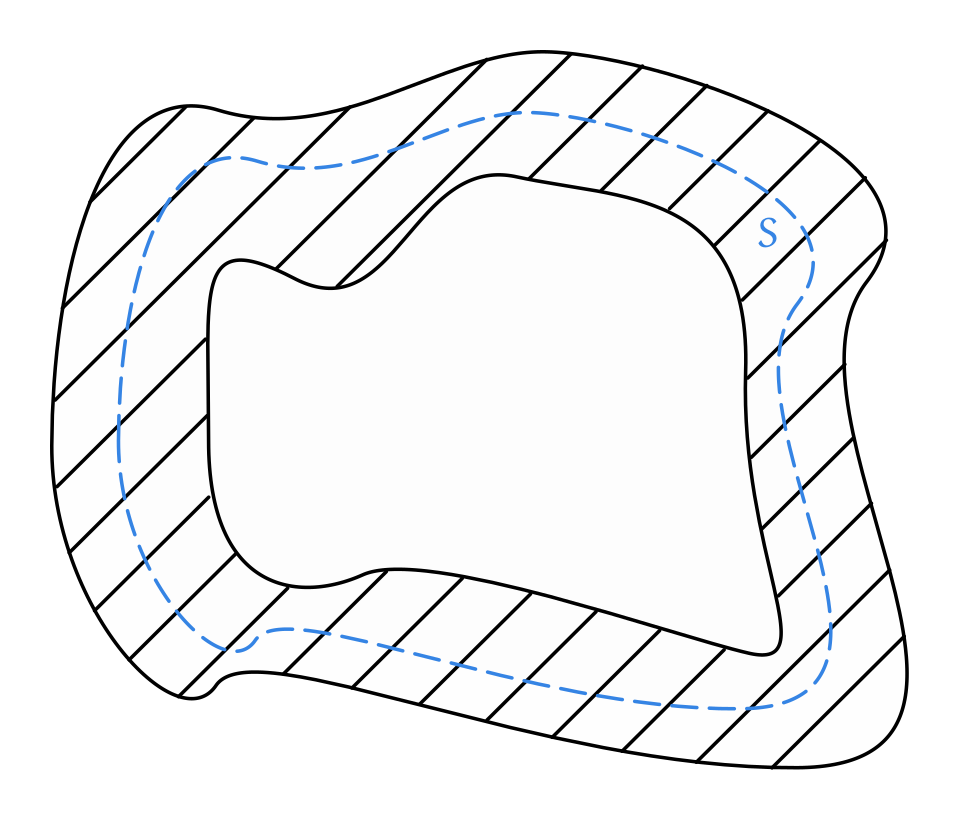
\includegraphics[width=0.6\textwidth]{superficie_gauss_conduttore_cavita}
      \caption{Superficie di Gauss in un conduttore con cavità}
    \end{figure}
    \[
      \oint_S \vec{E} \cdot d\vec{S} = \frac{Q_{\text{int \textbf{totale}}}}{\varepsilon_0}
    \] 
    Il campo vale 0 perchè la superficie di Gauss si trova all'interno del conduttore,
    quindi:
    \[
      \oint_S \vec{E} \cdot d\vec{S} = 0 \Rightarrow Q_{\text{Cavità}} = 0
    \] 
    La carica totale è nulla, però si potrebbe avere una situazione con una carica positiva
    e negativa che si annullano. Se per assurdo si avesse una separazione di carica,
    con carica totale nulla:
    \[
      q^+ + q^- = 0
    \] 
    allora ci sarebbe un campo interno:
    \begin{figure}[H]
      \centering
      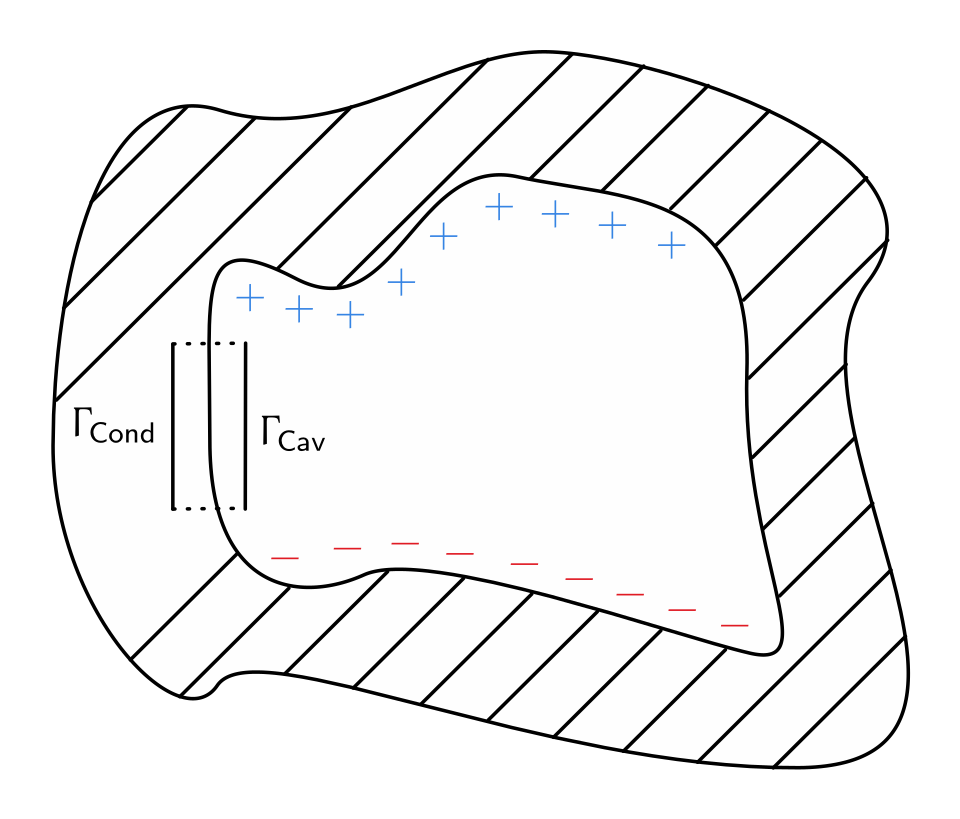
\includegraphics[width=0.6\textwidth]{dim_conduttore_cavita}
      \caption{Dimostrazione del campo nullo in un conduttore con cavità}
    \end{figure}
    per l'equazione di Maxwell sapppiamo che:
    \[
      \int_\Gamma E \cdot dl = \int_{\Gamma_{\text{Conduttore}}} E +
      \underbrace{\cancel{\int_{\Gamma_{\text{Cavità}}} E}}_{=0} \neq 0
    \] 
    E questo è assurdo, quindi il campo è nullo.
\end{enumerate}
Le linee di campo sono:
\begin{figure}[H]
  \centering
  \includegraphics[width=0.6\textwidth]{linee_campo_conduttore_cavita}
  \caption{Linee di campo in un conduttore con cavità}
\end{figure}
\noindent
Questa superficie con una cavità agisce come uno \textbf{schermo elettrostatico} (
o gabbia di Faraday) perchè il campo all'interno è nullo. 

\vspace{1em}
\noindent
Consideriamo ora un conduttore con una cavità \textbf{carica}, ciò vuol dire che
nella cavità è presente un conduttore carico e questa carica si distribuisce sulla
superficie:
\begin{figure}[H]
  \centering
  \includegraphics[width=0.6\textwidth]{conduttore_cavita_carica}
  \caption{Conduttore con una cavità carica}
\end{figure}
\noindent
Per Gauss posiziono una superficie all'interno del conduttore con la cavità, quindi:
\begin{figure}[H]
  \centering
  \includegraphics[width=0.6\textwidth]{superficie_gauss_conduttore_cavita_carica}
  \caption{Superficie di Gauss in un conduttore con cavità carica}
\end{figure}
\[
  \oint_S \underbrace{\vec{E}}_{=0} \cdot d\vec{S} = 0 = \frac{Q_{\text{int}}}{\varepsilon_0}
\] 
Visto che la carica deve essere 0, compare \textbf{per induzione} una carica uguale
ed opposta a quella della cavità:
\[
  Q_{\text{Indotta}} = - Q_{\text{Cavità}}
\]
Però la carica si conserva, quindi compare sempre per induzione una carica \( Q \)
sulla superficie esterna:
\begin{figure}[H]
  \centering
  \includegraphics[width=0.6\textwidth]{induzione_conduttore_cavita_carica}
  \caption{Induzione in un conduttore con cavità carica}
\end{figure}
\noindent
Le linee di campo sono:
\begin{figure}[H]
  \centering
  \includegraphics[width=0.6\textwidth]{linee_campo_conduttore_cavita_carica}
  \caption{Linee di campo in un conduttore con cavità carica}
\end{figure}
\noindent
Se viene aggiunta una carica all'esterno il sistema \textbf{nella cavità} non cambia
perchè la superficie agisce come uno schermo. All'esterno invece le cariche si sommano.

\begin{example}
  Consideriamo il seguente sistema:
  \begin{figure}[H]
    \centering
    \includegraphics[width=0.5\textwidth]{conduttore_cavita_sferica_carica}
    \caption{Conduttore con cavità sferica carica}
  \end{figure}
  \noindent
  Se si mette al contatto il conduttore interno con il conduttore esterno si ottiene il
  sistema del conduttore con una cavità perchè i due conduttori agiscono come se fossero
  uno solo:
  \begin{figure}[H]
    \centering
    \includegraphics[width=0.5\textwidth]{conduttore_cavita_sferica_carica_2}
    \caption{Trasformazione del condensatore in un conduttore con cavità carica}
  \end{figure}
\end{example}

\subsection{Capacità elettrostatica}
Un carica \( \{dq\}  \) genera un campo
\[
  d\vec{E} = \frac{\{dq\}}{4 \pi \varepsilon _0} \frac{\hat{r}}{r^2} \quad \left[ \frac{V}{m} \right]
\]
e un potenziale
\[
  dV = \frac{\{dq\}}{4 \pi \varepsilon_0 r} \quad \left[ V \right]
\] 
Osserviamo che c'è una linearità tra la carica e il potenziale, quindi \( V \) è
proporzionale a \( Q \) e il coefficiente di proporzionalità è la \textbf{capacità}.

\subsubsection{Conduttore isolato}
Consideriamo un qualsiasi conduttore isolato con una carica \( Q \) e un potenziale
\( V \) costante.

\begin{definition}
  Si definisce \textbf{capacità elettrostatica} \( C \) di un conduttore isolato la
  quantità di carica \( Q \) tarsferita al conduttore da un potenziale \( V \)
  \[
    C = \frac{Q}{V} \quad \left[ F \right] \text{ (Farad)}
  \]
  La capacità dipende solo dalla geometria e dal materiale.
\end{definition}

\subsubsection{Conduttore non isolato}
Consideriamo due conduttori, uno con carica \( Q \) e uno con carica \( -Q \) in
\textbf{induzione completa}, cioè tutte le linee di campo del primo oggetto vanno nel
secondo oggetto. Per avere ciò bisogna eliminare ogni interazione con l'esterno e l'unica
opzione è inserire il primo oggetto nella cavità del secondo.
\begin{figure}[H]
  \centering
  \includegraphics[width=0.5\textwidth]{conduttore_isolato}
  \caption{Isolamento di un conduttore}
\end{figure}
\noindent
Un \textbf{Condensatore} è un sistema di due conduttori in induzione completa. In
un condensatore i due conduttori si dicono \textbf{armature} o \textbf{lastre}.

\vspace{1em}
\noindent
Nella pratica si distinguono 3 casi (in questo corso):
\begin{enumerate}
  \item \textbf{Condensatore sferico}: Si hanno due sfere, una nella concavità 
    dell'altra
    \begin{figure}[H]
      \centering
      \includegraphics[width=0.5\textwidth]{condensatore_sferico}
      \caption{Condensatore sferico}
    \end{figure}

  \item \textbf{Condensatore cilindrico}: È una struttura tubolare, in cui
    se il raggio è molto minore della lunghezza del tubo allora si può \textbf{approssimare}
    come un induzione completa:
    \begin{figure}[H]
      \centering
      \includegraphics[width=0.5\textwidth]{condensatore_cilindrico}
      \caption{Condensatore cilindrico}
    \end{figure}

  \item \textbf{Condensatore piano}: È formato da due lastre piane parallele
    separate da una distanza \( h \) con una certa area \( A \). Anche in questo
    caso se le lastre sono molto grandi rispetto alla distanza si può approssimare
    come un induzione completa.
    \begin{figure}[H]
      \centering
      \includegraphics[width=0.7\textwidth]{condensatore_piano}
      \caption{Condensatore piano}
    \end{figure}
\end{enumerate}

\subsubsection{Capacità nei condensatori}
Consideriamo un condensatore:
\begin{figure}[H]
  \centering
  \includegraphics[width=0.5\textwidth]{potenziale_condensatore_sferico}
  \caption{Condensatore sferico}
\end{figure}
\noindent
La capacità è:
\[
  C = \frac{Q}{\Delta V} \quad \text{(presa positiva)}
\] 

\begin{example}
  Calcoliamo la capacità del condensatore piano nel vuoto, indicato con il seguente simbolo:
  \begin{figure}[H]
    \centering
    \begin{circuitikz}
      \draw (0,0) to[C] (2,0);
    \end{circuitikz}
    \caption{Condensatore piano}
  \end{figure}
  \noindent
  Consideriamo un piano con carica positiva e uno con carica negativa e area \( A \):
  \begin{figure}[H]
    \centering
    \includegraphics[width=0.7\textwidth]{potenziale_condensatore_piano}
    \caption{Potenziale di un condensatore piano}
  \end{figure}
  \noindent
  Il campo è solo all'interno e vale:
  \[
    E = \frac{\sigma}{\varepsilon_0}
  \] 
  La capacità è:
  \[
    C = \frac{Q}{V^+ - V^-}
  \] 
  Ora bisogna calcolare la differenza di potenziale tra le due lastre ricordando la
  definizione di potenziale:
  \[
    V_2 - V_1 = -\int_1^2 \vec{E} \cdot d\vec{l}
  \] 
  quindi
  (Il campo è negatico perchè la sua direzione è opposta a quella del potenziale):
  \[
    V^+ - V^- = - \int_-^+ \left( - \frac{\sigma}{\varepsilon_0} \right) dx 
    = \frac{\sigma }{\varepsilon _0} h \quad \left[ V \right]
  \] 
  Di conseguenza la capacità è:
  \[
    C = \frac{Q}{\frac{\sigma}{\varepsilon_0} h} = \frac{\sigma A}{\frac{\sigma}{\varepsilon_0} h}
    = \frac{\varepsilon_0 A}{h} \quad \left[ F \right]
  \]
\end{example}

\subsection{Calcolo del campo potenziale}
\subsubsection{Simmetria sferica}
Il campo di una superficie sferica è:
\[
  \vec{E} =
  \begin{cases}
    \frac{Q}{4 \pi \varepsilon_0 r^2} \hat{r} & r \ge R\\
    0 & r < R
  \end{cases}
\] 
La definizione di potenziale è:
\[
  V(r) - V_{\text{Riferimento}} = - \int_{\gamma }\vec{E} \cdot d\vec{l}
  = -\int_{\vec{r_0}}^{\vec{r}} \vec{E}(r) \, dr
\] 
dove \( V_{\text{Riferimento}} = V(rif) \to V(\infty) = 0 \). Il potenziale di reiferimento
\textbf{può} essere preso all'infinito soltanto per sistemi in cui \textbf{non} ci sono
cariche all'infinito.

Quindi il calcolo del potenziale diventa:
\[
  V(r) - \underset{=0}{\cancel{V_{\text{Riferimento}}}}
  = - \int_{\infty}^{r} \frac{Q}{4 \pi \varepsilon_0 r^2} \, dr
  = - \left.\left( \frac{-Q}{4 \pi \varepsilon_0 r} \right)\right|_{\infty}^{r}
    = \frac{Q}{4 \pi \varepsilon_0 r} \quad \left[ V \right]
\] 
(solo per \( r > R \)). Il grafico è:
\begin{figure}[H]
  \centering
  \includegraphics[width=0.9\textwidth]{grafico_potenziale}
  \caption{Grafico del potenziale}
\end{figure}

\begin{definition}
  Il potenziale si calcola come:
  \[
    V(r) =
    \begin{cases}
      \frac{Q}{4 \pi \varepsilon_0 r} & r \ge R\\
      \text{Costante} & r < R
    \end{cases}
  \] 
\end{definition}

\vspace{1em}
\noindent
Con il potenziale si può calcolare la capacita come:
\[
  C = \frac{Q}{V_{\text{Sup}}} = \frac{Q}{\frac{Q}{4 \pi \varepsilon_0 R}}
  = 4 \pi \varepsilon_0 R \quad \left[ F \right]
\] 

\begin{example}[Potenziale di un condensatore sferico]
  Consideriamo un condensatore sferico con carica \( Q \) in cui il raggio del conduttore
  sferico interno è \( R_1 \) e i raggi del conduttore sferico sono \( R_2 \) e \( R_3 \).
  Il campo è:
  \[
    \vec{E} = \frac{Q}{4 \pi \varepsilon_0 r^2} \hat{r} \quad R_1 < r < R_2
  \] 
  Il campo è nullo nei seguenti casi:
  \[
    \vec{E} = 0 \to \begin{cases}
      r < R_1\\
      R_2 < r < R_3
    \end{cases}
  \] 
  quindi all'interno del conduttore.

  Il potenziale sarà:
  \[
    V(r) = \frac{Q}{4 \pi \varepsilon_0 r} \quad \left[ V \right] \quad \text{Nella cavità}
  \] 
  All'interno dei conduttori il potenziale vale:
  \[
    \begin{aligned}
      V(R_1) &= \frac{Q}{4 \pi \varepsilon_0 R_1}\\
      V(R_2) &= \frac{Q}{4 \pi \varepsilon_0 R_2}
    \end{aligned}
  \] 
  La capacità è:
  \[
    C = \frac{Q}{\Delta V} = \frac{Q}{V(R_2) - V(R_1)}
    = \frac{Q}{\frac{Q}{4 \pi \varepsilon_0 \left( \frac{1}{R_1} - \frac{1}{R_2} \right)}}
    = 4 \pi \varepsilon_0 \frac{R_1 R_2}{R_2 - R_1} \quad \left[ F \right]
  \] 
\end{example}
\begin{example}[Potenziale in un filo indefinito]
  Consideriamo un filo indefinito conduttore con carica \( \lambda \). Il campo
  è:
  \[
    \vec{E} = \frac{\lambda}{2 \pi \varepsilon_0 r}
  \] 
  Il potenziale è calcolato come:
  \[
    V(r) - \underset{=0}{\cancel{V(rif)}} = - \int_{rif}^r \frac{\lambda}{2 \pi \varepsilon_0 r} \, dr
    = - \frac{\lambda}{2 \pi \varepsilon_0} \left( \ln(r) - \ln(rif) \right) 
  \] 
  Vogliamo che il punto di riferimento renda nullo il potenziale, quindi:
  \[
    V(rif) = 0
  \] 
  quindi il punto di riferimento è un punto qualunque
  \[
    rif \neq \infty
  \] 
  Il grafico del potenziale è:
  \begin{figure}[H]
    \centering
    \includegraphics[width=0.9\textwidth]{grafico_potenziale_filo}
    \caption{Grafico del potenziale}
  \end{figure}
\end{example}

\subsection{Elettrostatica nei dielettrici}
\subsubsection{Polarizzazione}
I dielettrici hanno cariche vincolate.

\begin{enumerate}
  \item 
    Consideriamo un atomo neutro,
    applichiamo un campo e osserviamo che le cariche negative si separano in direzione
    del campo:
    \begin{figure}[H]
      \centering
      \includegraphics[width=0.8\textwidth]{dipolo_atomo}
      \caption{Atomo in un campo}
    \end{figure}
    \noindent
    Questo sistema si può modellare nel seguente modo:
    \begin{figure}[H]
      \centering
      \includegraphics[width=0.6\textwidth]{dipolo}
      \caption{Dipolo elettrico}
    \end{figure}
    \noindent
    Due cariche opposte \( q \) e \( -q \) rigidamente separate da una distanza \( \vec{d} \)
    formano un \textbf{dipolo elettrico} (che produce un campo). Questo oggetto è caratterizzato dal
    \textbf{momento di dipolo elettrostatico}:
    \[
      \vec{p} = q \vec{d}
    \] 
    Quindi il materiale si \textbf{polarizza}, cioè si è creata una separazione di carica
    rigidamente separata.

  \item 
    Alcune molecole sono già polarizzate e si chiamano \textbf{molecole polari}, ad esempio
    l'acqua:
    \begin{figure}[H]
      \centering
      \includegraphics[width=0.5\textwidth]{molecola_acqua}
      \caption{Molecola di acqua}
    \end{figure}

  \item 
    Quando si ha un insieme di molecole polarizzate casualmente si ha un materiale
    globalmente neutro:
    \begin{figure}[H]
      \centering
      \includegraphics[width=0.7\textwidth]{molecole_polarizzate_casualmente}
      \[
        \vec{p}_{\text{tot}} = 0
      \] 
      \caption{Molecole polarizzate casualmente}
    \end{figure}
    \noindent
    Se si applica un campo esterno si ha una polarizzazione del materiale i momenti
    di dipolo si allineano per rotazione e il materiale si \textbf{polarizza per
    orientamento}:
    \begin{figure}[H]
      \centering
      \includegraphics[width=0.7\textwidth]{polarizzazione_orientamento}
      \caption{Polarizzazione per orientamento}
    \end{figure}
\end{enumerate}
\vspace{1em}
\noindent
Si introduce un oggetto chiamato \textbf{campo di polarizzazione} che misura
la polarizzazione del materiale per unità di volume:
\[
  \mathbb{P}(r) = \text{Momento di dipolo per unità di volume}
\] 

\begin{exercise}[Esperimento condensatore con dielettrico]
  Consideriamo un condensatore piano e carichiamo le lastre (collegandole ad una batteria)
  \begin{figure}[H]
    \centering
    \includegraphics[width=0.5\textwidth]{circuito_condensatore_1}
    \caption{Circuito con un condensatore}
  \end{figure}
  \noindent
  Sappiamo che nel vuoto:
  \begin{itemize}
    \item \( Q = C_0 V_0 \) 
    \item \( C_0 = \frac{\varepsilon_0 A}{h} \)
    \item \( E_0 = \frac{\sigma_0}{\varepsilon_0} \) 
  \end{itemize}
  Poi stacchiamo il circuito, e quindi il sistema diventa isolato, cioè la carica si
  conserva \( Q_{\text{tot}} = \text{Costante} \):
  \begin{figure}[H]
    \centering
    \includegraphics[width=0.5\textwidth]{circuito_condensatore_2}
    \caption{Circuito con un condensatore isolato}
  \end{figure}
  \noindent
  Riempiamo il condensatore con materiale dielettrico. Osserviamo che il potenziale
  nel dielettrico scala di un fattore \( k \) (diminuisce):
  \begin{figure}[H]
    \centering
    \includegraphics[width=0.5\textwidth]{circuito_condensatore_3}
    \caption{Circuito con un condensatore e dielettrico}
  \end{figure}
  \[
    V_k = \frac{V_0}{k} < V_0
  \] 
  Quindi la differenza di potenziale tra le armature diminuisce, quindi
  la capacità aumenta di \( k \) :
  \[
    C_k = \frac{Q}{V} = \frac{Q}{\frac{V_0}{k}} = k C_0
  \]
  La \( k \) è tipica del materiale dielettrico e si chiama \textbf{costante dielettrica}.
  (Il vuoto è un dielettrico con \( k_{\text{vuoto}} = 1 \)).

  \vspace{1em}
  \noindent
  Se il potenziale diminuisce, il campo diminuisce:
  \[
    V_k < V_0 \Rightarrow E_k = \frac{E_0}{k} < E_0
  \] 
  Quindi si è formato un campo opposto indotto \( E_{\text{Indotto}} \) che si somma
  al campo \( E_0 \) e quindi il campo totale è:
  \[
    E_{k} = E_0 + E_{\text{Indotto}}
  \]
  All'interno del dielettrico si è formata una carica di polarizzazione opposta:
  \begin{figure}[H]
    \centering
    \includegraphics[width=0.8\textwidth]{circuito_condensatore_4}
    \caption{Cariche di polarizzazione}
  \end{figure}
\end{exercise}

\subsubsection{Equazioni dell'elettrostatica nei dielettrici}
Consideriamo un condensatore piano:
\begin{figure}[H]
  \centering
  \includegraphics[width=0.6\textwidth]{condensatore_piano_dielettrico}
  \caption{Condensatore piano con dielettrico}
\end{figure}
\noindent
Con il teorema di Gauss prendiamo un cilindro di Gauss che ha una base nell'armatura
e una nel dielettrico:
\begin{figure}[H]
  \centering
  \includegraphics[width=0.8\textwidth]{gauss_condensatore_piano_dielettrico}
  \caption{Superficie di Gauss in un condensatore piano con dielettrico}
\end{figure}
\noindent
Applichiamo Gauss all'interno del cilindro calcolando il flusso:
\begin{figure}[H]
  \centering
  \includegraphics[width=0.4\textwidth]{gauss_condensatore_piano_dielettrico_2}
  \caption{Flusso del campo elettrico in un condensatore piano con dielettrico}
\end{figure}
\[
  \begin{aligned}
    \oint_S \vec{E} \cdot \hat{n} dS &= \vec{E}_{\underset{\text{Conduttore}}{\text{Tot}}}
    \Sigma + \vec{E}_{\underset{\text{Dielettrico}}{\text{Tot}}} \Sigma \\
    &= 0 + E_{\underset{\text{Dielettrico}}{\text{Tot}}} \Sigma\\
    &= \frac{Q_{\text{int}}}{\varepsilon_0}\\
    &= \frac{\sigma _0 \cancel{\Sigma} }{\varepsilon _0}
    - \frac{\sigma _{\text{pol}} \cancel{\Sigma} }{\varepsilon _0} \\
  \end{aligned}
\] 
Quindi il campo totale è:
\[
  E_k = \frac{\sigma _0}{\varepsilon _0} - \frac{\sigma _{\text{pol}}}{\varepsilon _0}
\] 
Di conseguenza un dipolo induce una carica opposta di polarizzazione:
\[
  |\sigma_{\text{Pol}}| = |\sigma_0| \frac{k-1}{k}
\] 

\vspace{1em}
\noindent
Consideriamo un volume unitario \( Vol_1 \) con superfici unitarie \( \Sigma_1 \).
Il numero di dipoli all'interno del volume per il momento del dipolo è la
polarizzazione \( \mathbb{P} \):
\[
  \frac{\text{\#atomi}}{Vol} \cdot \underbrace{\vec{p}}_{q\vec{d}} = \mathbb{P}
\] 
Quindi abbiamo che le cariche di polarizzazione sono equivalenti alla polarizzazione:
\[
  |\sigma_{\text{Pol}}| = \mathbb{P}
\] 
In termini generali:
\[
  \sigma_{\text{Pol}} = \mathbb{P} \cdot \hat{n}
\] 
Le cariche di polarizzazione si formano sulle superfici del dielettrico.

\subsubsection{Teorema di Gauss}
Prendiamo in considerazione un condensatore piano riempito con un dielettrico, abbiamo
che il flusso del campo elettrico è:
\[
  \begin{aligned}
    \oint \vec{E} &= \underbrace{\frac{\sigma_0}{\varepsilon_0} \Sigma}_{Q} - 
    \underbrace{\frac{\sigma_{\text{Pol}}}{\varepsilon_0} \Sigma}_{\text{Flusso di } \vec{\mathbb{P}}}
  \end{aligned}
\] 
Quindi abbiamo il teorema di Gauss:
\[
  \oint \left( \varepsilon_0 \vec{E} - \vec{\mathbb{P}} \right) \cdot \hat{n} dS = Q_{\text{Libere}}
\] 
Il campo \( \left( \varepsilon_0 \vec{E} - \vec{\mathbb{P}} \right) \) si chiama 
\textbf{spostamento dielettrico} o \textbf{induzione} \( \vec{D} \).

\begin{itemize}
  \item Nel vuoto:
    \[
      \oint_S \vec{E} \cdot \hat{n} dS = \frac{Q_{\text{Tot}}}{\varepsilon_0}
    \] 
    dove le cariche totali sono:
    \[
      Q_{\text{Tot}} = Q_{\text{Libere}} + Q_{\text{Polarizzazione}}
    \] 

  \item Nel dielettrico:
    \[
      \oint_S \vec{D} \cdot \hat{n} dS = Q_{\text{Libere}}
    \] 
\end{itemize}

\subsection{Energia elettrostatica}
Se un campo agisce su una carica essa sentirà una forza, quindi si può calcolare un'energia
\begin{figure}[H]
  \centering
  \includegraphics[width=0.6\textwidth]{energia_elettrostatica}
  \[
    \frac{1}{2} mv^2 + qV = \text{Costante}
  \] 
  \caption{Energia elettrostatica}
\end{figure}
\begin{definition}
  L'energia di un sistema è il lavoro esterno per costruire il sistema

  \begin{itemize}
    \item In un sistema discreto ci saranno \( N \) cariche discrete \( q_i \) 
    \item In un sistema continuo ci sarà una carica continua \( \rho \) 
  \end{itemize}
\end{definition}

\subsubsection{Energia di N cariche discrete}
Si calcola il lavoro esterno per portare la prima carica \( q_1 \) dall'infinito
\[
  L_1 = 0
\] 
Il lavoro è nullo perchè è la prima carica.

La seconda carica \( q_2 \)  trova un campo, quindi il suo lavoro è
\[
  L_2 = q_2 \Delta V_1
\] 
Il potenziale è quello del campo della prima carica. Sappiamo che \( V_\infty = 0 \),
quindi:
\[
  L_2 = q_2 \Delta V_1 = q_2 V_1(r_2) = \frac{q_2 q_1}{4 \pi \varepsilon_0 r_{12}}
\] 
Per l'n-esima carica \( q_n \) il lavoro è:
\[
  L_n = q_n V_1(r_n) + q_n V_2(r_n) + \ldots + q_n V_{n-1}(r_n)
\]
\begin{figure}[H]
  \centering
  \includegraphics[width=0.8\textwidth]{energia_cariche_discrete}
  \caption{Energia di un sistema discreto}
\end{figure}

\vspace{1em}
\noindent
L'energia del sistema è quindi:
\[
  \begin{aligned}
    U_{el} &= \frac{1}{2} \sum_{i=1}^N q_i V_i\\
           &= \frac{1}{2} \sum_i \sum_{j \neq i} \frac{q_i q_j}{r \pi \varepsilon_0 r_{ij}}
  \quad [J]
  \end{aligned}
\] 

\subsubsection{Energia in un sistema continuo}
Il procedimento è lo stesso del sistema discreto, solo che le sommatorie diventeranno
integrali e le cariche diventeranno densità di carica:
\[
  \sum \to \int \quad q_i \to \rho d\tau = dq
\] 
Quindi:
\[
  U_{el} = \frac{1}{2} \int_{\text{vol}} \int_{\text{vol}}
  \frac{
    \rho(r_1) \rho(r_2) \, d\tau_1 d\tau_2
  }{
    4 \pi \varepsilon_0 r_{12}
  }
  \quad [J]
\] 

\subsubsection{Energia con N conduttori}
Applichiamo la formula dell'energia in un sistema continuo
\[
  \begin{aligned}
    U_{el} &= \frac{1}{2} \int_{\text{vol}} \rho V \, d\tau\\
           &= \frac{1}{2} \int_{\text{sup}} \sigma V_0 \, dS \\
           &= \frac{1}{2} V_0 \underbrace{\int_{\text{sup}} \sigma \, dS}_{Q_0} \\
           &= \frac{1}{2} V_0 Q_0  \quad [J]\
  \end{aligned}
\] 
Quindi l'energia di un conduttore è:
\[
  \begin{aligned}
    U_{\text{cond}} &= \frac{1}{2} Q V\\
    &= \frac{1}{2} \frac{Q^2}{C} \\
    &= \frac{1}{2} C V^2 \
  \end{aligned}
\] 

\vspace{1em}
\noindent
Se consideriamo \( N \) conduttori l'energia è la somma delle energie dei singoli
conduttori:
\[
  U_{\text{Tot}} = \sum_{i=1}^N U_i = \frac{1}{2} \sum_{i=1}^N Q_i V_i
\] 

\vspace{1em}
\noindent
Un condensatore è semplicemente un sistema di due conduttori in induzione completa, quindi
\[
  \begin{aligned}
    U_{el} &= \frac{1}{2} (Q_1 V_1 + Q_2 + V_2)\\
    &= \frac{1}{2} Q \Delta V \\
    &= \frac{1}{2} C \Delta V^2 \\
    &= \frac{1}{2} \frac{Q^2}{C} \
  \end{aligned}
\] 

\subsubsection{Processo di carica del condensatore}
Un condensatore diventa tale solo dopo che viene caricato, quidi all'inizio è
semplicemente un'insieme di conduttori:
\begin{figure}[H]
  \centering
  \includegraphics[width=0.3\textwidth]{condensatore_piano_non_carico}
  \caption{Condensatore non carico}
\end{figure}
\noindent
Per caricare il condensatore si prende una carica positiva \( q^+ \) e si sposta
da un armatura all'altra:
\begin{figure}[H]
  \centering
  \includegraphics[width=0.4\textwidth]{condensatore_piano_carico}
  \caption{Condensatore carico}
\end{figure}
\noindent
Una volta spostata la prima carica (che non compie lavoro) si crea un potenziale
dovuto alla carica \( q^+ \) e lo spostamento delle altre quantità di carica
\( dq \) compie lavoro:
\begin{figure}[H]
  \centering
  \includegraphics[width=0.5\textwidth]{potenziale_condensatore_piano_caricato}
  \caption{Potenziale di un condensatore piano}
\end{figure}
\noindent
Il lavoro è:
\[
  dL = V(q) dq
\] 
Si continua con questo procedimento finchè non si arriva alla carica desiderata
\( Q_{\text{Finale}} \):
\begin{figure}[H]
  \centering
  \includegraphics[width=0.4\textwidth]{condensatore_piano_completamente_carico}
  \caption{Condensatore completamente carico}
\end{figure}
Il lavoro totale sarà:
\[
  \begin{aligned}
    L_{\underset{\text{esterno}}{\text{tot}}} &= \int_{\text{Inizio}}^{\text{Fine}} dL\\
                                              &= \int_0^{Q_{\text{Finale}}} V(q) \, dq\\
                                              &= \int_0^{Q_{\text{Finale}}} \frac{q}{C} \, dq\\
                                              &= \frac{q^2}{2C} \Big|_0^{Q_{\text{Finale}}}\\
                                              &= \frac{Q_{\text{Finale}}^2}{2C} \\
                                              &= U_{\text{Sistema}}
  \end{aligned}
\] 
Quindi l'energia del sistema è il lavoro esterno per costruirlo:
\[
  U_{\text{Sistema}} = L_{\underset{\text{esterno}}{\text{tot}}}
\] 

\begin{define}
  L'energia è il lavoro per costruire qualcosa, in questo caso il condensatore.
\end{define}

\subsubsection{Densità di energia}
L'energia \( U_{el} \) è \textbf{localizzata nel campo} \( \vec{E} \) con densità:
\[
  u_E = \frac{\varepsilon_0}{2} E^2 \quad \left[ \frac{J}{m^3} \right]
\] 
\begin{figure}[H]
  \centering
  \includegraphics[width=0.3\textwidth]{densita_energia}
  \[
    u = \frac{U}{vol}
  \] 
  \caption{Densità di energia}
\end{figure}

\begin{example}
  Consideriamo un conduttore sferico con una carica \( Q \). Il campo è:
  \[
    \vec{E} =
    \begin{cases}
      \frac{Q}{4 \pi \varepsilon_0 r^2} \hat{r} & r \ge R\\
      0 & r < R
    \end{cases}
  \] 
  La densità di energia della sfera carica è:
  \[
    u_E = 
    \begin{cases}
      \frac{\cancel{\varepsilon_0}}{2} \frac{Q^2}{16 \pi^2 \varepsilon_0^{\cancel{2}} r^4}
      = \frac{Q^2}{32 \pi ^2 \varepsilon _0 r^4} & r \ge R\\
      0 & r < R
    \end{cases}
    \quad \left[ \frac{J}{m^3} \right]
  \] 
  E l'energia del sistema è:
  \[
    U = \frac{1}{2} QV_{\text{Cond}} = \frac{1}{2} Q \frac{Q}{4 \pi \varepsilon_0 R}
    = \frac{Q^2}{8 \pi \varepsilon_0 R} \quad [J]
  \] 
  Questa è anche l'energia del campo in tutto lo spazio dove c'è campo \( E \neq 0 \):
  \[
    \begin{aligned}
      U &= \int_{\text{Ovunque}} u_E \, d\tau\\
      &= \int_R^\infty \frac{Q^2}{32 \pi^2 \varepsilon_0 r^2} \cdot 4 \pi r^2 \, dr \\
      &= \int_R^\infty \frac{Q^2}{\cancel{32} \pi^{\cancel{2}} \varepsilon_0 \cancel{r^2}}
      \cdot \cancel{4} \pi \cancel{r^2} \, dr \\
      &= \frac{Q^2}{8 \pi \varepsilon_0 R} \quad \left[ J \right]
    \end{aligned}
  \] 
\end{example}

\begin{exercise}
  Calcolare l'energia di un conduttore sferico cavo:
  \begin{figure}[H]
    \centering
    \includegraphics[width=0.5\textwidth]{conduttore_sferico_cavo}
    \caption{Conduttore sferico cavo}
  \end{figure}
  \noindent
  L'energia sarà la somma dei seguenti sistemi
  \begin{figure}[H]
    \centering
    \includegraphics[width=1\textwidth]{conduttore_somma_sistemi_isolati}
    \caption{Somma dei sistemi isolati}
  \end{figure}
  \noindent
  Quindi:
  \[
    \begin{aligned}
      C_{\text{Condens. Sfer.}} &= \frac{4 \pi \varepsilon_0 R_1 R_2}{R_2 - R_1}\\
      C_{\text{Condutt. Sfer.}} &= 4 \pi \varepsilon_0 R\\
    \end{aligned}
  \] 
  \[
    U = \frac{Q^2_1}{2C} + \frac{Q^2_2}{2C} = \frac{Q^2_1 (R_2 - R_1)}{8 \pi \varepsilon_0 R_1 R_2}
    + \frac{Q^2_2}{8 \pi \varepsilon_0 R} \quad [J]
  \] 
  Se aggiungiamo del dielettrico all'esterno la capacità aumenta, quindi l'energia diminuisce
  perchè si esegue del lavoro di polarizzazione:
  \[
    U_k = \frac{Q^2}{2C} = \frac{U_0}{k}
  \] 
\end{exercise}


\section{Elettrodinamica}
Nell'elettrodinamica viene introdotto il \textbf{tempo} quindi tutte le considerazioni
fatte per l'elettrostatica non sono più valide.

Ricordiamo le equazioni di maxwell nel caso \textbf{stazionario}:
\begin{itemize}
  \item 
    Cioè le cariche isolate sono sorgenti del campo elettrico \( \vec{E} \) 
    \[
      \oint_{\text{Sup}} \vec{E} \cdot \hat{n} dS = \frac{Q_{\text{Tot}}}{\varepsilon_0}
    \] 

  \item Il campo \( \vec{E} \) è conservativo
    \[
      \oint_{\Gamma} \vec{E} \cdot \vec{dl} = 0
    \] 
    cioè in un circuito chiuso \( \Gamma \) il lavoro è nullo
\end{itemize}
Ora introduciamo il \textbf{tempo} e notiamo che:
\begin{itemize}
  \item La prima equazione vale sempre, perchè anche nel tempo le cariche sono sorgenti.

  \item Per la seconda invece non si può dire la stessa cosa, perchè per avere delle 
    cariche in movimento su un circuito chiuso il lavoro non è nullo, quindi:
    \[
      \oint_{\Gamma } \vec{E} \cdot \vec{dl} \neq 0
    \] 
    e quindi questa equazione andrà modificata.
\end{itemize}

\subsection{Corrente elettrica}
\subsubsection{Forza elettromotrice}
Consideriamo un conduttore ad un certo potenziale \( V^+ \)  e un secondo conduttore con
un potenziale \( V^- \)  \textbf{minore del primo} (il meno non indica che è negativo,
ma che è minore):
\begin{figure}[H]
  \centering
  \includegraphics[width=0.5\textwidth]{conduttore_potenziale}
  \caption{Conduttori con un potenziale}
\end{figure}
\noindent
Se i due conduttori vengono collegati da un filo conduttore si avrà un potenziale costante:
\begin{figure}[H]
  \centering
  \includegraphics[width=0.5\textwidth]{conduttore_potenziale_collegato}
  \caption{Conduttori collegati a potenziale costante}
\end{figure}
\noindent
Ma cosa succede prima che il condutttore raggiunga l'equilibrio?

Si forma un campo dal potenziale \( V^+ \) al potenziale \( V^- \)  e quidi si avrà
un moto di cariche:
\begin{figure}[H]
  \centering
  \includegraphics[width=0.5\textwidth]{conduttore_potenziale_collegato_2}
  \caption{Stabilizzazione del potenziale}
\end{figure}
\noindent
Lo spostamento delle cariche azzera il potenziale secondo il seguente grafico:
\begin{figure}[H]
  \centering
  \includegraphics[width=0.7\textwidth]{grafico_stabilizzazione_potenziale}
  \caption{Grafico di stabilizzazione del potenziale}
\end{figure}
\noindent
Per mantenere le cariche \( q \) in moto, quindi un circuito, bisogna avere un \textbf{lavoro
esterno} che va contro il campo elettrico che riporta le cariche da \( V^- \) a
\( V^+ \). Questo lavoro esterno è fornito da un generatore e si chiama \textbf{forza
elettromotrice} \( \mathcal{E} \):
\[
  \mathcal{E} = \int_{A^-}^{B^+} \frac{\vec{F}}{q} \cdot \vec{dl}
  = V^+_B - V^-_A \quad \left[ V \right]
\] 
\begin{figure}[H]
  \centering
  \includegraphics[width=0.6\textwidth]{forza_elettromotrice}
  \caption{Forza elettromotrice}
\end{figure}
\noindent
La forza elettromotrice è nota anche come FEM (Forza ElettroMotrice), tensione o
differenza di potenziale.

\vspace{1em}
\noindent
Se espandiamo il circuito osserviamo che:
\begin{figure}[H]
  \centering
  \includegraphics[width=0.7\textwidth]{forza_elettromotrice_2}
  \[
    E^* = \frac{F^*}{q}
  \] 
  \caption{Forza elettromotrice nel dettaglio}
\end{figure}
\noindent
Quindi la forza elettromotrice può essere espressa anche come:
\[
  \mathcal{E} = \oint_{\Gamma} E \cdot dl
\] 
E la seconda equazione di Maxwell diventa:
\[
  \oint_{\Gamma} E \cdot dl = \mathcal{E} \quad \left[ V \right]
\]

\subsubsection{Intensità di corrente}
La corrente elettrica è un insisme di cariche in moto. L'intensità di corrente \( i \) 
è definita come la quantità di caricha che \textbf{attraversa una data superficie} per
unità di tempo:
\[
  i = \frac{dq}{dt} \quad \left[ A \right] \; \text{(Ampere)}
\] 
Il verso della corrente è convenzionalmente quello del moto delle cariche positive.
\begin{figure}[H]
  \centering
  \includegraphics[width=0.4\textwidth]{intensita_corrente}
  \caption{Intensità di corrente}
\end{figure}

\subsubsection{Densità di corrente}
\begin{example}
  La superficie del conduttore influisce sulla corrente di carica:
  \begin{figure}[H]
    \centering
    \includegraphics[width=0.5\textwidth]{densita_corrente}
    \caption{Densità di corrente}
  \end{figure}
\end{example}
La densità di corrente \( \vec{j} \) è definita come la quantità di carica che attraversa
una superficie unitaria \textbf{ortogonale alla direzione} delle cariche in moto.
L'unità di misura è \( \left[ \frac{A}{m^2} \right] \) . Quindi la corrente \( i \)  è il flusso
di densità di corrente \( \vec{j} \) :
\[
  i = \int_{\text{Sup}} \vec{j} \cdot \hat{n} dS
\]
Al livello microscopico la quantità di carica \( q_e \)  è quella che passa attraverso una superficie
unitaria \( dS \) con una certa velocità \( \vec{v} = \frac{dx}{dt} \) in un unità di tempo:
\begin{figure}[H]
  \centering
  \includegraphics[width=0.6\textwidth]{densita_corrente_microscopica}
  \caption{Densità di corrente al livello microscopico}
\end{figure}
\[
  \vec{j} = N q_e \vec{v}_{\text{Deriva}}
\] 
Mentre invece la corrente \( i \) è la carica nell'unità di tempo sulla superficie:
\[
  i = N q_e \vec{v}_{\text{Deriva}} \cdot \hat{n} dS
\] 

\vspace{1em}
\noindent
È detta corrente stazionaria (o \textbf{corrente continua}) una corrente con intensità 
costante:
\[
   i = costante
\] 
\begin{figure}[H]
  \centering
  \includegraphics[width=0.6\textwidth]{corrente_stazionaria}
  \caption{Corrente stazionaria}
\end{figure}
\noindent
Quindi se si ha la stessa intensità ma sezioni di dimensione diversa, sarà la densità
di corrente a cambiare:
\[
  i_1 = i_2
\] 
\[
  j_1 \neq j_2
\] 
\[
  j_1 S_1 = j_2 S_2
\] 

\subsection{Legge di Ohm}
Consideriamo un circuito con un generatore e un interruttore aperto concentrandoci sul cavo conduttore:
\begin{figure}[H]
  \centering
  \includegraphics[width=0.6\textwidth]{circuito_conduttore}
  \caption{Circuito elementare}
\end{figure}
\noindent
Ogni oggetto materiale ha una certa temperatura, quindi all'interno del conduttore le
cariche elementari sono in moto casuale con una certa velocità, di cui la media è nulla:
\[
  \left< \vec{v}_{\text{Termica}} \right> = 0
\] 
Questo moto è chiamato \textbf{agitazione termica}. Invece la velocità quadratica
media non è nulla e rappresenta la \textbf{temperatura}:
\[
  \left< v^2 \right> \neq 0
\] 
all'aumentare della temperatura aumenta l'agitazione termica.

Se chiudiamo l'interruttore si osserva una corrente \( i \) che corrisponde al moto 
\textbf{ordinato} delle cariche nella direzione da \( V^+ \) a \( V^- \). La velocità di 
questo moto si chiama \textbf{velocità di deriva} e non è nulla:
\[
  \left<v_{\text{deriva}} \right> \neq 0 \quad \text{Moto ordinato di cariche}
\] 
\begin{figure}[H]
  \centering
  \includegraphics[width=0.6\textwidth]{circuito_conduttore_2}
  \caption{Circuito conduttore con velocità di deriva}
\end{figure}
\noindent
Se si aumenta la temperatura a parità di differenza di potenziale si avrà minore
velocità di deriva, quindi minore corrente. Questo fenomeno è dovuto al fatto che
l'agitazione termica aumenta la \textbf{resistenza elettrica} del conduttore, cioè le cariche urtano
più spesso gli atomi del conduttore e quindi si ha una minore velocità di deriva.
Il simbolo della resistenza è il seguente:
\begin{figure}[H]
  \centering
  \begin{circuitikz}
    \draw (0,0) to[R, l_=R] (2,0);
  \end{circuitikz}
  \caption{Simbolo della resistenza}
\end{figure}
\noindent
Si osserva quindi che l'intensità di corrente \( i \) è lineare alla differenza di
potenziale \( V \):
\[
  V = Ri
\] 
dove \( R \) è la resistenza elettrica, cioè un coefficiente che dipende dal materiale,
dalla temperatura e dalla geometria, misurato in Ohm \( \left[ \Omega \right] \):
\[
  R = \frac{l}{s} \cdot \rho
\] 
dove:
\[
  \begin{aligned}
    l &= \text{lunghezza del conduttore} \\
    s &= \text{sezione del conduttore} \\
    \rho &= \text{resistività del materiale} \quad [\Omega m]
  \end{aligned}
\] 

\vspace{1em}
\noindent
Consideriamo un conduttore elementare di sezione infinitesima \( dS \) e di lunghezza
\( dl \) con una tensione \( dV \):
\begin{figure}[H]
  \centering
  \includegraphics[width=0.3\textwidth]{conduttore_elementare}
  \caption{Conduttore elementare}
\end{figure}
\noindent
Osserviamo che:
\[
  dV = R \cdot di
\] 
E sappiamo che:
\[
  \begin{aligned}
    dV &= E \cdot dl \\
    di &= j \cdot dS
    R &= \frac{dl}{dS} \cdot \rho
  \end{aligned}
\] 
Sostituiamo e si ottiene:
\[
  \begin{aligned}
    E\cancel{dl} &= \rho \frac{\cancel{dl}}{\cancel{dS}} \cdot j\cancel{ds}\\
    \vec{E} &= \rho \vec{j}
  \end{aligned}
\] 
\begin{definition}[Legge di Ohm]
  Il campo elettrico genera una densità di corrente \( \vec{j} \) locale e il coefficiente
  di proporzionalità è la \textbf{resistività} \( \rho \) del materiale:
  \[
    \vec{E} = \rho \vec{j}
  \] 
  quindi:
  \[
    \vec{j} = \vec{E} \cdot \sigma
  \] 
  dove \( \sigma = \frac{1}{\rho} \) e si chiama \textbf{conducibilità elettrica}.
\end{definition}
Dalla legge di Ohm si ricava che da una forza si ottiene una velocità e non una accelerazione,
e questo è dovuto agli urti delle cariche con gli atomi del conduttore. Quindi:
\[
  \Delta p = F \Delta t
\] 

\subsection{Potenza elettrica}
Consideriamo una resistenza con una differenza di potenziale \( V \) ai capi:
\begin{figure}[H]
  \centering
  \includegraphics[width=0.4\textwidth]{resistenza_differenza_potenziale}
  \caption{Resistenza con differenza di potenziale}
\end{figure}
\noindent
Sappiamo che il lavoro elettrico è dato da:
\[
  dL = V dq
\] 
che è il lavoro esterno che compie il generatore per mantenere la corrente.
La potenza \( P \) è definita come il lavoro per unità di tempo, quindi la potenza
elettrica è:
\[
  P_{\text{Elettrica}} = \frac{dL}{dt} = \frac{V dq}{dt} = V i
\] 
Nel caso di una resistenza si parla di \textbf{potenza dissipata} (\( V = Ri \)):
\[
  P_{\text{Dissipata}} = R i^2 = \frac{V^2}{R} \quad \left[ W \right]
\] 
Se invece consideriamo un generatore si parlerà di \textbf{potenza erogata} 
(\( V = \mathcal{E} \)), cioè:
\[
  P_{\text{Erogata}} = \mathcal{E} i
\] 
Si osserva da un circuito elementare che la potenza erogata è uguale alla potenza dissipata:
\[
  \mathcal{E}i = r_{int} i^2 + Ri^2
\] 

\subsection{Reti lineari (o circuiti elementari)}
Una rete lineare è composta nel seguente modo:
\begin{figure}[H]
  \centering
  \includegraphics[width=0.7\textwidth]{rete_lineare}
  \caption{Rete lineare}
\end{figure}
\noindent
Il \textbf{bilancio energetico} (o legge di Ohm generalizzata) è:
\[
  \mathcal{E} = \sum V_i = \underbrace{Ri}_{V_R} + \underbrace{ri}_{V_r}
\] 
Quindi la corrente è la stessa in tutti i punti della rete, cioè la corrente è
continua. Il grafico della tensione facendo la circuitazione della rete, partendo dalla
lastra positiva del generatore fino alla lastra negativa è la seguente:
\begin{figure}[H]
  \centering
  \includegraphics[width=0.9\textwidth]{circuito_generatore}
  \caption{Grafico della tensione}
\end{figure}
\noindent
L'intensità di corrente \( i \) è facilmente calcolabile utilizzando la legge di Ohm
generalizzata:
\[
  i = \frac{\mathcal{E}}{R + r} \quad \left[ A \right]
\] 
La differenza di potenziale tra i due capi \( A \) e \( B \) è data anch'essa dalla
legge di Ohm:
\[
  V_A - V_B = Ri = \mathcal{E} - r i < \mathcal{E} \quad \left[ V \right]
\] 
E questo indica che la tensione \( V_A - V_B \) è minore della tensione del generatore.
Un altro modo per scrivere l'equazione è sostituire \( i \):
\[
  V_A - V_B = \frac{\mathcal{E}}{1 + \frac{ri}{R}}
\] 
A \textbf{circuito aperto} si ha che \( R \to \infty \), allora \( V_{AB} = \mathcal{E} \)
e \( i = 0 \).

\begin{define}
  Ricordiamo che \( V = \frac{U}{q} \), quindi il bilancio energetico per unità di carica in \( V \) è:
  \[
    V: \;\; \underbrace{\mathcal{E} = Ri + ri}_{q=1} \quad \left[ V \right]
  \] 
  Per una quantità di carica generica \( dq = idt \) si avrà quindi un bilancio in \( U \):
  \[
    U: \;\; \mathcal{E}idt = R i^2 dt + r i^2 dt \quad \left[ J \right]
  \] 
  Ricordando che la potenza è \( P = \frac{dL}{dt} \) il bilancio energetico in \( P \) è:
  \[
    P: \;\; \mathcal{E}i = R i^2 + r i^2 \quad \left[ W \right]
  \] 
\end{define}

\subsubsection{Collegamento di resistori}
I collegamenti si dividono in due tipi:
\begin{itemize}
  \item \textbf{Serie}: I collegamenti in serie portano la stessa corrente:
    \begin{figure}[H]
      \centering
      \includegraphics[width=0.5\textwidth]{collegamento_serie}
      \[
        i_1 = i_2
      \] 
      \caption{Collegamento in serie}
    \end{figure}
    \noindent
    Si vuole rappresentare una serie di resistori come un unico resistore equivalente \( R_{eq} \):
    \begin{figure}[H]
      \centering
      \includegraphics[width=1\textwidth]{resistore_equivalente_serie}
      \caption{Resistore equivalente in serie}
    \end{figure}
    \[
      V_{Tot} = R_{eq} i_{Tot} = \sum V_i = \sum (R\underbrace{i_i}_{i_{Tot}}) 
      = i \sum R_i
    \] 
    Quindi la resistenza equivalente della serie è:
    \[
      R_{eq} = \sum_{i=1}^{N} R_i \quad \left[ \Omega \right]
    \] 
  \item \textbf{Parallelo}: I collegamenti in parallelo portano la stessa tensione:
    \begin{figure}[H]
      \centering
      \includegraphics[width=0.5\textwidth]{collegamento_parallelo}
      \[
        V_1 = V_2
      \]
      \caption{Collegamento in parallelo}
    \end{figure}
    Si vuole rappresentare un insieme di resistori in parallelo come un unico resistore
    equivalente \( R_{eq} \):
    \begin{figure}[H]
      \centering
      \includegraphics[width=0.8\textwidth]{resistore_equivalente_parallelo}
      \caption{Resistore equivalente in parallelo}
    \end{figure}
    \[
      i_{Tot} = \sum_k i_k = \sum_k \frac{\overbrace{V_k}^{V}}{R_k}
      = V \sum_k \frac{1}{R_k} = \frac{V_{Tot}}{R_{eq}}
    \] 
    Quindi la resistenza equivalente del parallelo è:
    \[
      \frac{1}{R_{eq}} = \sum_{i=1}^{N} \frac{1}{R_i} \quad \left[ \Omega \right]
    \]
\end{itemize}

\subsubsection{Partitore resistivo}
\begin{itemize}
  \item \textbf{Partitore in tensione}: 
    \begin{figure}[H]
      \centering
      \includegraphics[width=0.8\textwidth]{partitore_tensione}
      \caption{Partitore in tensione}
    \end{figure}
    \[
      R_{eq} = R_1 + R_2
    \] 
    \[
      i = i_1 = i_2 = \frac{\mathcal{E}}{R_1 + R_2} = \frac{\mathcal{E}}{R_{eq}} \quad \left[ A \right]
    \] 
    Ai capi di \( R_1 \) è ripartita \textbf{linearmente} una tensione \( V_1 \) che è
    proporzionale alla resistenza \( R_1 \).
    \[
    V_1 = R_1 i_1 = \frac{R_1}{R_1 + R_2} \mathcal{E}
    \] 
    Lo stesso vale per la resistenza \( R_2 \):
    \[
      V_2 = R_2 i_2 = \frac{R_2}{R_1 + R_2} \mathcal{E}
    \] 

  \item \textbf{Partitore in corrente}:
    \begin{figure}[H]
      \centering
      \includegraphics[width=0.7\textwidth]{partitore_corrente}
      \caption{Partitore in corrente}
    \end{figure}
    \[
      \frac{1}{R_{eq}} = \frac{1}{R_1} + \frac{1}{R_2} \Rightarrow R_{eq} = \frac{R_1R_2}{R_1 + R_2}
    \] 
    \[
      V = V_1 = V_2
    \] 
    La corrente è ripartita \textbf{linearmente} tra le due resistenze \( R_1 \) e \( R_2 \):
    \[
      i_1 = \frac{\mathcal{E}}{R_1} = \frac{R_2}{R_1+R_2} i
    \] 
    \[
      i_2 = \frac{\mathcal{E}}{R_2} = \frac{R_1}{R_1+R_2} i
    \]
\end{itemize}
Per quanto riguarda le potenze dissipate sappiamo che la potenza è locale, quindi per
calcolare la potenza totale si possono sommare le potenze locali:
\[
  P_{Tot} = \sum P_k
\] 
\begin{itemize}
  \item Per la serie:
    \[
      P_{Tot} = P_1 + P_2 = R_1 i_1^2 + R_2 i_2^2
      = (R_1 + R_2)i^2 = R_{eq} i^2
    \] 
    Quindi:
    \[
      P_1 = R_1 i^2
    \] 
    oppure anche:
    \[
      P_{Tot} = R_{eq} i_{Tot}^2
    \] 
  \item Per il parallelo (ricordiamo che \( i = \frac{V}{R} \)):
    \[
      P_{Tot} = P_1 + P_2 = R_1 i_1^2 + R_2 i_2^2
      = \frac{V^2}{R_1} + \frac{V^2}{R_2}
      = V^2 \left( \frac{1}{R_1} + \frac{1}{R_2} \right)
    \] 
\end{itemize}

\subsubsection{Leggi di Kirchhoff}
\begin{itemize}
  \item \textbf{Conservazione della carica}: La somma delle correnti che entrano in un nodo è
    zero:
    \begin{figure}[H]
      \centering
      \includegraphics[width=0.25\textwidth]{conservazione_carica}
      \[
        \sum i_{k} = 0 
      \] 
      \caption{Conservazione della carica}
    \end{figure}
  \item \textbf{Conservazione dell'energia}: (Una maglia è un circuito chiuso con un verso).
    La somma degli elementi attivi è uguale alla somma degli elementi passivi:
    \[
      \underbrace{\sum \mathcal{E}_k}_{\text{Generatori "attivi"}} 
      = \underbrace{\sum \overbrace{R_k i_k}^{V_k}}_{\text{Resistori "passivi"}}
    \]
    I segni vengono presi in base al verso della maglia:
    \begin{itemize}
      \item \textbf{Corrente}:
        \begin{itemize}
          \item Se la corrente è nello stesso verso della maglia, allora è positiva
            \begin{figure}[H]
              \centering
              \includegraphics[width=0.3\textwidth]{verso_corrente_maglia}
              \caption{Verso della corrente nella maglia}
            \end{figure}

          \item Se la corrente è nel verso opposto alla maglia, allora è negativa
            \begin{figure}[H]
              \centering
              \includegraphics[width=0.3\textwidth]{verso_corrente_maglia_2}
              \caption{Verso della corrente nella maglia}
            \end{figure}
        \end{itemize}

      \item \textbf{Generatore}:
        \begin{itemize}
          \item Se il generatore è nel verso della maglia, allora è positivo
            \begin{figure}[H]
              \centering
              \includegraphics[width=0.3\textwidth]{verso_generatore_maglia}
              \caption{Verso del generatore nella maglia}
            \end{figure}
          \item Se il generatore è nel verso opposto alla maglia, allora è negativo
            \begin{figure}[H]
              \centering
              \includegraphics[width=0.3\textwidth]{verso_generatore_maglia_2}
              \caption{Verso del generatore nella maglia}
            \end{figure}
        \end{itemize}
    \end{itemize}
\end{itemize}
\begin{example}
  Consideriamo il circuito seguente:
  \begin{figure}[H]
    \centering
    \includegraphics[width=0.6\textwidth]{circuito_esempio_1_1}
    \caption{Circuito esempio}
  \end{figure}
  \begin{enumerate}
    \item Trovare il verso della maglia
      \begin{figure}[H]
        \centering
        \includegraphics[width=0.6\textwidth]{circuito_esempio_1_2}
        \caption{Verso della maglia}
      \end{figure}
    \item Trovare il verso della corrente
    \item Trovare i segni delle FEM
      \begin{figure}[H]
        \centering
        \includegraphics[width=0.6\textwidth]{circuito_esempio_1_3}
        \[
          \left( +\mathcal{E}_1 + \mathcal{E}_2 - \mathcal{E}_3 - \mathcal{E}_4 \right) 
        \] 
        \caption{Segni delle FEM}
      \end{figure}
    \item Trovare i segni degli elementi passivi
      \[
        R_1 i_1 + R_2 i_2 - R_3 i_3 - R_4 i_4
      \] 
  \end{enumerate}
  Il risultato finale è quindi:
  \[
    \left( \mathcal{E}_1 + \mathcal{E}_2 - \mathcal{E}_3 - \mathcal{E}_4 \right)
    = \left( R_1 i_1 + R_2 i_2 - R_3 i_3 - R_4 i_4 \right)
  \] 
\end{example}

\subsection{Reti non lineari (o circuiti RC)}
\subsubsection{Collegamento di condensatori}
\begin{itemize}
  \item \textbf{Condensatori in serie}: Avranno la stessa carica \( Q \).
    Una serie di condensatori si comportano come un unico condensatore equivalente:
    \begin{figure}[H]
      \centering
      \includegraphics[width=1\textwidth]{condensatori_serie}
      \caption{Condensatori in serie}
    \end{figure}
    \noindent
    Ricordando la definizione di capacità \( C = \frac{Q}{\Delta V} \) che nei circuiti
    scriviamo come \( C = \frac{Q}{V} \to V = \frac{Q}{C} \). Il potenziale totale è:
    \[
      V_{Tot} = \sum V_i =  \sum \frac{Q_i}{C_i}
    \] 
    Siccome la carica è la stessa, la tensione totale diventa:
    \[
      V_{Tot} = Q \sum \frac{1}{C_i}
    \] 
    Quindi la capacità totale sarà:
    \[
      C_{Tot} = \left( \sum \frac{1}{C_i} \right)^{-1}
    \] 
    Si nota che la capacità di condensatori in serie \textbf{diminuisce}.

  \item \textbf{Condensatori in parallelo}: I condensatori in parallelo hanno lo stesso
    potenziale \( V \):
    \begin{figure}[H]
      \centering
      \includegraphics[width=0.9\textwidth]{condensatori_parallelo}
      \caption{Condensatori in parallelo}
    \end{figure}
    \noindent
    Anche i condensatori in parallelo si comportano come un unico condensatore equivalente.
    La carica totale sarà la somma di tutte le cariche:
    \[
      Q_{Tot} = \sum Q_i = \sum C_i V_i
    \] 
    Siccome il potenziale è lo stesso, la carica totale diventa:
    \[
      Q_{Tot} = V \sum C_i
    \]
    Quindi la capacità totale sarà:
    \[
      C_{Tot} = \sum C_i
    \]
    Si nota che la capacità di condensatori in parallelo \textbf{aumenta}.
\end{itemize}

\subsubsection{Partitore capacitivo}
Sfrutta il collegamento in serie. Consideriamo
la stessa carica \( Q \), cioè \( C_i V_i \) è costante. La tensione è ripartita
\textbf{inversamente proporzionale} alla capacità:
\[
  V_i = \frac{Q}{C_i} = \frac{C_{Tot}}{C_i}
\] 

\subsubsection{Processo di carica e scarica del condensatore}
\begin{itemize}
  \item \textbf{Scarica}: Si vuole trovare la legge oraria di \( i \), \( Q \) e \( V \):
    \[
      i(t) \quad Q(t) \quad V(t)
    \] 
    Consideriamo il seguente circuito con un condensatore carico e un interruttore
    \begin{figure}[H]
      \centering
      \includegraphics[width=0.5\textwidth]{circuito_condensatore_scarica}
      \caption{Circuito con condensatore carico}
    \end{figure}
    \noindent
    Consideriamo il tempo \( t_0 \) il tempo in cui chiudiamo l'interruttore:
    \[
      t_0 = 0 \to Q(0) = Q_0
    \] 
    La chiusura dell'interruttore in un circuito con un condensatore carico modella
    la scarica del condensatore. La corrente scorre dal \( + \) al \( - \):
    \begin{figure}[H]
      \centering
      \includegraphics[width=0.6\textwidth]{circuito_condensatore_scarica_2}
      \caption{Corrente che scorre dal + al -}
    \end{figure}
    \noindent
    Il potenziale ai capi del condensatore è:
    \[
      V_C(t) = \frac{Q(t)}{C}
    \] 
    e la corrente:
    \[
      i = - \frac{dQ}{dt}
    \] 
    Ai capi del resistore la corrente vale (Legge di Ohm):
    \[
      i = \frac{V_R(t)}{R}
    \] 
    Si potrebbe dire che \( V_C(t) = V_R(t) \), ma questo \textbf{non vale} perchè il segnale
    non si propaga istantaneamente, quindi si ha un ritardo. Si può approssimare
    a \( V_C(t) = V_R(t) \) solo se il circuito è piccolo rispetto allo spazio che 
    deve percorrere l'informazione o se il fenomeno è sufficientemente veloce.

    \vspace{1em}
    \noindent
    Da questo si ricava la seguente equazione differenziale:
    \begin{definition}[Legge di scarica di un condensatore]
    \[
      \frac{dQ}{dt} + \frac{Q}{RC} = 0
    \] 
    che rappresenta un moto esponenziale decrescente. La soluzione è:

    Porto a sinistra tutto ciò che non dipende dal tempo
    \[
      \frac{dQ}{Q} = -\frac{dt}{RC}
    \] 
    Integro dall'entrambe le parti:
    \[
      \int_{\underset{\text{(Inizio)}}{Q_0}}^{Q(t)} \frac{dQ}{Q}
      = -\int_{\underset{\text{(Inizio)}}{t_0 = 0}}^t \frac{dt}{RC}
    \] 
    \[
      \ln Q \bigg|_{Q_0}^{Q(t)} = -\frac{t}{RC} \bigg|_{0}^{t}
    \] 
    \[
      \ln Q - \ln Q_0 = -\frac{t}{RC}
    \] 
    \[
      \ln \frac{Q}{Q_0} = -\frac{t}{RC}
    \] 
    \[
      Q(t) = Q_0 e^{-\frac{t}{RC}}
    \] 
    \( RC = \tau \) è detto \textbf{tempo di decadimento} del fenomeno.

    Il grafico della carica è il seguente:
    \begin{figure}[H]
      \centering
      \includegraphics[width=0.8\textwidth]{grafico_scarica_condensatore}
      \caption{Grafico della carica}
    \end{figure}
    \noindent
    La corrente e il potenziale hanno lo stesso andamento:
    \[
      i(t) = -\frac{dQ}{dt} = \frac{Q_0}{RC} e^{-\frac{t}{RC}} = \frac{V}{R} e^{-\frac{t}{RC}} = i_0 e^{-\frac{t}{RC}}
    \] 
    \[
      V(t) = \frac{Q(t)}{C} = \frac{Q_0}{C} e^{-\frac{t}{RC}} = V_0 e^{-\frac{t}{RC}}
    \] 
    \end{definition}

  \item \textbf{Carica}: Si vuole trovare la legge oraria di \( i \), \( Q \) e \( V \).
    Consideriamo il seguente circuito con un condensatore scarico, un interruttore e
    un generatore:
    \begin{figure}[H]
      \centering
      \includegraphics[width=0.6\textwidth]{circuito_condensatore_carica}
      \caption{Circuito con condensatore scarico}
    \end{figure}
    \[
      t_0 = 0 \quad Q_0 = 0
    \] 
    \[
      i = + \frac{dQ}{dt}
    \] 
    La corrente scorre verso il condensatore e gli fornisce la carica. Le leggi sono le
    stesse della scarica, tranne la legge di Ohm che diventa:
    \begin{definition}[Legge di carica di un condensatore]
      \[
        \mathcal{E} V_R + V_C = Ri + \frac{Q}{C}
      \] 
      Il grafico della carica è il seguente:
      \begin{figure}[H]
        \centering
        \includegraphics[width=0.8\textwidth]{grafico_carica_condensatore}
        \caption{Grafico della carica}
      \end{figure}
      \noindent
      La legge esponenziale è quella che caratterizza il fenomeno, cioè \textbf{quanto
      manca} a raggiungere la carica massima \( Q_0 \):
      \[
        Q(t) = Q_0 \left( 1 - e^{-\frac{t}{RC}} \right)
      \]
      La corrente è massima all'inizio e decresce esponenzialmente:
      \[
        i = i_0 e^{-\frac{t}{RC}} \to \frac{\mathcal{E}}{R}
      \] 
      Quindi corrente ed esponenziale hanno un andamento esponenziale decrescente.
    \end{definition}
\end{itemize}

\section{Magnetostatica}
\subsection{Fatti sperimentali}
Si osserva che ci sono alcuni \textbf{materiali} (ossidi di ferro:
\( FeO \), \( Fe_2O_3 \)) che esercitano un nuovo tipo di forza.
Questa forza può essere di due tipi:
\begin{itemize}
  \item \textbf{Attrattiva} (\( + \))
  \item \textbf{Repulsiva} (\( - \))
\end{itemize}
Gli effetti di questa forza sono \textbf{localizzati ai poli} (Nord e Sud).
\begin{figure}[H]
  \centering
  \includegraphics[width=0.2\textwidth]{poli_magnetici}
  \caption{Poli magnetici}
\end{figure}
\noindent
Se si considera un oggetto, di questi materiali, piccolo tale da non perturbare il sistema ,
si osserva che questo oggetto non rimane statico, ma \textbf{si orienta}. Questo oggetto
"di test" è chiamato \textbf{ago magnetico}:
\begin{figure}[H]
  \centering
  \includegraphics[width=0.2\textwidth]{ago_magnetico}
  \caption{Ago magnetico}
\end{figure}
\noindent
Si deduce che esiste un effetto \textbf{magnetico} nel pianeta Terra.

\begin{example}[Esperimento della calamita spezzata]
  Si considera un oggetto magnetico, una calamita, e la si spezza in due parti. Si
  osserva che si ottengono due calamite, ognuna con un polo Nord e un polo Sud.
  \begin{figure}[H]
    \centering
    \includegraphics[width=0.3\textwidth]{calamita_spezzata}
    \caption{Calamita spezzata}
  \end{figure}
  \noindent
  Se si spezza ulteriormente si nota che \textbf{non è possibile separare i due poli
  magnetici}.
  \begin{figure}[H]
    \centering
    \includegraphics[width=0.4\textwidth]{calamita_spezzata_2}
    \caption{Calamita spezzata}
  \end{figure}
  \noindent
  Non esistono monopoli magnetici, nel senso che non è mai stato osservato, quindi non
  esiste la sorgente singola di un campo magnetico. Non si avranno linee di campo magnetico
  \( \vec{B} \) aperte, ma sempre \textbf{chiuse} e da questo si deduce che il flusso
  attraverso la superficie chiusa è nullo:
  \[
    \Phi(\vec{B}) = \oint_{\text{Sup}} \vec{B} \cdot \hat{n} d\vec{S} = 0
  \] 
  Questa è la \textbf{prima equazione di Maxwell}.
\end{example}

\begin{definition}[Seconda equazione di Maxwell]
  Il flusso del campo magnetico attraverso una superficie chiusa è nullo:
  \[
    \Phi(\vec{B}) = \oint_{\text{Sup}} \vec{B} \cdot \hat{n} d\vec{S} = 0
  \]
  Questo vuol dire che non esistono cariche magnetiche isolate.
  Un campo a linee chiuse è chiamato campo \textbf{solenoidale}.
\end{definition}

\begin{example}[Esperimento di Ørsted]
  Si considera un filo percorso da una corrente \( i \) e si fa passare attraverso
  un dielettrico pieno di piccoli aghi magnetici si osserva che si dispongono lungo
  linee chiuse. Si osserva quindi che la corrente elettrica \( i \) \textbf{è sorgente}
  di un campo magnetico \( \vec{B} \).
  \begin{figure}[H]
    \centering
    \includegraphics[width=0.7\textwidth]{esperimento_orsted}
    \caption{Esperimento di Ørsted}
  \end{figure}
  \noindent
  Ricordando che la corrente è un flusso di cariche in moto. Se una carica è ferma si
  genera un campo elettrico \( \vec{E} \), mentre se la carica si muove si forma un
  campo elettromagnetico \( \vec{B} \).
\end{example}
Ampére scoprì che il campo magnetico è dovuto al flusso degli elettroni all'interno
del'atomo:
\begin{figure}[H]
  \centering
  \includegraphics[width=0.6\textwidth]{corrente_amperiana}
  \caption{Mirco-corrente Amperiana in un atomo}
\end{figure}
\noindent
Quindi nei magneti si hanno delle \textbf{micro-correnti Amperiane}.

\subsection{Forza magnetica (di Lorentz)}
Consideriamo uno schema in cui si ha come sorgenti di campo le correnti e le cariche.
Si ha un campo magnetico \( \vec{B} \) e degli oggetti su cui agisce (una forza),
ovvero correnti e cariche.
Si svolgono degli esperimenti analoghi a quelli per l'elettrostatica, cioè con la bilancia
di torsione, per \textbf{osservare} le proprietà del campo magnetico.

Consideriamo un campo \( \vec{B} \) e mettiamo una carica \( q \) ferma. Osserviamo che
se la carica è ferma non si ha nessuna interazione:
\begin{figure}[H]
  \centering
  \includegraphics[width=0.3\textwidth]{carica_ferma}
  \caption{Carica ferma}
\end{figure}
\noindent
Mettiamo la carica in moto con una velocità \( \vec{v} \) e si osserva che si
ha un'interazione con il campo magnetico:
\begin{figure}[H]
  \centering
  \includegraphics[width=0.4\textwidth]{carica_moto}
  \caption{Carica in moto}
\end{figure}
\noindent
Si osserva che la forza:
\begin{itemize}
  \item È perpendicolare al campo: \( \vec{F} \perp \vec{B} \).
  \item È perpendicolare alla velocità: \( \vec{F} \perp \vec{v} \).
  \item È proporzionale alla carica, alla velocità e al campo magnetico:
    \[
      \vec{F} = q,\; |\vec{v}|,\; |\vec{B}|
    \]
\end{itemize}
Quindi da queste proprietà si deduce che la forza di Lorentz magnetica è:
\[
  \vec{F} = q \vec{v} \times \vec{B} \quad \left[ N \right]
\] 
Siccome questa forza è centripeta, \textbf{non compie lavoro}, di conseguenza non esiste
potenziale magnetico.
\begin{figure}[H]
  \centering
  \includegraphics[width=0.4\textwidth]{forza_magnetica}
  \caption{Forza magnetica}
\end{figure}

\vspace{1em}
\noindent
Se si considera una particella carica \( q \) che si muove all'interno di un campo 
\( \vec{B} \) e un campo \( \vec{E} \). Si osserva che vale il principio di sovrapposizione,
quindi i due campi si sommano e si osserva una forza totale (la vera forza di Lorentz).

\vspace{1em}
\noindent
\begin{definition}[Forza di Lorentz]
  La forza di Lorentz è la somma della forza elettrica e della forza magnetica.
  \[
    \vec{F} = q \vec{E} + q \vec{v} \times \vec{B} \quad \left[ N \right]
  \] 
  Questa è la forza che agisce su una sola carica.
\end{definition}

\begin{example}
  Consideriamo un filo percorso da una corrente \( i \). Si avrà una densità di
  corrente (quantità di carica per una superficie unitaria)
  \[
    \vec{j} = N \cdot q \cdot \vec{v}_{\text{Deriva}} \to i = jS
  \] 
  \begin{figure}[H]
    \centering
    \includegraphics[width=0.7\textwidth]{corrente_filo}
    \caption{Corrente in un filo}
  \end{figure}
  \noindent
  Il campo magnetico agisce sul filo \( dl \) e si osserva una forza totale magnetica sul filo
  ottenuta sommando tutte le particelle all'interno del volume:
  \[
    d\vec{F} = \sum_{\underset{\text{Vol}}{S \cdot dl}} q \vec{v}_q \times \vec{B}
    = \underbrace{\vec{j} S}_{i} dl \times \vec{B} = i d\vec{l} \times \vec{B}
  \] 
  osserviamo che la forza è in relazione macroscopica alla corrente \( i \).
\end{example}

\begin{definition}[Seconda legge elementare di Laplace]
  La forza magnetica su un filo percorso da una corrente \( i \) è:
  \[
    d\vec{F} = i d\vec{l} \times \vec{B} \quad \left[ N \right]
  \] 
  Questa è la forza che agisce su un gruppo di cariche.
\end{definition}

\begin{define}
  La convenzione per rappresentare un vettore tridimensionale è la seguente:
  \begin{figure}[H]
    \centering
    \includegraphics[width=0.2\textwidth]{vettore_tridimensionale}
    \caption{Vettore tridimensionale}
  \end{figure}
  \noindent
  Quindi si ha la vista dall'alto e dal basso:
  \begin{itemize}
    \item Vettore uscente \( \odot \)
    \item Vettore entrante \( \otimes \)
  \end{itemize}
\end{define}

\subsubsection{Dipolo magnetico}
C'è un'analogia con il dipolo elettrico.
\begin{definition}[Dipolo magnetico]
  Il dipolo magnetico è una \textbf{spira} elementare percorsa da una corrente \( i \).
  \begin{figure}[H]
    \centering
    \includegraphics[width=0.4\textwidth]{dipolo_magnetico}
    \caption{Dipolo magnetico}
  \end{figure}
  \noindent
  Il \textbf{momento di dipolo magnetico} è definito come:
  \[
    \vec{\mu} = i \vec{S}
  \]
  Il verso segue la regola della mano destra. Il momento si orienta nel verso del
  campo magnetico \( \vec{B} \), proprio come gli aghi magnetici.
\end{definition}

\subsubsection{Applicazione della forza magnetica}
Andiamo ad analizzare:
\begin{itemize}
  \item Una spira
  \item Il moto di cariche
  \item Effetto Hall
\end{itemize}

\begin{example}
  Consideriamo una spira immersa in un campo magnetico esterno \( \vec{B} \):
  \begin{figure}[H]
    \centering
    \includegraphics[width=0.8\textwidth]{spira}
    \caption{Spira immersa in un campo magnetico}
  \end{figure}
  \noindent
  Per vedere cosa succede alla spira si può utilizzare la seconda legge di Laplace
  \( \left( d\vec{F} = i d\vec{l} \times \vec{B} \right) \).
  Sul tratto \( a \) si avrà una forza entrante, mentre il tratto \( b \) è parallelo
  al campo magnetico e quindi non subisce nessuna forza. Il tratto \( c \) ha una
  forza uscente, mentre il tratto \( d \) è parallelo al campo magnetico e quindi
  non subisce nessuna forza.
  La somma delle forze è nulla perchè la spira non trasla,
  ma costituiscono un momento \( \tau \neq 0 \) perchè sono una coppia di forze.
  \[
    \vec{\tau} = \vec{r} \times \vec{F} = bF = \overbrace{\underbrace{iab}_{\mu}}^{\text{Sup}}B
  \]
  Il momento magnetico è uscente e al centro della spira, quindi il momento meccanico
  esterno è: 
  \[
   \vec{\tau} = \vec{\mu} \times \vec{B}
  \] 
  Questo vuol dire che \( \mu \) si corica su \( \vec{B} \).
  Un dipolo in un campo magnetico si allinea con il campo magnetico.

  \vspace{1em}
  \noindent
  La spira ha ruotato:
  \begin{figure}[H]
    \centering
    \includegraphics[width=0.8\textwidth]{spira_2}
    \caption{Spira immersa in un campo magnetico}
  \end{figure}
  \noindent
  Il momento meccanico è nullo e anche la somma delle forze:
  \[
    \vec{\tau} = 0 \quad \sum \vec{F} = 0
  \] 
  Però la spira continua a ruotare per inerzia:
  \begin{figure}[H]
    \centering
    \includegraphics[width=0.7\textwidth]{spira_3}
  \end{figure}
  \noindent
  Il momento magnetico ha invertito il verso e quindi la spira continuerà a ruotare in
  verso orario.

  Questo è un oscillatore armonico.

  \vspace{1em}
  \noindent
  Per analogia con il dipolo elettrico, l'energia del dipolo magnetico è:
  \[
    U = - \vec{\mu} \cdot \vec{B}
  \] 
  Anche le linee di campo magnetico sono analoghe a quelle elettriche, l'unica differenza
  è che quelle elettriche sono linee aperte e quelle magnetiche sono linee chiuse, quindi si ha:
  \begin{figure}[H]
    \centering
    \includegraphics[width=0.6\textwidth]{linee_campo_magnetico}
    \caption{Linee di campo magnetico}
  \end{figure}
\end{example}

\subsection{Teorema di Ampere}
Studiamo come le sorgenti producono il campo \( \vec{B} \) in particolari situazioni
di simmetria. In elettrostatica si aveva un sistema di cariche, mentre in magnetostatica
si ha un sistema di correnti.

\vspace{1em}
\noindent
\textbf{Osservazione}: Se consideriamo un filo indefinito con una corrente, sappiamo che
il campo ha linee chiuse a \textbf{simmetria cilindrica} e quindi il campo magnetico
è circolare. Bisogna però stabilire il verso del campo magnetico e questo si fa seguendo
la regola della mano destra, cioè se la corrente è verso l'alto, il campo magnetico
è antiorario:
\begin{figure}[H]
  \centering
  \includegraphics[width=0.3\textwidth]{verso_campo_magnetico}
  \caption{Verso del campo magnetico}
\end{figure}
\noindent
L'intensità del campo è proporzionale alla corrente e inversamente proporzionale alla
distanza dal filo:
\[
  |\vec{B}| \propto i \quad |\vec{B}| \propto \frac{1}{r}
\] 
e questo vuol dire che il campo magnetico su una linea di campo è costante. Quindi se
si moltiplica il campo per il perimetro (si fa la circuitazione di \( \vec{B} \)) si
ottiene una costante, cioè un invariante:
\begin{definition}[Prima equazione di Maxwell per il campo magnetico]
  \[
    \oint_{\Gamma_{\text{Circonferenza}}} \vec{B} \; dl = \mu_0 i
  \] 
  dove:
  \[
    \begin{aligned}
      \mu_0 & = 4 \pi \cdot 10^{-7} = \text{Permeabilità magnetica del vuoto} \\
      i & = \text{Corrente che attraversa la superficie delimitata dalla circonferenza}
    \end{aligned}
  \] 
  Siccome la circuitazione del campo è costante, si può parametrizzare il campo come:
  \[
    B(r) = \frac{\mu_0 i}{2 \pi r}
  \] 
\end{definition}

\begin{theorem}[Teorema di Ampere]
  La circuitazione del campo è il flusso del suo rotore (teorema di Stokes).
  \[
    \oint_{\Gamma_{\text{Qualunque}}} \vec{B} \; dl = \mu_0 i_{\text{Concatenate Totali}}
  \] 
  Dove le \textbf{sorgenti concatenate} sono le seguenti:
  \begin{figure}[H]
    \centering
    \includegraphics[width=0.5\textwidth]{sorgenti_concatenate}
    \caption{Sorgenti concatenate}
  \end{figure}
  \noindent
  Questo teorema dimostra che le sorgenti di \( \vec{B} \) sono le correnti.
\end{theorem}

\subsubsection{Applicazione del teorema di Ampere}
\begin{example}
  Calcoliamo il campo magnetico in un cavo indefinito di raggio \( R \) con una corrente
  \( i \) nel \textbf{volume}:
  \begin{figure}[H]
    \centering
    \includegraphics[width=0.2\textwidth]{cavo_indefinito}
    \caption{Cavo indefinito}
  \end{figure}
  \noindent
  L'obiettivo è calcolare il campo magnetico \( \vec{B}(r) \) in tutte le regioni di spazio.

  \vspace{1em}
  \noindent
  Sappiamo che in una simmetria cilindrica le linee di campo magnetico sono chiuse e sono
  circonferenze centrate sull'asse.
  Scegliamo come \textbf{linea Amperiana} \( \Gamma(r) \) le circonferenze di raggio \( r \):
  \begin{figure}[H]
    \centering
    \includegraphics[width=0.5\textwidth]{linea_amperiana}
    \caption{Linea Amperiana}
  \end{figure}
  \[
    \oint_{\Gamma_{\text{Qualsiasi}}} \vec{B} \; dl = \mu_0 i_{\text{Conc}}
  \] 
  Il campo sulla linea Amperiana è costante e quindi \( \vec{B} \) si può tirare fuori
  dall'integrale:
  \[
    \vec{B} \oint_{\Gamma(r)} \; dl = B(r) 2 \pi r = \mu_0 i_{\text{Conc}}
  \] 
  dove:
  \[
    i_{\text{Conc}} = \begin{cases}
      i & \text{se } r \ge R \\
      j \pi r^2 & \text{se } r < R
    \end{cases}
  \] 
  \[
   \left( j = \frac{i}{\pi R^2} \right) 
  \] 
  Quindi si ha:
  \[
    B(r) = \begin{cases}
      \frac{\mu_0 i}{2 \pi r} & \text{se } r \ge R \\
      \frac{\mu_0 j \cancel{\pi} r^{\cancel{2}}}{2 \cancel{\pi} r} = \frac{\mu_0 j}{2} r & \text{se } r < R
    \end{cases}
    \quad \left[ T \right]
  \] 
  Il grafico del campo magnetico è il seguente:
  \begin{figure}[H]
    \centering
    \includegraphics[width=0.7\textwidth]{grafico_cavo_indefinito}
    \caption{Grafico del campo magnetico}
  \end{figure}
\end{example}

\begin{example}
  Se consideriamo un cavo indefinito cilindrico di raggio \( R \) percorso da una corrente \( i \)
  che scorre in \textbf{superficie}
  \begin{figure}[H]
    \centering
    \includegraphics[width=0.5\textwidth]{cavo_indefinito_superficie}
    \caption{Cavo indefinito cilindrico}
  \end{figure}
  \noindent
  si avrà una densità di corrente \( j \) superficiale:
  \[
    j = \frac{i}{2 pi R}
  \] 
  Consideriamo le circonferenze di raggio \( r \) come linea Amperiana \( \Gamma(r) \) :
  \[
    \oint_{\Gamma(r)} \vec{B} \; dl = B(r) 2 \pi r = \mu_0 i_{\text{Conc}}
  \] 
  dove:
  \[
    i_{\text{Conc}} = \begin{cases}
      i & \text{se } r \ge R \\
      0 & \text{se } r < R
    \end{cases}
  \]
  Quindi si ha:
  \[
    B(r) = \begin{cases}
      \frac{\mu_0 i}{2 \pi r} & \text{se } r \ge R \\
      0 & \text{se } r < R
    \end{cases}
    \quad \left[ T \right] \text{ (Tesla)}
  \]
\end{example}

\begin{example}
  Consideriamo una linea indefinita con una corrente \( i \), si avrà lo stesso svolgimento
  del cavo cilindrico, ma senza distinzione tra linea Amperiana esterna e interna.
  \begin{figure}[H]
    \centering
    \includegraphics[width=0.5\textwidth]{linea_indefinita}
    \caption{Linea indefinita}
  \end{figure}
  \noindent
  Quindi:
  \[
    B(r) = \frac{\mu_0 i}{2 \pi r} \quad \left[ T \right]
  \] 
  In sostanza, dall'esterno non si riesce a distinguere l'interno del filo,
  quindi il campo magnetico è lo stesso.
\end{example}

\begin{example}
  Consideriamo un cavo con una guaina (trascurabilmente sottile) in cui scorre una
  corrente opposta:
  \begin{figure}[H]
    \centering
    \includegraphics[width=0.5\textwidth]{cavo_guaina}
    \caption{Cavo con guaina}
  \end{figure}
  \noindent
  Si distinguono 3 regioni:
  \[
    B(r) = \begin{cases}
      \frac{\mu_0 j}{2}r & \text{se } r < R_1 \\
      \frac{\mu_0 i}{2 \pi r} & \text{se } R_1 \le r < R_2 \\
      i - i = 0 & \text{se } r \ge R_2
    \end{cases}
  \] 
  Il grafico del campo magnetico è il seguente:
  \begin{figure}[H]
    \centering
    \includegraphics[width=0.7\textwidth]{grafico_cavo_guaina}
    \caption{Grafico del campo magnetico}
  \end{figure}
\end{example}

\begin{example}
  Consideriamo un sistema di spire rettangolari arrotolate secondo un solenoide toroidale:
  \begin{figure}[H]
    \centering
    \includegraphics[width=0.7\textwidth]{solenoide_toroidale}
    \caption{Solenoide toroidale}
  \end{figure}
  \noindent
  Si vuole calcolare il campo magnetico \( \vec{B}(r) \).

  \vspace{1em}
  \noindent
  Si ha una simmetria cilindrica, quindi consideriamo come linee Amperiane dei cerchi
  centrati nell'asse:
  \begin{figure}[H]
    \centering
    \includegraphics[width=0.72\textwidth]{linea_amperiana_toroide}
    \caption{Linea Amperiana toroidale}
  \end{figure}
  \noindent
  Si hanno quindi 3 regioni distinte:
  \begin{itemize}
    \item \textbf{Interna alla cavià del toroide}: \( r < R \)

      Corrente totale nulla
      \[
        i_{\text{Conc}} = 0
      \] 

    \item \textbf{Interna al toroide}: \( R < r < R + l \) 

      La corrente totale è la corrente che si incontra per ogni spira, quindi se il
      numero di spire è \( N \) e la corrente è \( i \):
      \[
        i_{\text{Conc}} = N i
      \]

    \item \textbf{Esterno al toroide}: \( r > R + l \)
      
      Corrente totale nulla perchè si vede una corrente in un verso e una in un altro
      verso se si immaginano delle spire molto alte e di conseguenza si cancellano.
      \[
        i_{\text{Conc}} = 0
      \]
  \end{itemize}
  \[
    B(r) = \begin{cases}
      0 & \text{se } r < R \\
      \frac{\mu_0 N i}{2 \pi r} & \text{se } R \le r \le R + l \\
      0 & \text{se } r > R + l
    \end{cases}
  \] 

  \vspace{1em}
  \noindent
  In una spira si ha un campo magnetico del tipo:
  \begin{figure}[H]
    \centering
    \includegraphics[width=0.4\textwidth]{campo_magnetico_spira}
    \caption{Campo magnetico in una spira}
  \end{figure}
  \noindent
  Se si aggiungono più spire in parallelo si avrà un campo magnetico più grande:
  \begin{figure}[H]
    \centering
    \includegraphics[width=0.5\textwidth]{campo_magnetico_spire}
    \caption{Campo magnetico in più spire}
  \end{figure}

  \vspace{1em}
  \noindent
  Il grafico del campo magnetico del solenoide toroidale è il seguente:
  \begin{figure}[H]
    \centering
    \includegraphics[width=0.6\textwidth]{grafico_campo_magnetico_toroide}
    \caption{Grafico del campo magnetico}
  \end{figure}
\end{example}

\begin{example}
  Consideriamo un solenoide rettilineo indefinito percorso da una corrente \( i \):
  \begin{figure}[H]
    \centering
    \includegraphics[width=0.3\textwidth]{solenoide_rettilineo}
    \caption{Solenoide rettilineo}
  \end{figure}
  \noindent
  Il numero di spire per unità di lunghezza è \( n \):
  \[
    n = \frac{N_{\text{spire}}}{\text{Unità di lunghezza}}
  \] 
  Conosciamo il campo di una spira:
  \begin{figure}[H]
    \centering
    \includegraphics[width=0.5\textwidth]{campo_magnetico_spira_2}
    \caption{Campo magnetico in una spira}
  \end{figure}
  \noindent
  Se si aggiungono altre spire si nota che il campo si cancella:
  \begin{figure}[H]
    \centering
    \includegraphics[width=0.5\textwidth]{campo_magnetico_spire_2}
    \caption{Campo magnetico in più spire}
  \end{figure}
  \noindent
  Quindi osserviamo che nel solenoide rettilineo indefinito il campo non riesce mai a
  chiudersi, di conseguenza c'è soltanto un campo interno:
  \begin{figure}[H]
    \centering
    \includegraphics[width=0.3\textwidth]{campo_magnetico_solenoide_rettilineo}
    \caption{Campo magnetico in un solenoide rettilineo}
  \end{figure}
  \noindent
  In pratica questo solenoide confina il campo magnetico all'interno di una regione.

  \vspace{1em}
  \noindent
  Consideriamo come linea Amperiana un rettangolo che attraversa sia il centro del
  solenoide sia l'esterno:
  \begin{figure}[H]
    \centering
    \includegraphics[width=0.4\textwidth]{linea_amperiana_solenoide_rettilineo}
    \[
      \Gamma = \Gamma _1 + \Gamma _2 + \Gamma _3 + \Gamma _4
    \] 
    \caption{Linea Amperiana in un solenoide rettilineo}
  \end{figure}
  \noindent
  Spezziamo l'integrale in 4 parti:
  \[
    \underbrace{\int_{\Gamma_1} B \cdot dl}_{\parallel \text{ Esterno}} +
    \underbrace{\int_{\Gamma_2} B \cdot dl}_{\perp} +
    \underbrace{\int_{\Gamma_3} B \cdot dl}_{\perp} +
    \underbrace{\int_{\Gamma_4} B \cdot dl}_{\parallel \text{ Interno}}
    = 0 + 0 + 0 + Bl = \mu_0 i \underbrace{nl}_{\text{Spire in } \Gamma_4}
  \] 
  \[
    \downarrow
  \] 
  \[
    B\cancel{l} = \mu_0 i n \cancel{l}
  \] 
  \[
    B = \mu_0 i n
  \] 
\end{example}

\subsubsection{Interazione meccanica tra due fili}
\begin{example}
  Consideriamo una carica positiva \( q^+ \) ad una certa distanza \( r = d \) da un
  filo indefinito percorso da una corrente \( i \):
  \begin{figure}[H]
    \centering
    \includegraphics[width=0.8\textwidth]{carica_filo}
    \caption{Carica e filo}
  \end{figure}
  \noindent
  Quale forza agisce sulla carica?

  \vspace{1em}
  \noindent
  Il campo è esattamente la linea di campo del filo che passa
  per la carica.
  La forza applicata alla carica è:
  \[
    \begin{aligned}
      |F_{\text{su }q}| &= q v B(r = d)\\
                      &= \frac{qv \mu_0 i}{2 \pi d} \quad \left[ N \right]
    \end{aligned}
  \] 
  Si ha quindi una \textbf{forza attrattiva}:
  \begin{figure}[H]
    \centering
    \includegraphics[width=0.8\textwidth]{forza_magnetica_attrattiva}
    \caption{Forza attrattiva}
  \end{figure}
  \noindent
  Se si avesse una carica negativa \( q^- \) si avrebbe una forza repulsiva:
  \begin{figure}[H]
    \centering
    \includegraphics[width=0.8\textwidth]{forza_magnetica_repulsiva}
    \caption{Forza repulsiva}
  \end{figure}
  \noindent
  Ciò vuol dire che la carica negativa si muove e quindi forma una corrente.
\end{example}

\begin{example}
  Consideriamo due fili paralleli percorsi da correnti \( i_1 \) e \( i_2 \) ad
  una certa distanza \( r = d \) l'uno dall'altro:
  \begin{figure}[H]
    \centering
    \includegraphics[width=0.6\textwidth]{interazione_fili}
    \caption{Interazione tra due fili}
  \end{figure}
  \noindent
  Sull'elemento di corrente agisce la forza di Laplace (seconda legge di Laplace):
  \[
    d\vec{F} = i d\vec{l} \times \vec{B}_{\text{Esterno}}
  \] 
  Su \( i_2 \) agisce il campo magnetico \( \vec{B}_1 \) prodotto da \( i_1 \):
  \begin{figure}[H]
    \centering
    \includegraphics[width=0.8\textwidth]{interazione_fili_2}
    \caption{Sul filo \( i_2 \) agisce il campo magnetico \( \vec{B}_1 \)}
  \end{figure}
  \noindent
  La forza che agisce su \( i_2 \) (per unità di lunghezza) è:
  \[
    \begin{aligned}
      d\vec{F}_{i_2} &= i_2 d\vec{l} \times \vec{B}_1(r = d)\\
                     &= i_2 \frac{\mu_0 i_1}{2 \pi d} d\vec{l} \quad \left[ N \right] \\
    \end{aligned}
  \]
  Con direzione \textbf{attrattiva} verso il filo \( i_1 \):
  \begin{figure}[H]
    \centering
    \includegraphics[width=0.8\textwidth]{interazione_fili_3}
    \caption{Forza sul filo \( i_2 \)}
  \end{figure}
  \noindent
  Anche sul filo \( i_1 \) agisce una forza \( d\vec{F}_{i_1} \) prodotta dal campo
  magnetico \( \vec{B}_2 \) prodotto da \( i_2 \) e sarà uguale e opposta alla forza
  \( d\vec{F}_{i_2} \) (per il principio di azione e reazione):
  \[
    d\vec{F}_{i_1} = i_1 d\vec{l} \times \vec{B}(r = d) = i_1 \frac{\mu_0 i_2}{2 \pi d} d\vec{l}
    = -d\vec{F}_{i_2}
  \]
  \begin{figure}[H]
    \centering
    \includegraphics[width=1\textwidth]{interazione_fili_4}
    \caption{Forza sul filo \( i_1 \)}
  \end{figure}
\end{example}

\subsubsection{Osservazioni}
Si osserva che due fili paralleli con una corrente che scorre:
\begin{itemize}
  \item Nello stesso verso si \textbf{attraggono}:
    \begin{figure}[H]
      \centering
      \includegraphics[width=0.3\textwidth]{forza_magnetica_attrattiva_2}
      \caption{Forza attrattiva}
    \end{figure}

  \item Nel verso opposto si \textbf{repellono}:
    \begin{figure}[H]
      \centering
      \includegraphics[width=0.3\textwidth]{forza_magnetica_repulsiva_2}
      \caption{Forza repulsiva}
    \end{figure}
\end{itemize}
Un filo con una corrente si può vedere come una carica in movimento:
\begin{figure}[H]
  \centering
  \includegraphics[width=0.4\textwidth]{corrente_cariche_movimento}
  \caption{Corrente come cariche in movimento}
\end{figure}
\noindent
Di conseguenza si può considerare il filo come una carica in movimento:
\begin{figure}[H]
  \centering
  \includegraphics[width=0.7\textwidth]{filo_cariche_movimento}
  \caption{Filo come cariche in movimento}
\end{figure}
\noindent
da cui segue la seguente relazione:
\[
  |F| = \frac{\mu_0 i_1 i_2}{2 \pi d} \Leftrightarrow |F| = qvB
\] 

\subsection{Flusso del campo magnetico}
Il flusso elementare è sempre definito come il numero di linee di campo sono ortogonali
ad una superficie:
\[
  d \Phi = \vec{B} \cdot \hat{n} d\vec{S} \quad \left[ Wb \right] \text{ (Weber)}
\] 
Di conseguenza il flusso del campo magnetico attraverso una superficie \( S \) è:
\[
  \Phi (B) = \int_S \vec{B} \cdot \hat{n} d\vec{S}
\] 
Il flusso di un campo magnetico su una superficie chiusa è sempre nullo, perchè il campo
magnetico ha linee di campo chiuse, quindi ciò che entra esce e non si ha un flusso netto.
Mentre nel caso del campo elettrico si avevano linee radiali e quindi ciò che usciva non
rientrava mai. Quindi:
\[
  \oint_{S} \vec{B} \cdot \hat{n} d\vec{S} = 0
\] 
Se si considerano due circuiti \( \Gamma_1 \) e \( \Gamma_2 \) il campo magnetico
si concatena tra i due circuiti e si può calcolare il flusso sulla superficie \( S_2 \) 
applicato dal circuito \( \Gamma_1 \):
\begin{figure}[H]
  \centering
  \includegraphics[width=0.7\textwidth]{flusso_circuiti}
  \[
    \Phi_{12} = \int_{S_2} \vec{B}_1 \cdot \hat{n} d\vec{S} \propto i_1
  \] 
  \caption{Flusso sulla superficie \( S_2 \)}
\end{figure}
\noindent
Sappiamo che \( B \propto i \) e quindi il flusso è proporzionale alla corrente
e ad un oggetto che dipende dalla distanza dei circuiti e dalla forma dei circuiti.
Questo oggetto è il \textbf{coefficiente di mutua induzione} \( M_{12} \):
\[
  \Phi_{12} = M_{12} i_1
\] 
Si può anche calcolare il flusso inverso:
\[
  \Phi_{21} = \int_{S_1} \vec{B}_2 \cdot \hat{n} d\vec{S} \propto i_2 = M_{21} i_2
\] 
Il coefficiente di mutua induzione è \textbf{simmetrico}, cioè:
\[
  M_{12} = M_{21} \quad \left[ H \right] \text{ (Henry)}
\] 

\subsubsection{Induttanza}
Consideriamo un singolo circuito, si può calcolare il flusso del campo prodotto dalla
spira, su se stessa:
\begin{figure}[H]
  \centering
  \includegraphics[width=0.5\textwidth]{autoflusso}
  \[
    \Phi = \int_{\text{Sup}} \vec{B} \cdot \hat{n} d\vec{S} = Li
  \] 
  \caption{Autoflusso}
\end{figure}
\noindent
Dove \( L \) è l'\textbf{induttanza} della spira (o coefficiente di autoinduzione) misurato
in \( \left[ H \right] \) Henry.

\vspace{1em}
\noindent
Nei circuiti il simbolo dell'induttanza è il seguente:
\begin{figure}[H]
  \centering
  \begin{circuitikz}
    \draw (0,0) to[L, l=$L$] (2,0);
  \end{circuitikz}
  \caption{Induttanza}
\end{figure}

\subsubsection{Calcolo dell'induttanza}
I passaggi per calcolare l'induttanza sono i seguenti:
\begin{itemize}
  \item \textbf{Solenoide toroidale}:

    Per calcolare l'induttanza
    si risolve l'integrale della definizione di autoflusso, si isola la corrente e tutto
    ciò che rimane è l'induttanza.
    \[
      \Phi(B) = \int_S B \cdot \hat{n} dS = \ldots = Li
    \] 

  \item \textbf{Solenoide rettilineo indefinito}

    Sappiamo che il campo magnetico è uniforme e vale:
    \[
      B = \mu_0 i n
    \] 
    dove \( n \) è il numero di spire per unità di lunghezza.

    Per calcolare l'induttanza si calcola il flusso:
    \[
      \Phi_{1 \text{ spira}} = B \cdot \text{Area spira}
    \] 
    Il flusso totale (per unità di lunghezza) è:
    \[
      \Phi_{\text{Tot}} = n \Phi_{1 \text{ spira}} = n B \cdot (\pi R^2) = n (\mu_0 i n)(\pi R^2) =
      \underbrace{\mu_0 n^2 \pi R^2}_{\text{Induttanza}} i \quad \left[ Wb \right]
    \] 
    In questo caso l'induttanza è per unità di lunghezza.
\end{itemize}

\begin{example}
  Consideriamo un solenoide toroidale di raggio \( R \) e lunghezza \( l \):
  \begin{figure}[H]
    \centering
    \includegraphics[width=0.8\textwidth]{solenoide_toroidale}
    \caption{Solenoide toroidale}
  \end{figure}
  \noindent
  Sappiamo che il campo scorre soltanto all'interno delle spire 
  \begin{figure}[H]
    \centering
    \includegraphics[width=0.5\textwidth]{campo_magnetico_toroide}
    \caption{Campo magnetico in un solenoide toroidale}
  \end{figure}
  \[
    B = \frac{\mu_0 N i}{2 \pi r} \quad \left[ T \right]
  \] 
  Il flusso totale è il flusso attraverso una spira moltiplicato per il numero di spire:
  \[
    \Phi_{\text{Tot}} = N \Phi_{1 \text{ spira}}
  \] 
  \[
    \Phi_{1 \text{ spira}} = \int_{S_{\text{spira}}} \vec{B} \cdot \hat{n} dS
  \] 
  Per risolvere questo integrale dobbiamo calcolarlo "a pezzi" calcolando un elemento
  di superficie della spira:
  \begin{figure}[H]
    \centering
    \includegraphics[width=0.5\textwidth]{elemento_spira}
    \caption{Elemento di superficie della spira}
  \end{figure}
  \[
  d \Phi = B(r) l dr
  \] 
  \[
    \begin{aligned}
      \Phi_{1 \text{ spira}} &= \int_{S_{\text{spira}}} \vec{B} \cdot \overbrace{\hat{n} dS}^{d \Phi}\\
                             &= \int_R^{R + l} B(r) l dr \\
                             &= \int_R^{R + l} \frac{\mu_0 N i}{2 \pi r} l dr \\
                             &= \frac{\mu_0 N i l}{2 \pi} \int_R^{R + l} \frac{1}{r} dr \\
                             &= \frac{\mu_0 N i l}{2 \pi} \left[ \ln(R + l) - \ln(R) \right] \\
                             &= \frac{\mu_0 N i l}{2 \pi} \ln \left( \frac{R + l}{R} \right) \quad \left[ Wb \right]
    \end{aligned}
  \] 
  \[
    \Phi_{\text{Tot}} = N \Phi_{1 \text{ spira}} = N \cdot \frac{\mu_0 N i l}{2 \pi} \ln \left( \frac{R + l}{R} \right)
  \] 
  L'induttanza (o coefficiente di autoinduzione) è:
  \[
    L = \frac{N^2 \mu_0 l}{2 \pi} \ln \left( \frac{R + l}{R} \right) \quad \left[ H \right]
  \] 
\end{example}

\subsection{Prima legge elementare di Laplace}
Si hanno sorgenti (correnti o cariche in moto) che generano un campo (cioè un mediatore
di forza) e si hanno gli oggetti su cui agisce il campo (correnti o cariche in moto).
Si ha un'analogia con l'elettrostatica:
\begin{figure}[H]
  \centering
  \includegraphics[width=1\textwidth]{analogia_elettrostatica_magnetostatica}
  \caption{Analogia con l'elettrostatica}
\end{figure}
\noindent
Osserviamo che manca un modo per calcolare direttamente il campo magnetico \( dB \). 
Questa è la \textbf{prima legge elementare di Laplace}.

\begin{definition}[Prima legge elementare di Laplace]
  Considerando il seguente sistema:
  \begin{figure}[H]
    \centering
    \includegraphics[width=0.3\textwidth]{prima_legge_elementare_laplace}
    \caption{Rappresentazione della prima legge elementare di Laplace}
  \end{figure}
  \noindent
  La prima legge elementare di Laplace afferma che il campo magnetico \( d\vec{B} \)
  prodotto da un elemento di corrente \( i d\vec{l} \) in un punto \( r \) è dato da:
  \[
    d\vec{B} = \frac{\mu_0}{4 \pi} \frac{i d\vec{l} \times \hat{r}}{r^2}
  \] 
  La direzione del campo magnetico è data dalla regola della mano destra:
  \begin{figure}[H]
    \centering
    \includegraphics[width=0.45\textwidth]{prima_legge_elementare_laplace_2}
    \caption{Direzione del campo magnetico}
  \end{figure}
  \noindent
  Il campo di una singola carica in moto è:
  \[
    B_q = \frac{\mu_0}{4 \pi} q \vec{v} \times \frac{\hat{r}}{r^2} \quad \left[ T \right]
  \] 
  \begin{figure}[H]
    \centering
    \includegraphics[width=0.45\textwidth]{prima_legge_elementare_laplace_3}
    \caption{Campo magnetico di una singola carica in moto}
  \end{figure}
\end{definition}

\subsection{Densità di energia magnetica}
Nell'elettrostatica abbiamo osservato che se un volume di spazio elementare \( d \tau \)
è attraversato da un campo \( \vec{E} \), allora si può calcolare l'energia elettrostatica
ed era chiamata densità di energia elettrica:
\begin{figure}[H]
  \centering
  \includegraphics[width=0.3\textwidth]{densita_energia_elettrica}
  \[
    u_E = \frac{\varepsilon_0}{2} E^2 \quad \left[ J/m^3 \right]
  \] 
  \caption{Densità di energia elettrica}
\end{figure}

\vspace{1em}
\noindent
Anche nel caso della magnetostatica se si ha un volume di spazio \( d \tau \)
attraversato da un campo \( \vec{B} \) si può calcolare la \textbf{densità di energia magnetica}:
\begin{figure}[H]
  \centering
  \includegraphics[width=0.3\textwidth]{densita_energia_magnetica}
  \[
    u_B = \frac{B^2}{2 \mu_0} \quad \left[ J/m^3 \right]
  \] 
  \caption{Densità di energia magnetica}
\end{figure}

\section{Induzione elettromagnetica}
\subsection{Fatti sperimentali}
Faraday si è chiesto se il campo magnetico può generare una corrente elettrica. 
Alcuni esperimenti sono i seguenti:
\begin{enumerate}
  \item Si prende una spira su cui scorre una corrente \( i \) e un campo magnetico \( B \)
    stazionario. Se si mette in moto una seconda spira scarica si osserva una corrente
    indotta nella spira scarica:
    \begin{figure}[H]
      \centering
      \includegraphics[width=0.7\textwidth]{spira_scarica_moto}
      \caption{Spira scarica in moto}
    \end{figure}
    \noindent
    Se si ha una corrente indotta, allora si ha una forza elettromotrice indotta.

  \item Si prende una spira scarica e al posto di muoverla verso il campo magnetico,
    si muove il campo magnetico verso la spira. Si osserva che si ha una corrente indotta
    nella spira scarica.
    \begin{figure}[H]
      \centering
      \includegraphics[width=0.7\textwidth]{spira_carica_moto}
      \caption{Spira con campo magnetico in moto}
    \end{figure}

  \item Si considera una spira scarica e una seconda spira con una corrente variabile
    \( i(t) \). Se varia la corrente, allora varia il campo magnetico che di conseguenza
    sarà non stazionario \( B(t) \). Si osserva una corrente indotta nella spira
    scarica e quindi una forza elettromotrice indotta.
    \begin{figure}[H]
      \centering
      \includegraphics[width=0.7\textwidth]{spira_corrente_variabile}
      \caption{Spira con corrente variabile}
    \end{figure}
\end{enumerate}
Se la spira scarica si muove verso il campo magnetico si ha una forza di Lorentz che agisce
sulle cariche della spira e le mette in moto. Se invece è il campo magnetico a muoversi
verso la spira, \textbf{non è la forza di Lorentz} a mettere in moto le cariche, ma è un
nuovo fenomeno chiamato \textbf{induzione elettromagnetica}.

\subsection{Legge del flusso di Faraday}
Una variazione del flusso di campo magnetico nel tempo \( B(t) \) produce una forza
elettromotrice indotta \( \mathcal{E} \):
\begin{figure}[H]
  \centering
  \includegraphics[width=0.4\textwidth]{legge_flusso_faraday}
  \[
    \mathcal{E}_{\text{Indotta}} = - \frac{d \Phi(B)}{dt} \quad \left[ V \right]
  \] 
  \caption{Legge del flusso di Faraday}
\end{figure}
\noindent
Il segno negativo è dovuto al fatto che la corrente indotta si \textbf{oppone alla variazione
del flusso magnetico}. Questo fenomeno è chiamato \textbf{legge di Lenz}, quindi
l'effetto è tale da opporsi alla causa che lo produce.

\begin{itemize}
  \item 
    Se si ha un aumento di flusso in un verso, si osserva una forza elettromotrice
    nel senso opposto e un campo magnetico indotto che si oppone all'aumento del flusso:
    \begin{figure}[H]
      \centering
      \includegraphics[width=0.6\textwidth]{aumento_flusso}
      \caption{Aumento di flusso}
    \end{figure}

  \item 
    Se si ha una diminuzione di flusso in un verso, si osserva una forza elettromotrice
    nel senso opposto e un campo magnetico indotto che si oppone alla diminuzione del flusso:
    \begin{figure}[H]
      \centering
      \includegraphics[width=0.6\textwidth]{diminuzione_flusso}
      \caption{Diminuzione di flusso}
    \end{figure}
\end{itemize}
L'elemento di flusso è calcolato come:
\[
  d \Phi(B) = \vec{B} \cdot d\vec{S} \quad \left[ Wb \right]
\] 
Per variare il flusso si può:
\begin{itemize}
  \item Variare il campo magnetico \( B \)
  \item Variare la superficie \( S \)
  \item Variare l'angolo tra il campo magnetico e la superficie
\end{itemize}
In tutti e tre i casi si ha una variazione del flusso magnetico e quindi si ha una forza
elettromotrice indotta.

\end{document}
